\documentclass{mldsmsc}
% \setlength{\parindent}{20pt}

\title{Probabilistic Sequential Matrix Factorisation for 12-Lead \\ ECG Data}
\author{Joana Levtcheva}
\CID{01252821}
\supervisor{Dr Deniz Akyildiz}
% \date{1 May 2023}
%For today's date, use:
\date{\today}
\logoimg{}


% THIS IS WHERE NEW COMMANDS CAN BE DEFINED
% commands below only used in the proof; otherwise can be deleted
\newcommand{\consta}{a}
\newcommand{\X}{X}
\newcommand{\EE}[1]{ \mathrm{E} [ #1 ] }
\newcommand{\inparenth}[1]{\left( #1 \right)}

\begin{document}

% Generates the Title Page
\maketitle


% Generates plagiarism declaration
\declarationname{Joana Levtcheva}
\declarationdate{\today}
\declaration 

\begin{abstract}

Matrix factorisation (MF) techniques are highly effective and widely used in unsupervised machine learning. By decomposing the original matrix into multiple simpler lower-dimensional matrices, MF aims to uncover latent structures that are not immediately obvious in the original matrix. MF finds applications in areas such as image processing, natural language processing, missing data imputation, and recommendation systems. Despite considerable progression in the probabilistic versions, there is demand for such methods in applications such as uncertainty quantification, managing time-series data, and executing efficient probabilistic computations. \newline

\noindent In this thesis, we show three novel applications of the probabilistic sequential MF algorithm Probabilistic Sequential Matrix Factorisation (PSMF) (\cite{akyildiz2021probabilistic}) to 12-lead ECG data. We explore the following tasks related to this complex high-dimensional time-series data with nonlinear subspace: missing data imputation with PSMF and the robust version of PSMF (rPSMF) (\cite{akyildiz2021probabilistic}) and compare their performance with other probabilistic sequential MF algorithms, we propose a novel R-peaks detection method, and we attempt to forecast an ECG component based on previous normal heart beats using a Fourier basis with multiple terms and rank higher than one. We perform our experiments using the high-quality comprehensive dataset "A Large Scale 12-lead Electrocardiogram Database for Arrhythmia Study" (\cite{cite1}, \cite{cite2}, \cite{cite3}). We describe and outline the experimenting process and the challenges we encountered modelling the ECG data, and summarise our results. We find that PSMF and rPSMF perform well when used for imputing missing data. We also find that applying PSMF to Lead II signal and then removing the  reconstruction from the original signal indeed results in a useful R-peak detection method, but when it comes to forecasting there are certain challenges with modelling high amplitudes which open the door for further research on extending the PSMF algorithm to better handle the complex structure of ECG data. \newline

\end{abstract}

\begin{acknowledgements}

I extend my deepest gratitude to my supervisor, Dr Deniz Akyildiz, for his support and very useful feedback throughout my research journey for this MSc thesis. I would also like to thank my friends and my family who have supported me through these two very intense years. 

\end{acknowledgements}

% add glossary?

% table of contents
\tableofcontents

% VERY IMPORTANT
% This command switches from Roman to Arabic numbering for main part of thesis
\mainmatter


\chapter{Introduction}

Matrix factorisation (or also matrix decomposition) in the context of linear algebra is simply a factorisation of a matrix into a product of multiple matrices. Many different decompositions exist, and they find various applications in mathematical problems such as solving systems of linear equations, matrix inversion, determinant computation, eigenvalues problems, solving systems of first order ODEs, etc. \newline

\noindent In this thesis, we are interested in matrix factorisation (MF) in the context of machine learning. Nowadays, MF techniques are highly effective and widely used in unsupervised machine learning. These methods aim to decompose the original matrix into multiple lower-dimensional matrices. By breaking the matrix into these simpler components MF aims to uncover latent structures that are not immediately apparent in the original matrix. Some applications are in image processing: for reducing dimensionality and noise in images, NLP for topic modelling, missing data imputation, recommendation systems, etc. \newline

\noindent Formally, we are interested in the general problem of factorising a data matrix $Y \in \mathbb{R}^{m \times n}$ as

\begin{equation}
Y \approx CX,
\end{equation} \newline
\noindent where $C \in \mathbb{R}^{m \times r}$ is the \textit{dictionary matrix}, $X \in \mathbb{R}^{r \times n}$ is the \textit{coefficient matrix} (with columns the coefficients), and $r$ is the \textit{approximation rank} (\cite{cite-key}). Visually we can present the problem as

\begin{equation}
\underbrace{
\begin{bmatrix}
  \times & \times & \times & \times & \times \\
  \times & \times & \times & \times & \times \\
  \times & \times & \times & \times & \times
\end{bmatrix}
}_{\text{Y $\in \mathbb{R}^{m \times n}$ }}
\approx
\underbrace{
\begin{bmatrix}
  \times & \times \\
  \times & \times \\
  \times & \times
\end{bmatrix}
}_{\text{C $\in \mathbb{R}^{m \times r}$ }}
\underbrace{
\begin{bmatrix}
  \times & \times & \times & \times & \times \\
  \times & \times & \times & \times & \times
\end{bmatrix}
}_{\text{X $\in \mathbb{R}^{r \times n}$ }}.
\end{equation}

\noindent There are also probabilistic versions of MF which incorporate probabilistic models to better handle uncertainty and variability in the data, leading to more accurate predictions. Such methodologies postulate a prior distribution over the latent factors and necessitate the computation of the posterior distribution to derive updated estimates. With that the matrix is not only decomposed but probabilistic interpretations of the factors are also possible. \newline

\noindent We should also note that some algorithms are suitable for sequential data: updating $C$ and $X$ incrementally as new data points are observed and thus incorporating temporal dynamics and sequential dependencies into the factorisation process, and others are non-sequential: treating the dataset as a batch, independent of the time varying component. \newline

\noindent Throughout this thesis we are going to focus on probabilistic sequential MF algorithms, along with their application to 12-lead ECG data, targeting the problem of managing high-dimensional time-series data with nonlinear subspace. Some examples of probabilistic MF algorithms are Probabilistic Matrix Factorisation (PMF) (\cite{NIPS2007_d7322ed7}), Dictionary filtering (\cite{cite-key}), Probabilistic Sequential Matrix Factorization (PSMF) (\cite{akyildiz2021probabilistic}). \newline

\noindent The paper "Probabilistic matrix factorisation" (PMF) (\cite{NIPS2007_d7322ed7}) introduces an efficient and scalable probabilistic model for collaborative filtering. The algorithm performs well on large, sparse and imbalanced datasets. This is demonstrated by using a Netflix dataset, where PMF models the user preference matrix $R$ as a product of two lower-dimensional matrices: user feature matrix $U$ and movie feature matrix $V$. The conditional distribution over observed ratings is modeled using Gaussian noise, and zero-mean spherical Gaussian priors are placed on the user and movie feature vectors. The paper also presents two extensions to the initial PMF model: incorporating \textit{adaptive priors} to automatically control the model complexity through these priors over the model parameters, and a \textit{constrained PMF} version to handle and improve predictions for users with few ratings by incorporating constraints based on the assumption that users with similar movie ratings have similar preferences. The authors show that PMF significantly outperforms traditional Singular Value Decomposition (SVD) (\cite{4ba978eb-d878-342d-a11e-6d7554474b2d}) models and scales linearly with the number of observations. It's worth noting that PMF treats each rating as an independent event meaning the time varying component is not taken into consideration, making PMF a batch learning model designed to process large datasets in a non-sequential manner. \newline

\noindent Later, in the paper "Dictionary Filtering: A Probabilistic Approach to Online Matrix Factorization" (DF) (\cite{cite-key}), the authors introduce a novel online MF algorithm known as dictionary filtering. It leverages probabilistic models, specifically using recursive linear filters, and efficiently factorises the original data matrix into a dictionary matrix and a coefficients matrix. This is an online and sequential algorithm, meaning it is suitable for high-dimensional and time-varying data, and it also has easy to tune parameters. DF is efficient for high-dimensional data with its computational complexity of $O(mr^2)$ independent of the number of data points. Although the model can learn non-stationary and dynamic data, it is developed for linear and Gaussian state space models (SSM). \newline

\noindent Two years later, Akyildiz et.al. develop Probabilistic Sequential Matrix Factorization (PSMF) (\cite{akyildiz2021probabilistic}). This method is tailored to time-varying and non-stationary datasets consisting of high-dimensional time-series. Nonlinear Gaussian SSMs are considered, decomposing the original matrix into a dictionary matrix and time-variying coefficient matrix. This time, the matrices are with potentially nonlinear dependencies, with PSMF efficiently capturing temporal dependencies through Markovian structures on the coefficients, making it possible to encode the dependencies into a lower dimensional latent space. The model is demonstrated to work on tasks such as forecasting, changepoint detection, missing data imputation, and is shown to work on real-world data with a periodic subspace. There is also a robust version rPSMF using Student-t filters to handle model misspecification, and a version for imputing missing data. Although the model is suitable for reducing high-dimensional data with periodic subspaces to lower-dimensional latent space, PSMF might struggle with very large datasets, having many data points. \newline

\section{Contributions}

Using probabilistic methods, and specifically probabilistic sequential MF ones, on ECG data is not widely explored. Hence, we aim to introduce a few novel real-world applications of the PSMF method to 12-lead ECG data. The contributions made in this thesis are:

\begin{itemize}
    \item \textbf{Application 1:} We use both PSMF and rPSMF for imputing missing data in the ECG signals, and compare the results with other sequential probabilistic MF models.
    \item \textbf{Application 2:} We show that PSMF can be used for R-peaks detection by introducing a simple approach. We remove the reconstructed signal, which has modelled the R-peaks smoother than the real ones, from the original data, and determine a suitable threshold for selecting the peaks. 
    \item \textbf{Application 3:} We forecast an ECG component based on previous normal heart beats by incorporating a Fourier basis with multiple Fourier terms and rank higher than 1. 
\end{itemize}

\section{Notation}

We are going to denote the original data matrix as $Y \in \mathbb{R}^{m \times n}$, and let $y_k$ denote the $k$-th column of the matrix. Also, let $y = \text{vec}(Y) \in \mathbb{R}^{nm}$ be the vectorization of the matrix $Y$, where
\begin{equation}
    y := \text{vec}(Y) = \begin{bmatrix}
        y_1 \\
        y_2 \\
        \vdots \\
        y_n, 
    \end{bmatrix},
\end{equation}
and $y_1, ..., y_n$ are the columns of $Y$. The inverse is denoted as $Y := \text{vec}^{-1}(Y, m, n)$, where $m$, and $n$ specify the size of the resulting matrix. With $y_{1:k} = \{y_1, ..., y_k\}$ we are going to denote sequences. Further, let $C \in \mathbb{R}^{m \times r}$ be the dictionary matrix, $X \in \mathbb{R}^{r \times n}$ be the coefficient matrix, and $r$ be the approximation rank. \newline

\noindent With $I_m \in \mathbb{R}^{m \times m}$ we are going to denote the identity matrix, with $\mathcal{N}(x; \mu, \Sigma)$ the multivariate normal distribution with mean $\mu$ and $\Sigma$ the covariance matrix, with $\mathcal{MN}(X; M, U, V)$ the matrix normal distribution with $M$ the mean-matrix, $U$ the row-covariance, and $V$ the column covariance, with  $\mathcal{IG}(s; \alpha, \beta)$ the inverse gamma distribution with shape $\alpha$ and scale $\beta$, and with $\mathcal{T}(x; \mu, \Sigma, \lambda)$ the multivariate $t$ distribution, where $\mu$ is the mean, $\Sigma$ the scale matrix, and $\lambda$ is the degrees of freedom. \newline

\noindent Finally, with $\odot$ we are going to denote element-wise multiplication, with $\text{tr}(.)$ the trace of a matrix, and with $|.|$ the determinant of a matrix.


% \noindent  We denote the vectorised forms of the matrices with their respective lower case letters. We can formally define c = vec(C), where vec(·) is the vectorisation operation. The columns of C are stacked on each other, so if C ∈ Rm×r, then c ∈ Rmr×1. We can also define the inverse vectorisation operator C = vec−1(c). \newline

% \noindent We have that p(x) denotes the probability density function (pdf) of x and p(y|x) is the conditional density of y given x. Where A ∈ Rm×n is a matrix, then MN(A;M,U, V ) denotes the matrix normal pdf for A, where M ∈ Rm×n is the mean, U ∈ Rn×n is the among-row co-variance and V ∈ Rm×m is the among-column co-variance. We also define the multivariate normal distribution in the following way; let a ∈ Rm, then N(a; μ, Σ) denotes the pdf of the multivariate normal distribution for the random variable a, where μ ∈ Rm is the mean and Σ ∈ Rm×m is the covariance matrix. Im ∈ Rm×m is the m×m identity matrix. \newline

\chapter{Background}

\section{Preliminaries}

Here, we are going to introduce the matrix normal distribution, Kronecker product, and outline certain linear algebra properties in relation to Kronecker products. These properties are later used in some of the proofs.

\subsection{Matrix Normal Distribution}

We start with introducing the matrix normal distribution, which we are going to mainly use in its vectorised version.

\begin{definition} \label{def:mvn}
    Let $X \in \mathbb{R}^{p \times n}$ be a random matrix. Then $X$ has a $\textit{matrix normal distribution}$ $\mathcal{MN}(X; M, U, V)$ with mean-matrix $M \in \mathbb{R}^{p \times n}$, row-covariance $U \in \mathbb{R}^{p \times p}$, and column-covariance $V \in \mathbb{R}^{n \times n}$, if $\text{vec}(X) \sim \mathcal{N}(\text{vec}(M), U \otimes V)$.
\end{definition}

\noindent We can formally write that if $X \sim \mathcal{MN}(X; M, U, V)$, then 
\begin{equation} \label{eq:mndvec}
    x \sim \mathcal{N}(x; \text{vec}(M), U \otimes V),
\end{equation}

\noindent where $x = \text{vec}(X) \in \mathbb{R}^{pn}$, $\text{vec}(M) \in \mathbb{R}^{pn}$ is the mean, $U \times V \in \mathbb{R}^{pn \times pn}$ is the covariance matrix, and $\otimes$ is the Kronecker product (\cite{gupta}). \newline

\noindent Further, for the random matrix $X \in \mathbb{R}^{p \times n}$ the probability density function (p.d.f.) of the matrix normal distribution is defined as (\cite{gupta})

\begin{equation}
    (2\pi)^{-\frac{1}{2}np} |U|^{-\frac{1}{2}n} |V|^{-\frac{1}{2}p} \exp{\{-\frac{1}{2}\text{tr}(U^{-1}(X - M)V^{-1}(X - M)^{T})\}},
\end{equation}

\noindent where $|U|$ and $|V|$ are the determinants of $U$ and $V$ respectively, $\text{tr}(.)$ denotes the $\textit{trace}$ of a matrix, $X \in \mathbb{R}^{p \times n}$, $M \in \mathbb{R}^{p \times n}$.

\subsection{Kronecker Product}

Now, let's introduce the Kronecker product we already mentioned in relation to Definition \ref{def:mvn}.

\begin{definition}
Let $A \in \mathbb{R}^{m \times n}$ and $B \in \mathbb{R}^{p \times q}$ be matrices. Then their \textit{Kronecker product} denoted as $A \otimes B \in \mathbb{R}^{mp \times nq}$ is given by (\cite{alma993596394401591}):

\begin{equation}
    A \otimes B = \begin{bmatrix}
        a_{11}B & a_{12}B & \hdots & a_{1n}B \\
        a_{21}B & a_{22}B & \hdots & a_{2n}B \\
        \vdots & \vdots & \ddots & \vdots \\
        a_{m1}B & a_{m2}B & \hdots & a_{mn}B
    \end{bmatrix},
\end{equation}
where $\{a_{ij}\}$, $i \in \{1,...,m\}$, $j \in \{1, ..., n\}$ are the elements of $A$.
\end{definition}

\noindent We are also going to need certain Kronecker product related properties. If we let $A \in \mathbb{R}^{m \times n}$, $X \in \mathbb{R}^{n \times p}$, and $B \in \mathbb{R}^{p \times q}$, then (\cite{alma993596394401591})
\begin{equation} \label{eq:vecms}
    \text{vec}(AXB) = (B^T \otimes A) \text{vec}(X). 
\end{equation}

\noindent Now, if we let $x \in \mathbb{R}^n$, from Equation \ref{eq:vecms} we can obtain
\begin{equation}
    Ax = \text{vec}(Ax) = (x^T \otimes I_n)\text{vec}(A),
\end{equation}

\noindent where $I_n \in \mathbb{R}^{n \times n}$ is the identity matrix. \cite{alma993596394401591} also introduces a mixed product property. For matrices $A \in \mathbb{R}^{m \times n}$, $B \in \mathbb{R}^{p \times q}$, $C \in \mathbb{R}^{n \times u}$, and $D \in \mathbb{R}^{q \times v}$ it holds 
\begin{equation}
    (A \otimes B)(C \otimes D) = (AC) \otimes (BD).
\end{equation}

\noindent Finally, for nonsingular matrices $A \in \mathbb{R}^{m \times m}$ and $B \in \mathbb{R}^{n \times n}$ we have that their product is invertible, and (\cite{alma993596394401591})
\begin{equation}
    (A \otimes B)^{-1} = A^{-1} \otimes B^{-1}.
\end{equation}

\section{PSMF}

\noindent In the next sections we are outlining the PSMF models we are going to use in our experiments with 12-lead ECG data in Chapter \ref{ch:3}. We are going to follow \cite{akyildiz2021probabilistic}. First, we are going to introduce PSMF: model definition, inference, parameter estimation, marginal-likelihood approximation, and algorithm. Then, similarly, we are going to introduce the robust version of PSMF (rPSMF), and finally the version of PSMF for handling missing data. \newline

\noindent We begin by introducing the PSMF model which can be thought of as being a probabilistic dimensionality reduction scheme. The dynamics of the subspace are modeled by a transition density (introduced in Equation \ref{eq:3}), meaning the underlying dynamical structure present in the data will be reflected in the dynamics of the coefficients $x_k$, $k \geq 1$. Simply said, the sequential patterns in the data will be captured and represented by the behaviour of the coefficients over time.

\subsection{Model}

For observations $y_k \in \mathbb{R}^{m}$, $k \geq 1$, latent coefficients $x_k \in \mathbb{R}^{r}$, $k \geq 1$, and a dictionary matrix $C \in \mathbb{R}^{m \times r}$ the PSMF model can be described with the following state-space equations (\cite{akyildiz2021probabilistic})
\begin{equation} \label{eq:1}
    p(C) = \mathcal{MN}(C; C_0, I_m, V_0)
\end{equation}
\begin{equation} \label{eq:2}
    p(x_0) = \mathcal{N}(x_0; \mu_0, P_0)
\end{equation}
\begin{equation} \label{eq:3}
    p_{\theta}(x_k \mid x_{k-1}) = \mathcal{N}(x_k; f_{\theta}(x_{k-1}), Q_k)
\end{equation}
\begin{equation} \label{eq:4}
    p(y_k \mid x_k, C) = \mathcal{N}(y_k; Cx_k, R_k)
\end{equation}
where the nonlinear mapping $f_{\theta} : \mathbb{R}^{r} \times \Theta \rightarrow \mathbb{R}^{r}$ governs the dynamics of the coefficients, with $\Theta \subset \mathbb{R}^{m_{\theta}}$ representing the parameter subspace. The noise covariances of the coefficient dynamics in (\ref{eq:3}) and the observation model in (\ref{eq:4}) are denoted by $Q_k$ and $R_k$ for $k \geq 1$. $P_0$ and $V_0$ are respectively the initial covariances of the coefficients and the dictionary. Informally, we can refer to Equation (\ref{eq:1}) as the dictionary prior, Equation (\ref{eq:2}) as the initial state of the coefficients, Equation (\ref{eq:3}) as the transition density, and Equation (\ref{eq:4}) as the observation model.

\subsection{Inference}

In this section, we outline the algorithm for conducting sequential inference (\cite{akyildiz2021probabilistic}) within the model defined by equations (\ref{eq:1})–(\ref{eq:4}). We begin by stating the optimal inference recursions which are intractable and thus need to be made tractable. This is achieved by introducing approximate sequential inference.

\subsubsection{Optimal Inference}

For the optimal inference recursions we have $\theta$ fixed, and we assume we know the following filters at time $k - 1$: $p(x_{k-1}|y_{1:k-1})$ and $p(c|y_{1:k-1})$. \newline

\noindent The \textbf{predictive distribution}, which is in the base of the update steps, is given by
\begin{equation} \label{eq:5}
    p(x_k \mid y_{1:k-1}) = \int p(x_{k-1} \mid y_{1:k-1}) p(x_k \mid x_{k-1}) dx_{k-1}.
\end{equation}
Given that past marginal is known, Equation (\ref{eq:5}) is independent of the dictionary. \newline

\noindent In order to be able to compute updates, we state the \textbf{incremental marginal likelihood}
\begin{equation}
    p(y_k \mid y_{1:k-1}) = \int \int p(y_k \mid c, x_k) p(x_k \mid y_{1:k-1}) p(c \mid y_{1:k-1}) dx_k dc.
\end{equation}
Now, knowing $p(y_k \mid y_{1:k-1})$, for the \textbf{dictionary update} of $C$ we have
\begin{equation}
    p(c \mid y_{1:k}) = p(c \mid y_{1:k-1}) \frac{p(y_k \mid c, y_{1:k-1})}{p(y_k \mid y_{1:k-1})},
\end{equation}
where
\begin{equation} \label{eq:14}
    p(y_k | c, y_{1:k-1}) = \int p(y_k | c, x_k) p(x_k | y_{1:k-1}) \text{d}x_k.
\end{equation}
For the \textbf{coefficients update} of $x_k$ we have
\begin{equation}\label{eq:15}
    p(x_k \mid y_{1:k}) = p(x_k \mid y_{1:k-1})  \frac{p(y_k \mid x_k, y_{1:k-1})}{p(y_k \mid y_{1:k-1})},
\end{equation}
where
\begin{equation}
    p(y_k | x_k, y_{1:k-1}) = \int p(y_k | x_k, c) p(c | y_{1:k-1})\text{d}c.
\end{equation}
As mentioned earlier, the integrals can be computed but the resulting distributions are not suitable for exact implementations of the update rules.

\subsubsection{Approximate Sequential Inference}

In this section we make the recursions tractable through using approximations, and outline the approximate sequential inference. Equation (\ref{eq:1}) can be rewritten as 
\begin{equation}
    p(c) = \mathcal{N}(c; c_0, V_0 \otimes I_m).
\end{equation}
Let the given filters at time $k-1$ be 
\begin{equation}
    p(x_{k-1} | y_{1:k-1}) = \mathcal{N}(x_{k-1};\mu_{k-1}, P_{k-1})
\end{equation}
and
\begin{equation}
    p(c | y_{1:k-1}) = \mathcal{N}(c; c_{k-1}, V_{k-1} \otimes I_m)
\end{equation}
Once again, using these distributions cannot give us exact updates for $p(c | y_{1:k})$ and $p(x_k | y_{1:k})$. Hence, let's introduce the notation $\Tilde{p}(.)$ for the approximate densities when the distribution is not exact. \newline

\noindent For the \textbf{prediction} we have to compute (\ref{eq:5}) which is not analytically tractable when $f_{\theta}(x)$ is a nonlinear mapping. By using the extended Kalman update (EKF) (\cite{mclean1962optimal}, \cite{anderson1979optimal}) it is obtained (\cite{akyildiz2021probabilistic})
\begin{equation}
    \Tilde{p}(x_k | y_{1:k-1}) = \mathcal{N}(x_k; \bar{\mu}_k, \bar{P}_k), 
\end{equation}
where $\bar{\mu}_k = f_{\theta}(\mu_{k-1})$, $\bar{P}_k = F_k P_{k-1} F^{T}_{k} + Q_k$, and $F_K = \frac{\partial f_{\theta}(x)}{\partial x} \vert_{x = \bar{\mu}_{k-1}}$ is the Jacobian of $f_{\theta}$ calculated at $\bar{\mu}_{k-1}$. \newline

\noindent For the \textbf{update} step we are once again interested in the dictionary update and the coefficient update. All of the derivation details of the updates can be found in \cite{akyildiz2021probabilistic}. Here, we are just going to outline the main steps of the update rules. First, we can see that (\ref{eq:14}) can be computed as
\begin{equation} \label{eq:17}
    p(y_k | c, y_{1:k-1}) = \mathcal{N}(y_k; C \bar{\mu}_k, R_k + C \bar{P}_k C^T),
\end{equation}
but to make this update tractable we make use of the approximation
\begin{equation}
    C \bar{P}_k C^T \approx C_{k-1} \bar{P}_k C^T_{k-1},
\end{equation}
and apply it to (\ref{eq:17}), making this update tractable with likelihood $\mathcal{N}(y_k; C \bar{\mu}_k, R_k + C_{k-1} \bar{P}_k C_{k-1}^T)$. We also choose a Gaussian with a constant diagonal covariance, and we obtain the approximation
\begin{equation}\label{eq:18}
    \Tilde{p}(y_k | c, y_{1:k-1}) = \mathcal{N}(y_k; C \bar{\mu}_k, \eta_k \otimes I_m),
\end{equation}
where 
\begin{equation}
    \eta_k = \frac{\text{tr}(R_k + C_{k-1} \bar{P}_{k} C_{k-1}^{T})}{m},
\end{equation}
which allows the analytical computation of the dictionary update $\Tilde{p}(c | y_{1:k})$. In order to obtain the approximate \textbf{dictionary update} $\Tilde{p}(c | y_{1:k})$ we have to make use of Proposition 1 in \cite{akyildiz2021probabilistic}:
\begin{proposition}\label{prop:1}
    Given $\Tilde{p}(c | y_{1:k-1}) = \mathcal{N}(c; c_{k-1}, V_{k-1} \otimes I_m)$ and the likelihood $\Tilde{p}(y_k | c, y_{1:k-1}) = \mathcal{N}(y_k; C \bar{\mu}_k, \eta_k \otimes I_m)$ the approximate posterior distribution is
    \begin{equation}
        \Tilde{p}(c | y_{1:k}) = \mathcal{N}(c; c_k, V_k \otimes I_m),
    \end{equation}
    where $c_k = \text{vec}(C_k)$ and the posterior column-covariance matrix $V_k$ is given by
    \begin{equation}\label{eq:19}
        V_k = V_{k-1} - \frac{V_{k-1} \bar{\mu}_k \bar{\mu}^T_k V_{k-1}}{\bar{\mu}_k^T V_{k-1} \bar{\mu}_k + \eta_k}, \quad k \geq 1,
    \end{equation}
    and the posterior mean $C_k$ of the dictionary $C$ can be obtained in matrix-from as
    \begin{equation}
        C_k = C_{k-1} + \frac{(y_k - C_{k-1}\bar{\mu}_k)\bar{\mu}_k^T V_{k-1}^T}{\bar{\mu}_k^T V_{k-1} \bar{\mu}_k + \eta_k}, \quad k \geq 1.
    \end{equation}
\end{proposition}
\begin{proof}
    See \cite{akyildiz2021probabilistic}.
\end{proof}\newline

\noindent To be able to derive the coefficient update, we need to use Proposition 2 from \cite{akyildiz2021probabilistic}:
\begin{proposition}
    Given $p(y_k | c, x_k) = \mathcal{N}(y_k; Cx_k, R_k)$ (as in \ref{eq:4}) and $p(c | y_{1:k-1}, x_k) = \mathcal{N}(c; c_{k-1}, V_{k-1} \otimes I_m)$, we obtain
    \begin{equation}\label{eq:21}
        p(y_k | y_{1:k-1}, x_k) = \mathcal{N}(y_k; C_{k-1} x_k, R_k + x^T V_{k-1} x_k \otimes I_m).
    \end{equation}
\end{proposition}
\begin{proof}
    See \cite{akyildiz2021probabilistic}.
\end{proof}\newline

\noindent We can approximate Equation \ref{eq:21} as
\begin{equation}
    \Tilde{p}(y_k | y_{1:k-1}, x_k) = \mathcal{N}(C_{k-1} x_k, \bar{R}_k),
\end{equation}
where
\begin{equation}
    \bar{R}_k = R_k + \bar{\mu}_k^T V_{k-1} \bar{\mu}_k \otimes I_m.
\end{equation}
This rtesult along with an application of the Kalman update (\cite{anderson1979optimal}) allows us to define the approximate posterior for the \textbf{coefficient update} (\ref{eq:15})
\begin{equation}
    \Tilde{p}(x_k | y_{1:k}) = \mathcal{N}(x_k; \mu_k, P_k),
\end{equation}
where 
\begin{equation}
    \mu_k = \bar{\mu}_k +  \bar{P}_k C_{k-1}^T \left(C_{k-1} \bar{P}_k C_{k-1}^T + \bar{R}_k\right)^{-1} (y_k - C_{k-1} \bar{\mu}_k),
\end{equation}
\begin{equation} \label{eq:6}
    P_k = \bar{P}_k - \bar{P}_k C_{k-1}^T \left(C_{k-1} \bar{P}_k C_{k-1}^T + \bar{R}_k\right)^{-1} C_{k-1} \bar{P}_k.
\end{equation}

\subsection{Parameter Estimation}\label{subsec:param-est-psmf}

We need to estimate the parameters of $f_{\theta}$ in Equation \ref{eq:3}. In order to do that we have to solve the following optimisation problem
\begin{equation}
    \theta^{\star} \in \text{argmax} \log p_{\theta}(y_{1:n}).
\end{equation}
In this section we are going to outline the offline gradient ascent scheme for a limited number of data points, and call it \textbf{iterative estimation}, or \textit{iterative} PSMF. There is also an online (recursive) version (refer to \cite{akyildiz2021probabilistic}) that can be used on streaming data. \newline

\noindent \textbf{Iterative Estimation:} \newline

\noindent We can perform multiple passes over data with 
\begin{equation}
    \theta_i = \theta_{i-1} + \gamma \nabla \log \Tilde{p}_{\theta}(y_{1:n}) \vert_{\theta = \theta_{i-1}}
\end{equation}
at the $i$-th iteration. We have that $\nabla \log p_{\theta}(y_{1:n})$ is intractable. Thus, during forward filtering we are going to use the approximation
\begin{equation}
    \nabla \log \Tilde{p}_{\theta}(y_{1:n}) = \sum_k^n \Tilde{p}_{\theta}(y_k | y_{1:k-1}).
\end{equation}

\subsection{Approximating the marginal-likelihood}\label{subsec:aml}

We are left with the task of approximating the the log-marginal likelihood $\log \Tilde{p}_{\theta}(y_k | y_{1:k-1})$. Given $\Tilde{p}_{\theta}(y_k | y_{1:k-1}, c) = \mathcal{N}(y_k; C f_{\theta}(\mu_{k-1}), \eta_k \otimes I_m)$ (from (\ref{eq:18})), and $\Tilde{p}(c | y_{1:k-1}) = \mathcal{N}(c; c_{k-1}, V_{k-1} \otimes I_m)$, for the negative log-likelihood we have (\cite{akyildiz2021probabilistic})
\begin{equation}
    -\log \Tilde{p}_{\theta}(y_k | y_{1:k-1}) \overset{c}{=} \frac{m}{2} \log \left(\Vert f_{\theta}(\mu_{k-1}) \Vert_{V_{k-1}}^2 + \eta_k\right) + \frac{1}{2} \frac{\Vert y_k - C_{k-1} f_{\theta}(\mu_{k-1}) \Vert^2}{\eta_k + \Vert f_{\theta}(\mu_{k-1}) \Vert^2_{V_{k-1}}},
\end{equation}
where $\overset{c}{=}$ signifies equality up to additive constants that do not depend on $\theta$. The gradients of the negative log-likelihood can be obtained through automatic differentiation for any general coefficient dynamics $f_{\theta}$.

\subsection{PSMF Algorithm}

The iterative version of the PSMF algorithm is given in Algorithm \ref{algo:1}. The online, recursive version of PSMF is not given here but can be found in \cite{akyildiz2021probabilistic}.

\begin{algorithm}[h]
\caption{Iterative PSMF}
\begin{algorithmic}[1]
\State Initialize $\gamma$, $\theta_0$, $C_0$, $V_0$, $\mu_0$, $P_0$, $(Q)_k{\geq1}$, $(R)_k{\geq1}$.
\State \textbf{for} $i \geq 1$ \textbf{do}
\State \hspace{1em} $C_0 = C_n$, $\mu_0 = \mu_n$, $P_0 = P_n$, $V_0 = V_n$
\State \hspace{1em} \textbf{for} $1 \leq k \leq n$ \textbf{do}
\State \hspace{2em} Compute predictive mean of $x_k$:
\State \hspace{3em} $\bar{\mu}_k = f_{\theta_{i-1}}(\mu_{k-1})$
\State \hspace{2em} Compute predictive covariance of $x_k$:
\State \hspace{3em} $\bar{P}_k = F_k P_{k-1} F_k^\top + Q_k$, with $F_k = \left. \frac{\partial f(x)}{\partial x} \right|_{x=\bar{\mu}_{k-1}}$
\State \hspace{2em} Update dictionary mean $C_k$:
\State \hspace{3em} $C_k = C_{k-1} + \frac{(y_k - C_{k-1} \bar{\mu}_k) \bar{\mu}_k^T V_{k-1}^T}{\bar{\mu}_k^T V_{k-1} \bar{\mu}_k + \eta_k}$
\State \hspace{2em} where $\eta_k = \text{tr}(C_{k-1} \bar{P}_k C_{k-1}^\top + R_{k}) / m$.
\State \hspace{2em} Update dictionary covariance $V_k$:
\State \hspace{3em} $V_k = V_{k-1} - \frac{V_{k-1} \bar{\mu}_k \bar{\mu}_k^T V_{k-1}}{\bar{\mu}_k^T V_{k-1} \bar{\mu}_k + \eta_k}$
\State \hspace{2em} Update coefficient mean $\mu_k$:
\State \hspace{3em} $\mu_k = \bar{\mu}_k + \bar{P}_k C_{k-1}^T (C_{k-1} \bar{P}_k C_{k-1}^T + \bar{R}_k)^{-1} (y_k - C_{k-1} \bar{\mu}_k)$
\State \hspace{2em} Update coefficient covariance $P_k$:
\State \hspace{3em} $P_k = \bar{P}_k - \bar{P}_k C_{k-1}^T (C_{k-1} \bar{P}_k C_{k-1}^T + \bar{R}_k)^{-1} C_{k-1} \bar{P}_k$
\State \hspace{1em} Update parameters:
\State \hspace{2em} $\theta_i = \theta_{i-1} + \gamma \sum_{k=1}^n \nabla \log \Tilde{p}_{\theta}(y_k | y_{1:k-1}) \vert_{\theta = \theta_{i-1}}$
\end{algorithmic}\label{algo:1}
\end{algorithm}

\section{rPSMF}

There are cases when the model described in equations (\ref{eq:1})-(\ref{eq:4}) may not perform optimally when the practitioner is unsure about how to set the hyperparameters or when they are misspecified. That's when the robust version of the PSMF model (also introduced in \cite{akyildiz2021probabilistic}), rPSMF for short, is of good use: incorporating robustness to outliers and model misspecifications by integrating a multivariate $t$ distribution into the framework. In rPSMF an inverse-gamma-distributed scale variable $s$ is introduced, as shown in equations (\ref{eq:6})-(\ref{eq:10}), and only the initial noise covariances $Q_0$ and $R_0$ need to be specified. The inference and parameter estimation follows the one for PSMF, but with some modifications to accommodate the usage of the multivariate $t$ distribution.

\subsection{Model}

The rPSMF model can be described with the following state-space equations (\cite{akyildiz2021probabilistic})
\begin{equation}\label{eq:6}
    p(s) = \mathcal{IG}(s; \lambda_0 / 2, \lambda_0 / 2)
\end{equation}
\begin{equation}\label{eq:7}
    p(C \mid s) = \mathcal{MN}(C; C_0, I_m, sV_0)
\end{equation}
\begin{equation}\label{eq:8}
    p(x_0 \mid s) = \mathcal{N}(x_0; \mu_0, sP_0)
\end{equation}
\begin{equation}\label{eq:9}
    p_{\theta}(x_k \mid x_{k-1}, s) = \mathcal{N}(x_k; f_{\theta}(x_{k-1}), sQ_0)
\end{equation}
\begin{equation}\label{eq:10}
    p(y_k \mid x_k, C, s) = \mathcal{N}(y_k; Cx_k, sR_0),
\end{equation}
where $s$ is an inverse-gamma-distributed scale variable, $R_0$ and $Q_0$ are the initial noise covariances. \newline

\noindent For clarity, we are going to define the inverse-gamma-distribution and the multivariate $t$ distribution we are going to use.

\begin{definition}
    The \textit{inverse-gamma distribution} is defined as
    \begin{equation}
        \mathcal{IG}(s; \alpha, \beta) = \frac{\beta ^ \alpha}{\Gamma(\alpha)} \left(\frac{1}{s}\right)^{\alpha + 1} \exp \left(-\frac{\beta}{s}\right),
    \end{equation}
    for $\alpha > 0$, $\beta > 0$, and $\Gamma(.)$ denoting the \textit{Gamma function}.
\end{definition}

\begin{definition}
    The \textit{multivariate t distribution} over $y \in \mathbb{R}^{m}$ with $\lambda$ degrees of freedom is defined as
    \begin{equation}
        \mathcal{T}(y; \mu, \Sigma, \lambda) = \frac{1}{(\pi \lambda)^{m/2} |\Sigma|^{1/2}} \frac{\Gamma((\lambda + m)/2)}{\Gamma(\lambda / 2)} \left(1 + \frac{\Delta^2}{\lambda}\right)^{-(\lambda + m) / 2},
    \end{equation}
    where $\Delta^2 = (y - \mu)^T \Sigma^{-1} (y-\mu)$.
\end{definition}

\subsection{Inference}

The inference in rPSMF follows the one for PSMF, but with some modifications to accommodate the usage of the multivariate $t$ distribution. The introduction of multivariate $t$ distribution leads to an increase of the degrees of freedom in the update equations by $m$ at every iteration:
\begin{equation}
    \lambda_k = \lambda_{k-1} + m.
\end{equation}
If we let 
\begin{equation}
    \Delta^2_{1,k} = (y_k - C_{k-1}\bar{\mu}_k)^T (C_{k-1} \bar{P}_k C_{k-1}^T + \bar{R}_k)^{-1} (y_k - C_{k-1}\bar{\mu}_k)
\end{equation}
and 
\begin{equation}
    \omega_k = (\lambda_{k-1} + \Delta^2_{1,k}) / (\lambda_{k-1} + m),
\end{equation}
then (\cite{akyildiz2021probabilistic})
\begin{equation}
    s_0 = s, \quad s_k = \omega_k^{-1} s_{k-1}
\end{equation}
and for the noise covariances update we have 
\begin{equation}
    Q_k = \omega_k Q_{k-1},
\end{equation}
\begin{equation}
    R_k = \omega_k R_{k-1}.
\end{equation}
The updates for the mean for the coefficients and the dictionary are the same, but the updates for the coefficient covariance $P_k$ and the dictionary column-covariance $V_k$ undergo changes. For $P_k$ the Student's $t$ update contributes to multiplying the right-hand side of Equation \ref{eq:6} by $\omega_k$, leading to
\begin{equation}
    P_k = \omega_k \left(\bar{P}_k - \bar{P}_k C_{k-1}^T \left(C_{k-1} \bar{P}_k C_{k-1}^T + \bar{R}_k\right)^{-1} C_{k-1} \bar{P}_k\right).
\end{equation}
If we let 
\begin{equation}
    \bar{\rho}_k = \bar{\mu}_k^T V_{k-1} \bar{\mu}_k + \eta_k
\end{equation}
and
\begin{equation}
    \Delta^2_{2,k} = \Vert y_k - C_{k-1}\bar{\mu}_k \Vert^2 / \bar{\rho}_k,
\end{equation}
then the update of $V_k$ (Equation \ref{eq:19}) becomes
\begin{equation}
    V_k = \varphi_k \left(V_{k-1} - \frac{V_{k-1} \bar{\mu}_k \bar{\mu}_k^T V_{k-1}}{\bar{\mu}_k^T V_{k-1} \bar{\mu}_k + \eta_k}\right),
\end{equation}
where 
\begin{equation}
    \varphi_k = \frac{\lambda_{k-1} + \Delta^2_{2,k}}{\lambda_{k-1} + m}
\end{equation}
Detailed derivation can be found in Supp. F in \cite{akyildiz2021probabilistic}.

\subsection{Parameter Estimation}

The parameter estimation in rPSMF is analogous to the one in PSMF outlined in Section \ref{subsec:param-est-psmf}.

\subsection{Approximating the marginal-likelihood}

Following the approach in Section \ref{subsec:aml}, for the negative log-likelihood it can be obtained (\cite{akyildiz2021probabilistic})
\begin{align}
    -\log \Tilde{p}_{\theta}(y_k | y_{1:k-1}) &\overset{c}{=} \frac{m}{2} \log \left(\Vert f_{\theta}(\mu_{k-1}) \Vert_{V_{k-1}}^2 + \eta_k\right) + \nonumber \\
    &\quad + \left(\frac{\lambda_{k-1} + m}{2}\right) \log \left(1 + \frac{\Vert y_k - C_{k-1} f_{\theta}(\mu_{k-1}) \Vert^2}{\lambda_{k-1}\left(\Vert f_{\theta}(\mu_{k-1}) \Vert^2_{V_{k-1}} + \eta_k\right)}\right),
\end{align}
where $\overset{c}{=}$ signifies equality up to additive constants that do not depend on $\theta$.

\subsection{rPSMF Algorithm}

The iterative version of the rPSMF algorithm is given in Algorithm \ref{algo:2}. The online, recursive version of rPSMF is not given here but can be found in \cite{akyildiz2021probabilistic}.

\begin{algorithm}[h]
\caption{Iterative rPSMF}
\begin{algorithmic}[1]
\State Initialize $\gamma, \theta_0, C_0, V_0, \mu_0, P_0, Q_0, R_0$.
\State \textbf{for} $i \geq 1$ \textbf{do}
\State \hspace{1em} $C_0 = C_T$, $\mu_0 = \mu_T$, $P_0 = P_T$, $V_0 = V_T$
\State \hspace{1em} \textbf{for} $1 \leq k \leq T$ \textbf{do}
\State \hspace{2em} Predictive mean of $x_k$:
\State \hspace{3em} $\bar{\mu}_k = f_{\theta_{i-1}}(\mu_{k-1})$
\State \hspace{2em} Predictive covariance of $x_k$:
\State \hspace{3em} $\bar{P}_k = F_k P_{k-1} F_k^\top + Q_k$, \hspace{1em} where \hspace{1em} $F_k = \left. \frac{\partial f(x)}{\partial x} \right|_{x=\bar{\mu}_{k-1}}$
\State \hspace{2em} Compute scaling factor for the dictionary update
\State \hspace{3em} $\varphi_k = \frac{\lambda_{k-1}}{\lambda_{k-1} + m} + \frac{(y_k - C_{k-1} \bar{\mu}_k)^\top (y_k - C_{k-1} \bar{\mu}_k)}{\bar{\mu}_k^\top V_{k-1} \bar{\mu}_k + \eta_k}$
\State \hspace{2em} where $\eta_k = \text{tr}(C_{k-1} \bar{P}_k C_{k-1}^\top + R_{k-1}) / m$.
\State \hspace{2em} Mean and covariance updates of the dictionary
\State \hspace{3em} $C_k = C_{k-1} + \frac{(y_k - C_{k-1} \bar{\mu}_k) \bar{\mu}_k^\top V_{k-1}}{\bar{\mu}_k^\top V_{k-1} \bar{\mu}_k + \eta_k}$ and \hspace{1em} $V_k = \varphi_k \left( V_{k-1} - \frac{V_{k-1} \bar{\mu}_k \bar{\mu}_k^\top V_{k-1}}{\bar{\mu}_k^\top V_{k-1} \bar{\mu}_k + \eta_k} \right)$
\State \hspace{2em} Compute scaling factor for the coefficient update
\State \hspace{3em} $\omega_k = \lambda_{k-1} + (y_k - C_{k-1} \bar{\mu}_k)^\top S_k^{-1} (y_k - C_{k-1} \bar{\mu}_k)$

\State \hspace{2em} where $S_k = C_{k-1} \bar{P}_k C_{k-1}^\top + \bar{R}_k$ and \hspace{1em} $\bar{R}_k = R_{k-1} + \bar{\mu}_k^\top V_{k-1} \bar{\mu}_k \otimes I_m$.
\State \hspace{2em} Mean and covariance updates of coefficients
\State \hspace{3em} $\mu_k = \bar{\mu}_k + \bar{P}_k C_{k-1}^\top S_k^{-1} (y_k - C_{k-1} \bar{\mu}_k)$ and \hspace{1em} $P_k = \omega_k (\bar{P}_k - \bar{P}_k C_{k-1}^\top S_k^{-1} C_{k-1} \bar{P}_k)$
\State \hspace{2em} Update noise covariances:
\State \hspace{3em} $Q_k = \omega_k Q_{k-1}$ and $R_k = \omega_k R_{k-1}$
\State \hspace{2em} Update degrees of freedom: 
\State \hspace{3em} $\lambda_k = \lambda_{k-1} + m$
\State \hspace{1em} Parameter update: 
\State \hspace{2em} $\theta_i = \theta_{i-1} + \gamma \sum_{k=1}^T \nabla_\theta \log p_\theta (y_k | y_{1:k-1}) |_{\theta = \theta_{i-1}}$
\end{algorithmic}\label{algo:2}
\end{algorithm}

\section{PSMF for Handling Missing Data}

The PSMF algorithm can be modified to handle missing data and solve tasks for missing data imputation in sequential context. We can also note that handling missing values with rPSMF follows the same reasoning we are going to outline here for PSMF.

\subsection{Model}

Let $m_k \in \{0,1\}^m$ be a mask vector, where zero corresponds to missing entries, and ones corresponds to non-missing values. If an observation vector has missing entries we can model it as $z_k = m_k \odot y_k$. Further, $z_k = M_k y_k$, where $M_k = \text{diag}(m_k)$, and hence
\begin{equation}
    p(z_k | c, x_k) = \mathcal{N}(z_k; M_k Cx_k, M_k R_k M_{k}^{T}).
\end{equation}
This modification of the likelihood is the only change we need to do in the PSMF model described by equations (\ref{eq:1})-(\ref{eq:4}) in order to be able to handle missing data. Meaning, the PSMF model for handling missing data can be described with the following state-space equations (\cite{akyildiz2021probabilistic})
\begin{equation}
    p(C) = \mathcal{MN}(C; C_0, I_m, V_0)
\end{equation}
\begin{equation}
    p(x_0) = \mathcal{N}(x_0; \mu_0, P_0)
\end{equation}
\begin{equation}
    p_{\theta}(x_k | x_{k-1}) = \mathcal{N}(x_k; f_{\theta}(x_{k-1}), Q_k)
\end{equation}
\begin{equation}
    p(z_k | x_k, C) = \mathcal{N}(z_k; M_k Cx_k, M_k R_k M_{k}^{T}).
\end{equation}

\subsection{Inference}

Let
\begin{equation}
    \Tilde{p}(c | z_{1:k-1}) = \mathcal{N}(c; c_{k-1}, V_{k-1} \otimes I_m)
\end{equation}
and 
\begin{equation}
    \Tilde{p}(z_k | c, z_{1:k-1}) = \mathcal{N}(z_k; M_k C \bar{\mu}_k, \eta_k \otimes I_m), 
\end{equation}
where 
\begin{equation}
    \eta_k = \frac{\text{tr}(M_k R_k M_k^T + M_k C_{k-1} \bar{P}_k C_{k-1}^T M_k^T)}{m}.
\end{equation}
By applying the property given in (\ref{eq:vecms}) we get
\begin{equation}
    \Tilde{p}(z_k | c, z_{1:k-1}) = \mathcal{N}(z_k; H_k c, \eta_k \otimes I_m),
\end{equation}
where $c = \text{vec}(C)$, and $H_k = \bar{\mu}_K^T \otimes M_k$. Following the proof of Proposition \ref{prop:1} (refer to \cite{akyildiz2021probabilistic}) along with the approximation
\begin{equation}
    \bar{\mu}_k^T V_{k-1} \bar{\mu}_k \otimes M_k \approx \bar{\mu}_k^T V_{k-1} \bar{\mu}_k \otimes I_m
\end{equation}
for the covariance update it follows
\begin{equation}
    P_k = V_{k-1} \otimes I_m - \frac{V_{k-1} \bar{\mu}_k \bar{\mu}_k^T V_{k-1}}{\bar{\mu}_k^T V_{k-1} \bar{\mu}_k + \eta_k} \otimes M_k,
\end{equation}
but this can't be simplified so we have to approximate it as
\begin{equation}
    P_k \approx V_k \otimes I_m,
\end{equation}

\noindent where $V_k = V_{k-1} - \frac{V_{k-1} \bar{\mu}_k \bar{\mu}^T_k V_{k-1}}{\bar{\mu}_k^T V_{k-1} \bar{\mu}_k + \eta_k}$. \newline
For the mean update, again by following the proof of Proposition \ref{prop:1}, it follows (\cite{akyildiz2021probabilistic})
\begin{equation}
    C_k = C_{k-1} + \frac{\left( z_k - M_k C_{k-1} \bar{\mu}_k \right) \bar{\mu}_k^T V_{k-1}}{\bar{\mu}_k^T V_{k-1} \bar{\mu}_k + \eta_k}, \quad k \geq 1.
\end{equation}
We also have to update the coefficients related to $x_k$. If we fix \(C_{k-1}\) we can derive the updates by replacing \(C_{k-1}\) with \(M_k C_{k-1}\) in the update rules for \((x_k)_{k \geq 1}\). We get
\begin{equation}
    \mu_k = \bar{\mu}_k + \bar{P}_k C_{k-1}^\top M_k^\top S_k^{-1} (z_k - M_k C_{k-1} \bar{\mu}_k),
\end{equation}
\begin{equation}
    P_k = \bar{P}_k - \bar{P}_k C_{k-1}^\top M_k^\top S_k^{-1} M_k C_{k-1} \bar{P}_k,
\end{equation}
where 
\begin{equation}
    S_k = M_k C_{k-1} \bar{P}_k C_{k-1}^\top M_k^\top + M_k R_k M_k^\top.
\end{equation}

\subsection{Approximating the marginal-likelihood}

Finally, for the negative log-likelihood \(-\log \tilde{p}_\theta (z_k | z_{1:k-1})\) we have (\cite{akyildiz2021probabilistic})
\begin{equation}
-\log \tilde{p}_\theta (z_k | z_{1:k-1}) \overset{c}{=} \frac{1}{2} \sum_{j=1}^{m} \log u_{jk} + \frac{1}{2} (z_k - M_k C_{k-1} f_\theta(\mu_{k-1}))^\top U_k^{-1} (z_k - M_k C_{k-1} f_\theta(\mu_{k-1})),
\end{equation}
where \(\overset{c}{=}\) signifies equality up to additive constants that do not depend on $\theta$ and \(U_k = \|f_\theta(\mu_{k-1})\|_{V_{k-1}^2} \otimes M_k + \eta_k \otimes I_m\) is a \(m\)-dimensional diagonal matrix with elements \(u_{jk}\) for \(j = 1, \ldots, m\). \newline

\subsection{Algorithm}

The iterative PSMF algorithm for handling missing data is given in Algorithm \ref{algo:psmf_missing_data}.

\begin{algorithm}[h]
\caption{Iterative PSMF for Handlig Missing Data}
\begin{algorithmic}[1]
\State Initialize $\gamma$, $\theta_0$, $C_0$, $V_0$, $\mu_0$, $P_0$, $(Q)_{k \geq 1}$, $(R)_{k \geq 1}$, and missing data mask $M$.
\State \textbf{for} $i \geq 1$ \textbf{do}
\State \hspace{1em} $C_0 = C_n$, $\mu_0 = \mu_n$, $P_0 = P_n$, $V_0 = V_n$
\State \hspace{1em} \textbf{for} $1 \leq k \leq n$ \textbf{do}
\State \hspace{2em} Compute predictive mean of $x_k$:
\State \hspace{3em} $\bar{\mu}_k = f_{\theta_{i-1}}(\mu_{k-1})$
\State \hspace{2em} Compute predictive covariance of $x_k$:
\State \hspace{3em} $\bar{P}_k = F_k P_{k-1} F_k^\top + Q_k$, with $F_k = \left. \frac{\partial f(x)}{\partial x} \right|_{x=\bar{\mu}_{k-1}}$
\State \hspace{2em} Update dictionary mean $C_k$:
\State \hspace{3em} $C_k = C_{k-1} + \frac{(z_k - M_k C_{k-1} \bar{\mu}_k)\bar{\mu}_k^\top V_{k-1}^\top}{\bar{\mu}_k^\top V_{k-1} \bar{\mu}_k + \eta_k}$
\State \hspace{2em} where $\eta_k = \text{tr}(C_{k-1} \bar{P}_k C_{k-1}^\top + R_{k}) / m$.
\State \hspace{2em} Update dictionary covariance $V_k$:
\State \hspace{3em} $V_k = V_{k-1} - \frac{V_{k-1} \bar{\mu}_k \bar{\mu}_k^\top V_{k-1}}{\bar{\mu}_k^\top V_{k-1} \bar{\mu}_k + \eta_k}$
\State \hspace{2em} Update coefficient mean $\mu_k$:
\State \hspace{3em} $\mu_k = \bar{\mu}_k + \bar{P}_k C_{k-1}^\top M_k^\top S_k^{-1} (z_k - M_k C_{k-1} \bar{\mu}_k)$
\State \hspace{3em} where $S_k = M_k C_{k-1} \bar{P}_k C_{k-1}^\top M_k^\top + M_k R_k M_k^\top$
\State \hspace{2em} Update coefficient covariance $P_k$:
\State \hspace{3em} $P_k = \bar{P}_k - \bar{P}_k C_{k-1}^\top M_k^\top S_k^{-1} M_k C_{k-1} \bar{P}_k$
\State \hspace{1em} Update parameters:
\State \hspace{2em} Iterative: $\theta_i = \theta_{i-1} + \gamma \sum_{k=1}^n \nabla \log \tilde{p}_\theta(z_k | z_{1:k-1}) |_{\theta=\theta_{i-1}}$
\end{algorithmic}\label{algo:psmf_missing_data}
\end{algorithm}

\section{Introduction to ECG}

\subsection{ECG}

An electrocardiogram (ECG) is a medical graphical representation of the changes in the strength and direction of the heart's electrical activity over a period of time using electrodes placed on the skin. These electrodes detect the tiny electrical changes on the skin that arise from the heart muscle's electrophysiologic pattern of depolarizing and repolarizing during each heartbeat. It is a very common, non-invasive procedure used to diagnose rhythm abnormalities, electrical conduction changes, myocardial ischemia and infarction, and generally to monitor cardiac health, and be of help to treatment decisions. \newline

\noindent The electrical signals generated during the cardiac cycle, consisting of depolarization and repolarization of the heart muscle cells, propagate through the conductive tissues surrounding the heart. By placing electrodes at specific locations on the body, these electrical signals can be detected and recorded as an ECG. The repeating patterns observed in an ECG reflect the sequence of electrical activity in the atria and ventricles. Instead of measuring the absolute voltage, an ECG records the voltage changes relative to a baseline. Standard ECG recordings are made on paper at a rate of 25 mm per second, with a vertical calibration of 1 millivolt per centimeter. (\cite{alma991000225790601591}) \newline

\subsection{PQRST Complex}

\noindent In Figure \ref{fig:ecg-huszar} we can see the components of the ECG trace. A closer look at one of the repeating waveforms in an ECG rhythm strip (PQRST complex) reveals several distinct components, each representing a specific phase of the cardiac cycle. The P wave corresponds to atrial depolarization, while the QRS complex represents ventricular depolarization. The T wave, which follows the QRS complex, indicates ventricular repolarization. The PR interval is the time taken for the depolarization wave to travel through the atria and the atrioventricular (AV) node. The QT interval encompasses the entire period of ventricular depolarization and repolarization. Between the QRS complex and the T wave lies the ST segment, an isoelectric period during which the entire ventricle is in a depolarized state.

\begin{figure}[H]
\centering
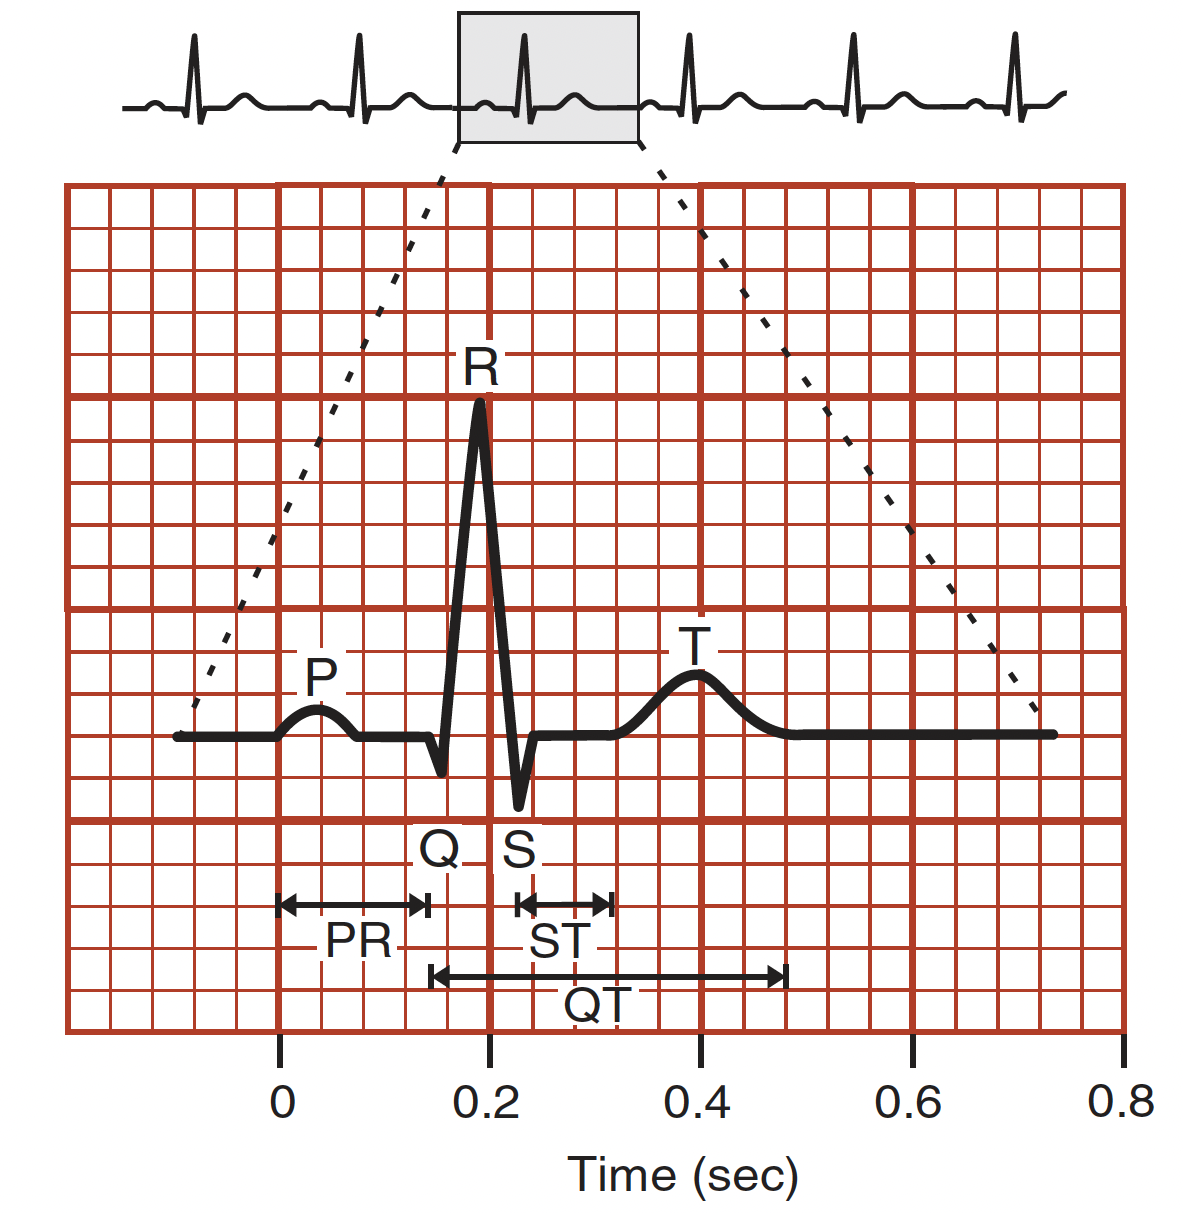
\includegraphics[width=0.5\linewidth]{images/ecg.png}
\caption{Components of the ECG trace. (\cite{alma991000225790601591})}
\label{fig:ecg-huszar}
\end{figure}

\subsection{R-peak}\label{sec:rpeaks}

The R-peak is the tallest and most prominent wave in the QRS complex of an ECG signal, the peak of the R-wave. It represents the depolarization of the left and right ventricles, which are the main pumping chambers of the heart. The ability to accurately detect R-peaks is crucial for several reasons:

\begin{itemize}
    \item Heart Rate Calculation: The time interval between consecutive R-peaks, known as the RR interval, is used to calculate the heart rate. By detecting R-peaks, we can determine the heart rate and monitor any changes or irregularities.
    \item Cardiac Rhythm Analysis: R-peak detection helps in identifying the regularity and pattern of the heart's rhythm. By analyzing the sequence of R-peaks, we can detect various arrhythmias, such as premature ventricular contractions (PVCs), atrial fibrillation, and heart blocks.
    \item Signal Quality Assessment: The consistency and clarity of R-peaks can provide insights into the overall quality of the ECG signal. If R-peaks are difficult to detect or have variable amplitudes, it may indicate the presence of noise, artifacts, or poor electrode contact.
    \item Temporal Alignment: R-peaks serve as reference points for aligning and comparing different ECG leads or signals from multiple subjects. By aligning the signals based on R-peaks, we can analyze the relative timing and morphology of other ECG components.
    \item Feature Extraction: Various features can be extracted from the ECG signal using R-peaks as anchor points. These features, such as RR intervals, QRS duration, and ST segment changes, provide valuable information for diagnosing and monitoring cardiac conditions.
\end{itemize}  
Many methods have been developed for R-peak detection, such as:
\begin{itemize}
    \item Pan-Tompkins algorithm
    \item Wavelet-based methods
    \item Hilbert transform-based methods
    \item Machine learning approaches
\end{itemize}
These algorithms aim to accurately and efficiently detect R-peaks in the presence of noise, baseline wander, and other artifacts commonly found in ECG signals. Accurate R-peak detection is essential for the reliable interpretation of ECG data and the diagnosis of various cardiac conditions.

\subsection{12-Lead ECG}\label{sec:12leads}

\noindent An ECG can contain 12 ECG traces, called 12-lead ECG. Simply said, a 12-lead ECG provides a comprehensive view of the heart's electrical activity from different angles. It consists of 12 different leads, each representing a specific view of the heart. The leads are divided into two main groups: limb leads and precordial leads. \newline

\noindent The so called  \textbf{Einthoven's Triangle} (can be seen in Figure \ref{fig:limp}) is a theoretical formation of the limb leads (I, II, III), forming an equilateral triangle with the heart at the center. This relationship helps in understanding the orientation and magnitude of the heart's electrical activity. The voltages in these leads relate to each other in the following way:

\begin{equation}
    \text{Lead I} + \text{Lead III} = \text{Lead II}.
\end{equation}

\noindent The voltages in augmented limb leads are calculated by amplifying the electrical difference between one limb electrode and a central point formed by the other limb electrodes. These relationships are based on the principle that the sum of the voltages from all three limb leads should be zero when the heart's electrical axis is normal. Let's outline the leads in the limb leads group: \newline

\noindent \textbf{Limb Leads:} The electrodes for these signals are one on each arm and one on the left leg.
\begin{itemize}
    \item \textbf{Bipolar Limb Leads} (Figure \ref{fig:limp}):
    \begin{itemize}
        \item \textbf{Lead I:} Measures the voltage difference between the left arm (LA) and right arm (RA).
        \begin{equation}
            \text{Lead I} = \text{LA} - \text{RA}
        \end{equation}
        \item \textbf{Lead II:} Measures the voltage difference between the left leg (LL) and the right arm.
        \begin{equation}
            \text{Lead II} = \text{LL} - \text{RA}
        \end{equation}
        \item \textbf{Lead III:} Measures the voltage difference between the left leg and the left arm.
        \begin{equation}
            \text{Lead III} = \text{LL} - \text{LA}
        \end{equation}
    \end{itemize}
    \item \textbf{Augmented Unipolar Limb Leads} (Figure \ref{fig:augmented}):
    \begin{itemize}
        \item \textbf{aVR:} Measures the electrical difference from the right arm to a central point between the left arm and left leg.
        \begin{equation}
            \text{aVR} = \text{RA} - \frac{1}{2}(\text{LA} + \text{LL})
        \end{equation}
        \item \textbf{aVL:} Measures the electrical difference from the left arm to a central point between the right arm and left leg.
        \begin{equation}
            \text{aVL} = \text{LA} - \frac{1}{2}(\text{RA} + \text{LL})
        \end{equation}
        \item \textbf{aVF:} Measures the electrical difference from the left leg to a central point between the right arm and left arm.
        \begin{equation}
            \text{aVF} = \text{LL} - \frac{1}{2}(\text{RA} + \text{LA})
        \end{equation}
    \end{itemize}
\end{itemize}

\begin{figure}[h]
\centering
\begin{minipage}{0.4\linewidth}
    \centering
    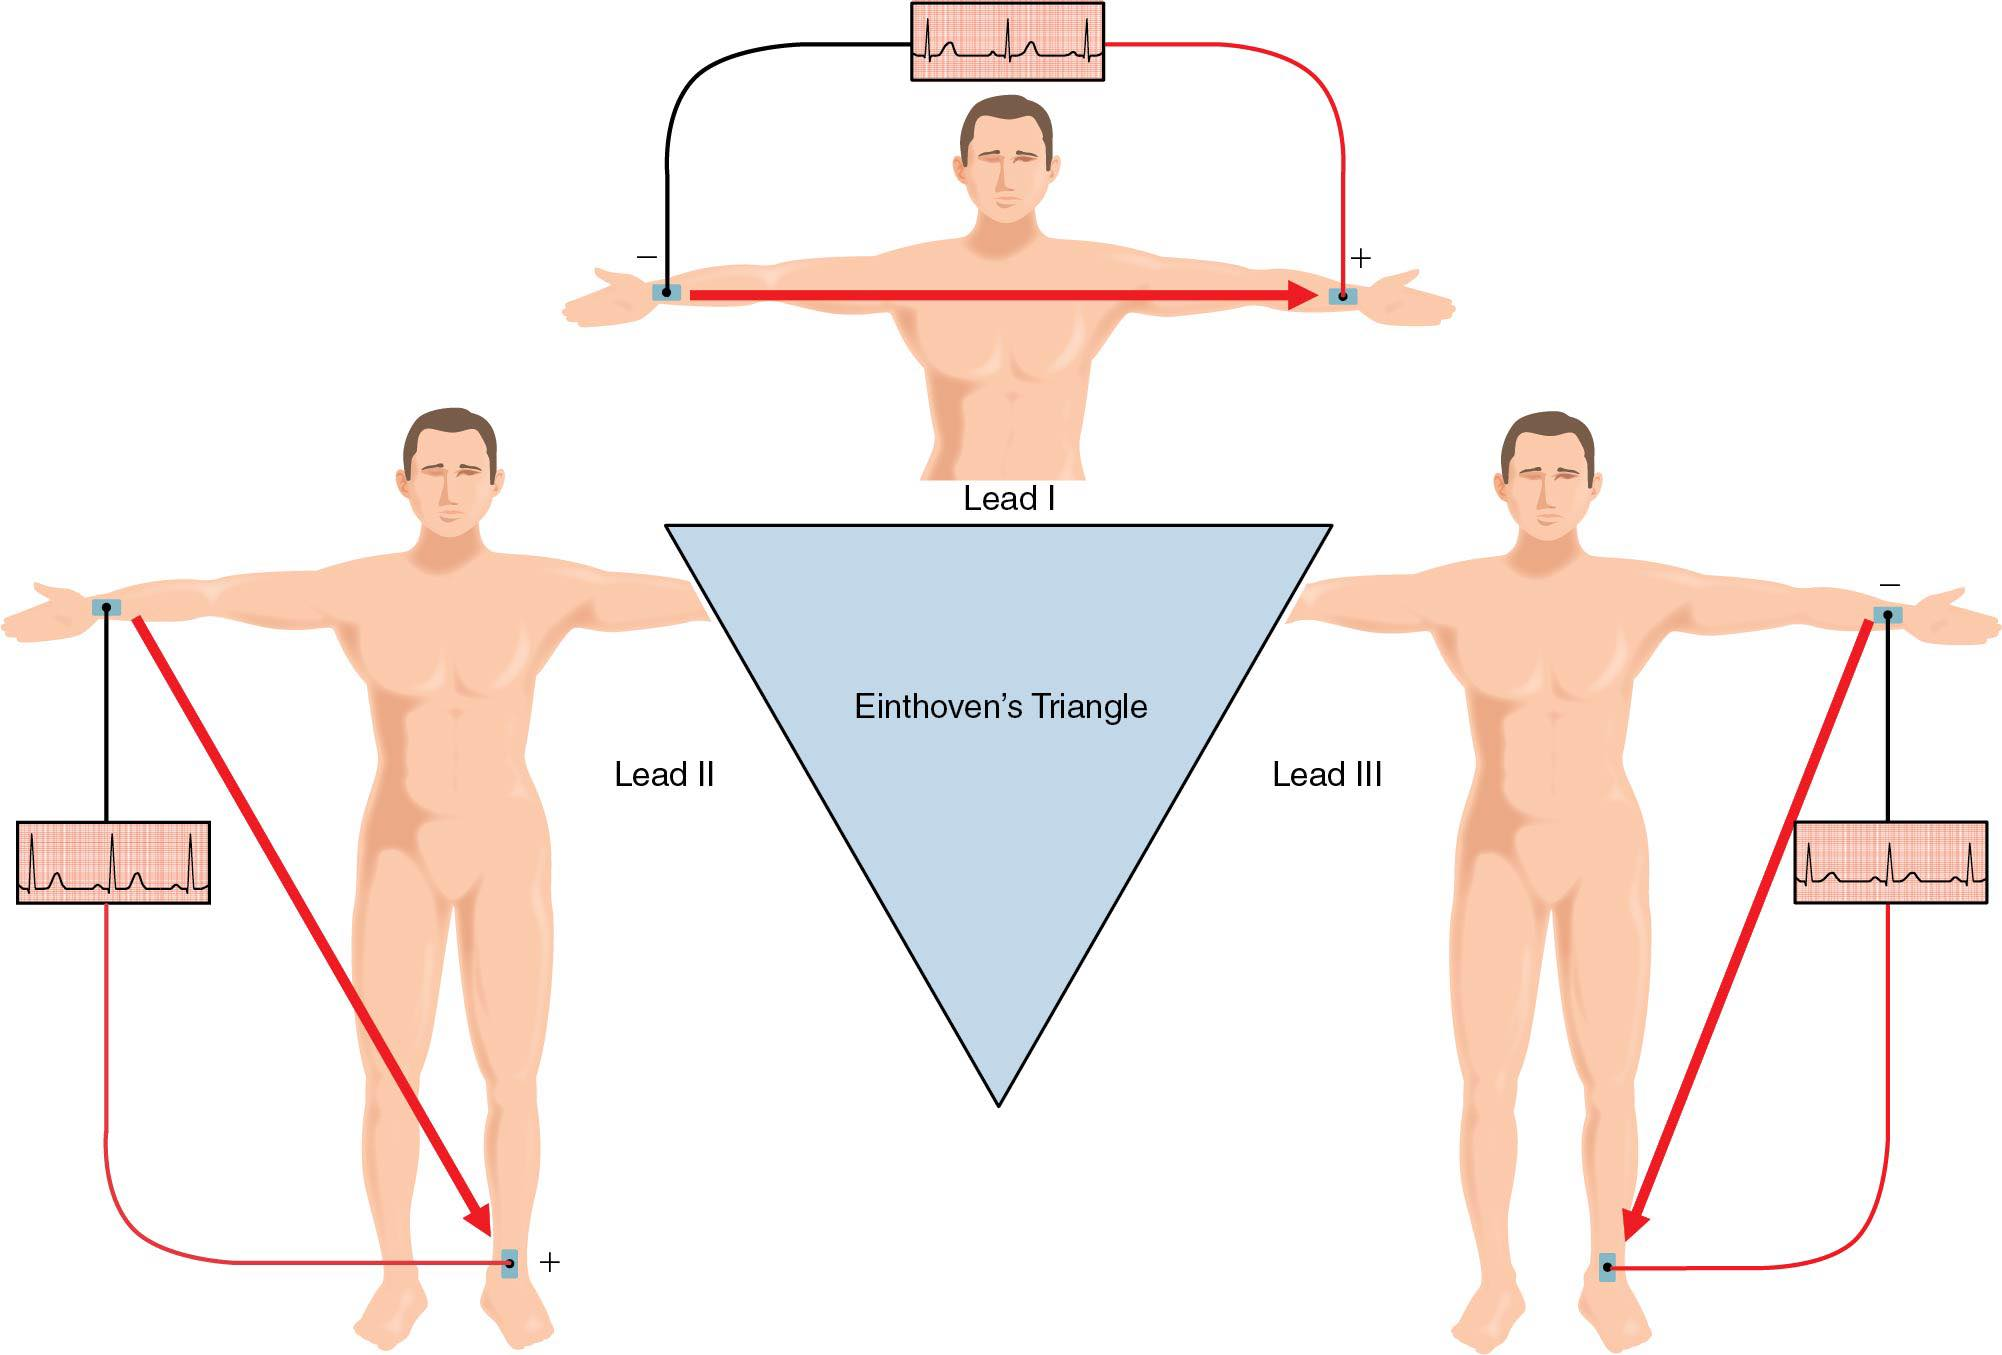
\includegraphics[width=\linewidth]{images/limp-leads-tr.jpg}
    \caption{Bipolar limb leads. (\cite{huszar})}
    \label{fig:limp}
\end{minipage}%
\hspace{0.05\linewidth}
\begin{minipage}{0.35\linewidth}
    \centering
    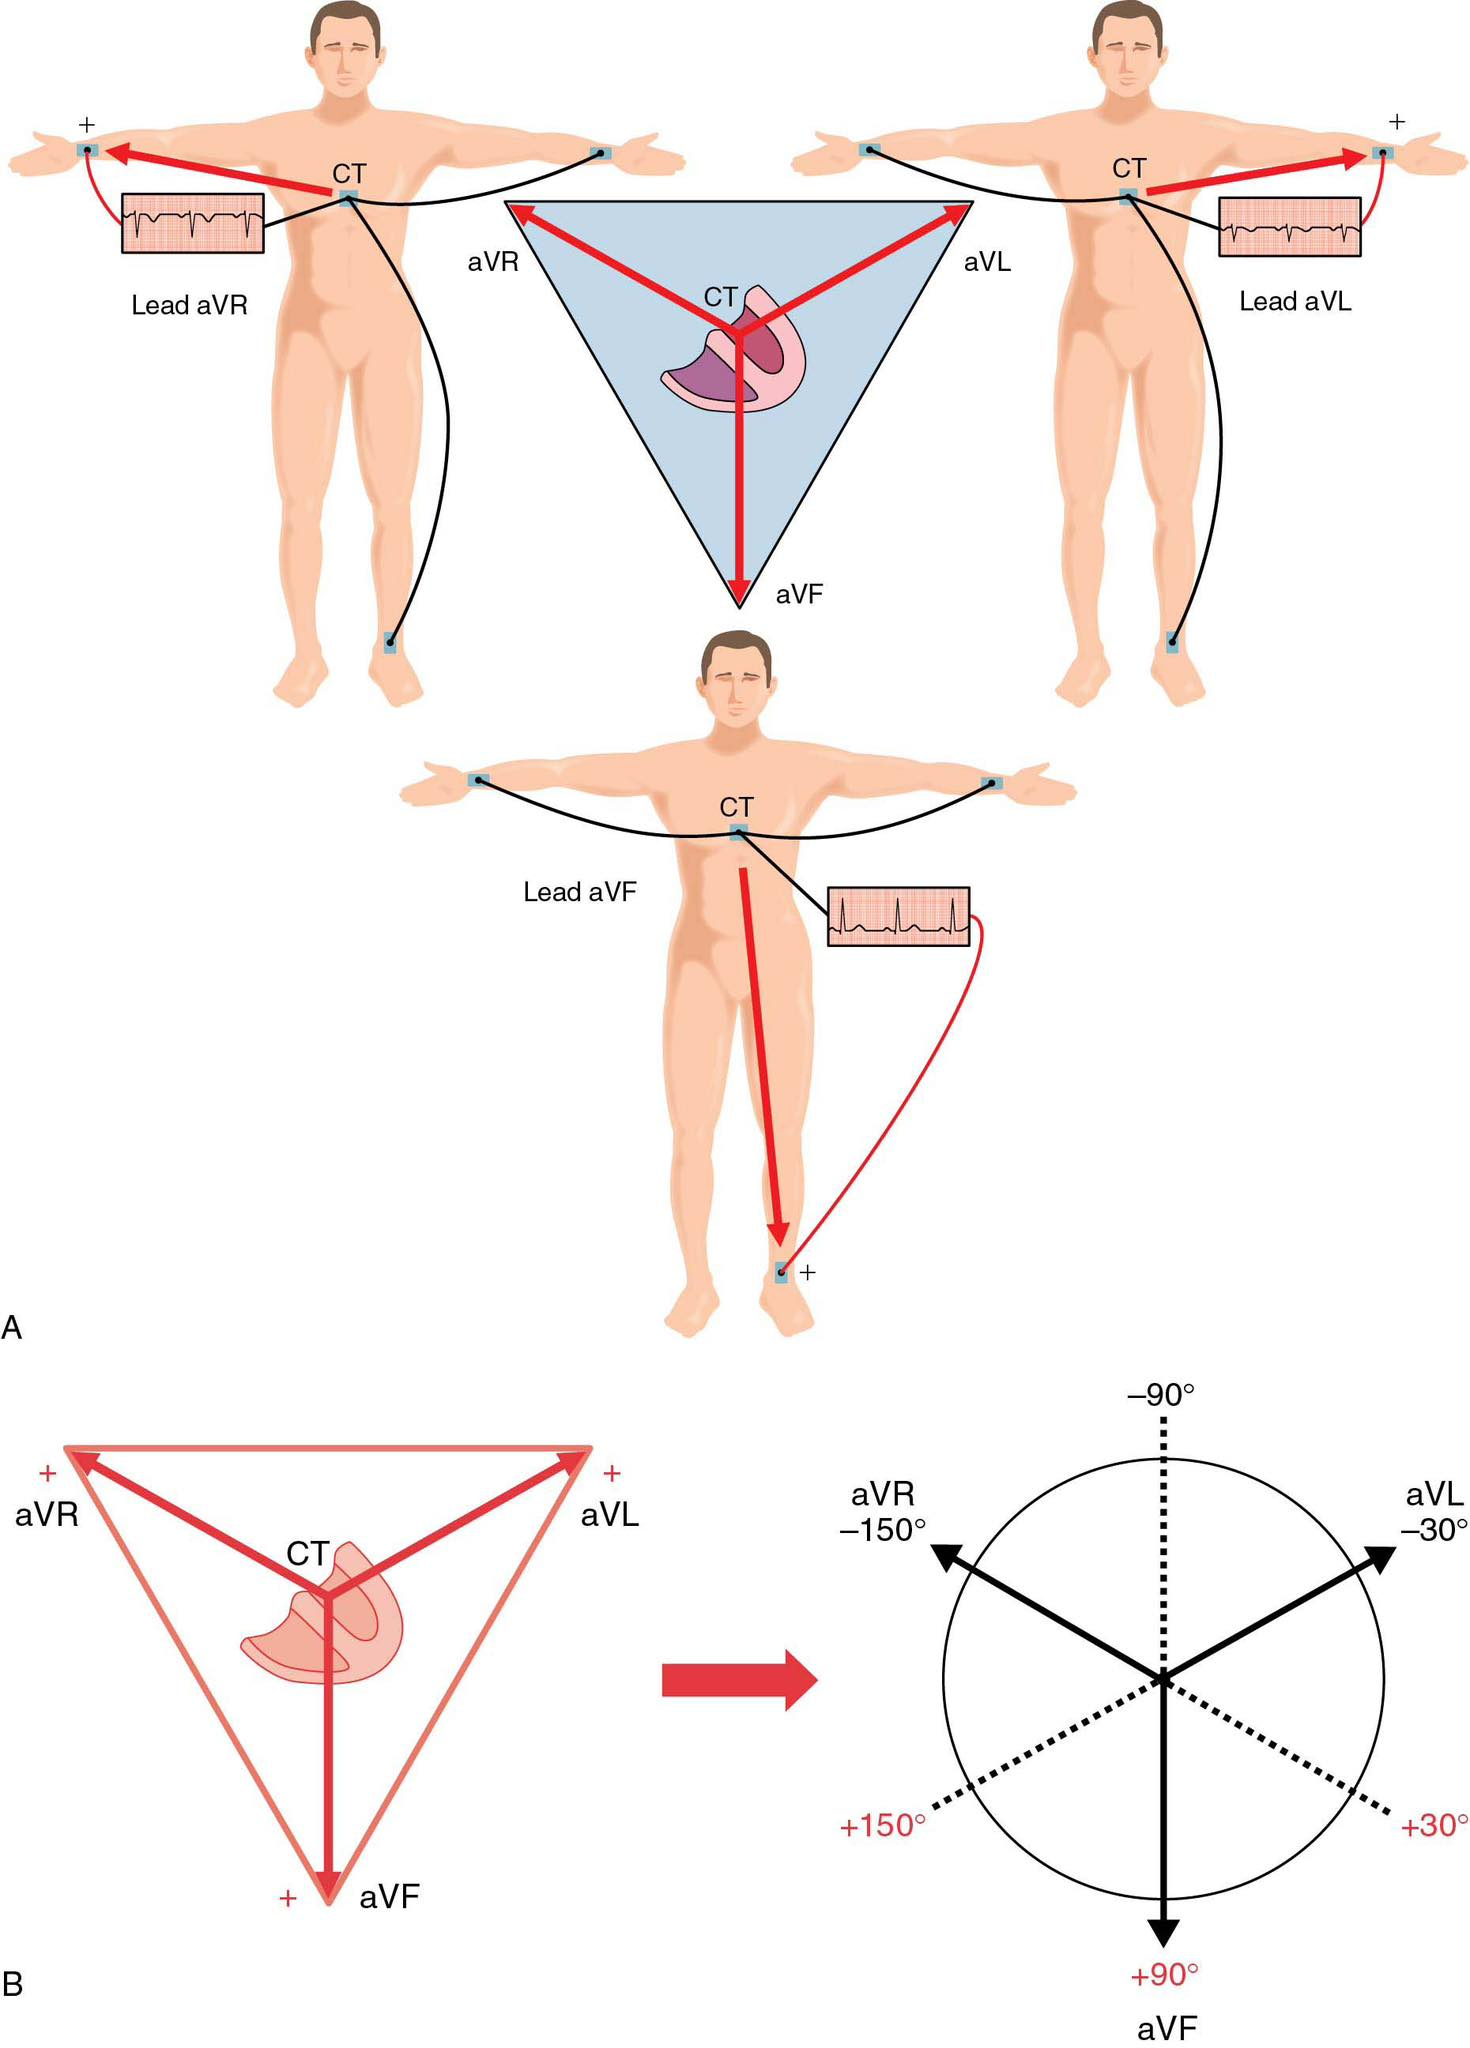
\includegraphics[width=\linewidth]{images/augmented.jpg}
    \caption{Augmented unipolar limb leads. (\cite{huszar})}
    \label{fig:augmented}
\end{minipage}
\end{figure}

\noindent The precordial leads are positioned in the horizontal plane, at right angles to the other six leads. These leads consist of six electrodes (V1 through V6) that serve as positive poles for their respective precordial leads. The negative pole for these leads is provided by Wilson's central terminal. \newline

\noindent \textbf{Precordial Unipolar Leads} (Figure \ref{fig:vs}):
\begin{itemize}
    \item \textbf{V1 to V6:} These leads provide views of the horizontal plane of the heart, from right to left.
\end{itemize}

\begin{figure}[h]
\centering
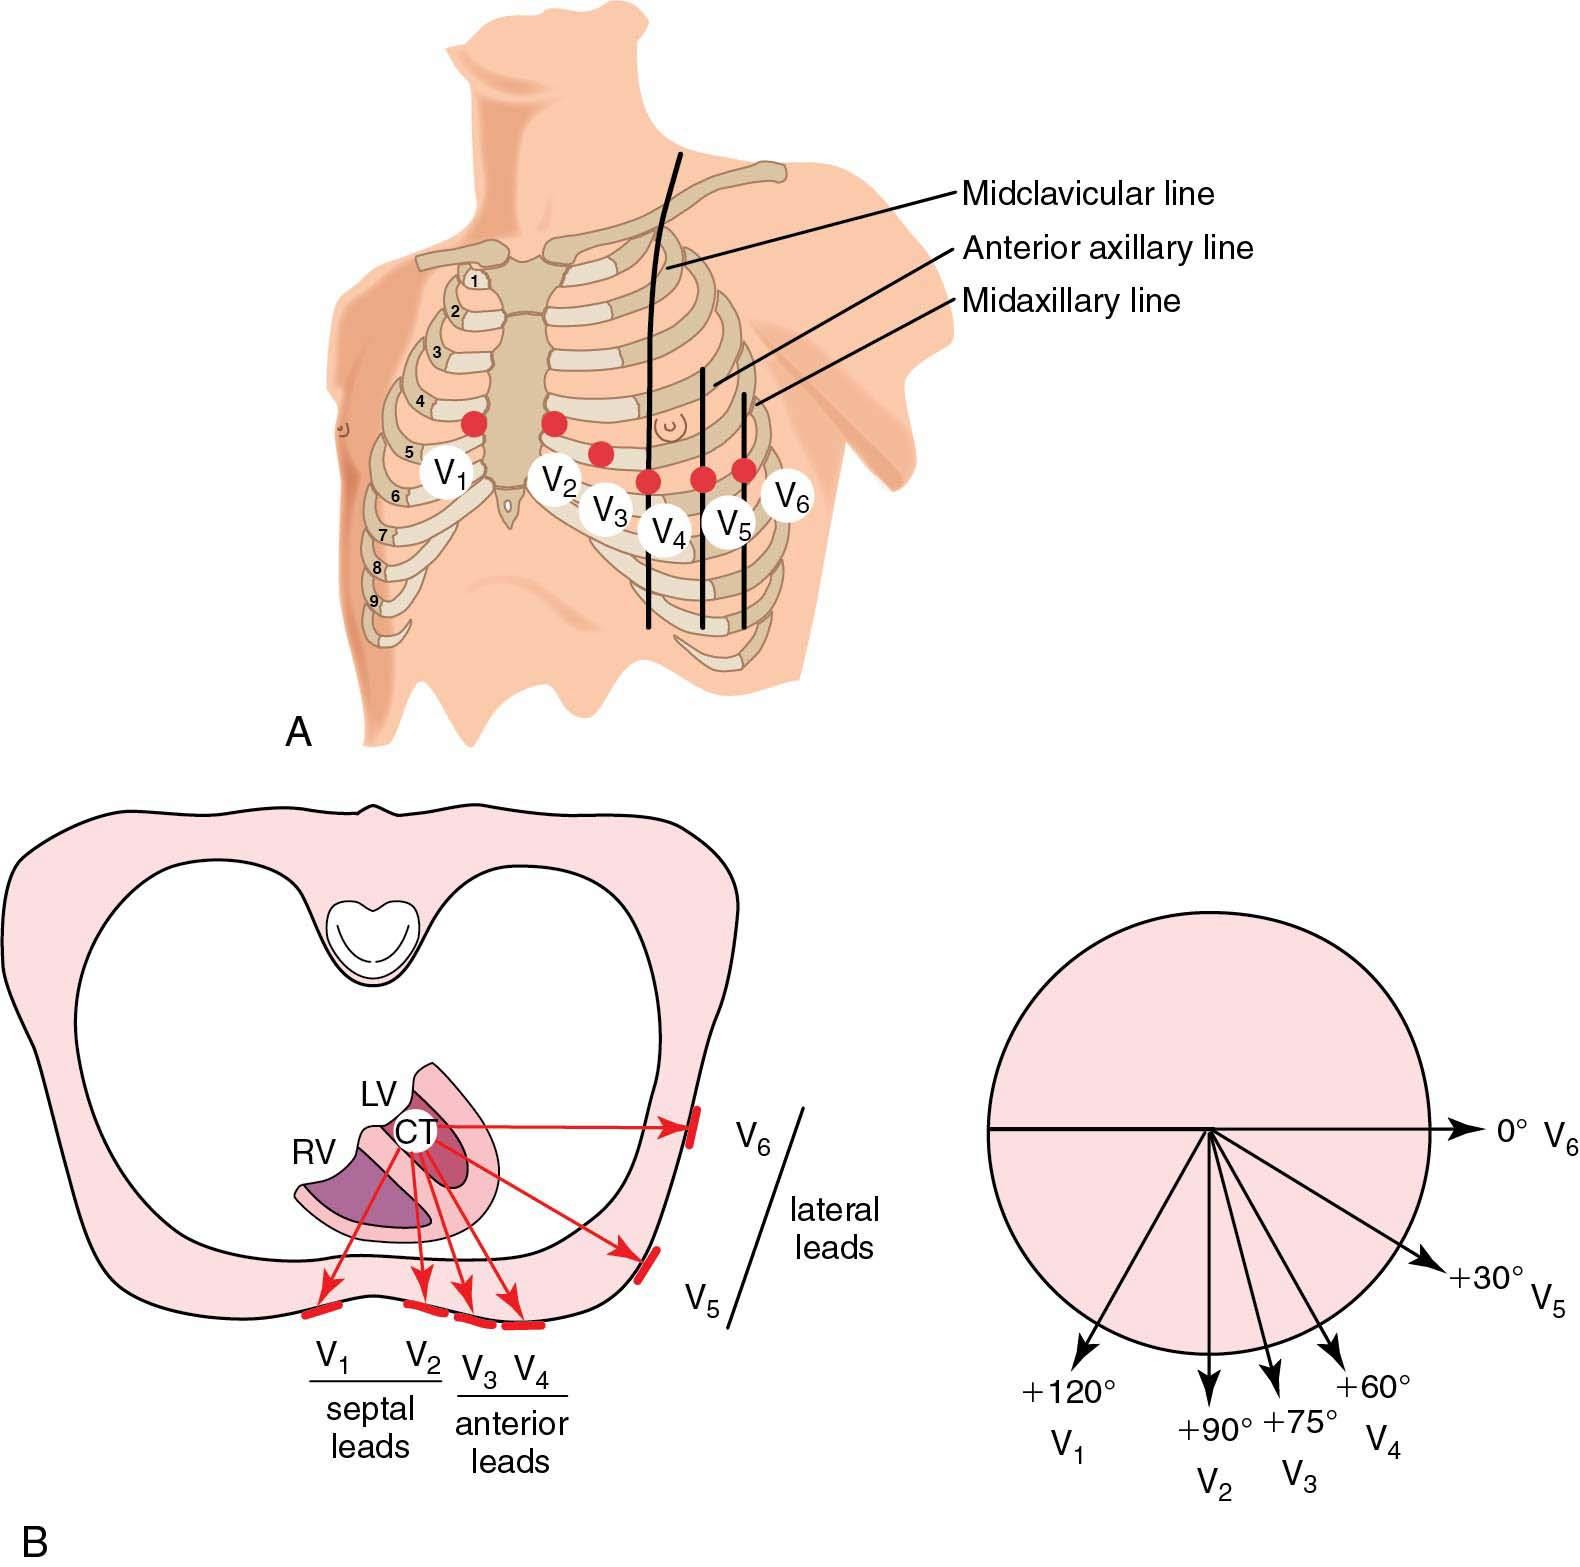
\includegraphics[width=0.3\linewidth]{images/vs.jpg}
\caption{Precordial unipolar leads. (\cite{huszar})}
\label{fig:vs}
\end{figure}

% forcing a page break
\clearpage

\chapter{Experiments and Results} \label{ch:3}

For the experiments we are going to use the already available dataset "A Large Scale 12-lead Electrocardiogram Database for Arrhythmia Study" (\cite{cite1}, \cite{cite2}, \cite{cite3}). This is a comprehensive database of high-quality 12-lead ECG signals collected from $45 152$ patients. Each signal is with length of $10$ seconds corresponding to $5 000$ data points. The dataset is designed to support arrhythmia research, containing labeled data for various cardiac conditions such as atrial fibrillation, premature ventricular contractions, and bundle branch blocks. This large dataset has high-quality labels from professional experts, diverse arrhythmia types, and additional cardiovascular conditions, making it suitable for performing our tests on it. Code to reproduce our experiments is available in an online repository.\footnote{See: https://github.com/JoeJoe1313/rPSMF} \newline

\section{Missing Data Imputation}\label{sec:exp1}

In this section, we evaluate PSMF and rPSMF on the task of imputing missing values in 12-lead ECG time-series data. 

\subsection{Data}

The 12-lead ECG signal is chosen to be one representing a normal heart rhythm (sinus rhythm). As already mentioned each of the $m = 12$ leads contains $n = 5000$ data points. One heart beat (PQRST complex) is of approximate length of $300$ data points. That's why, to assess the imputation accuracy, we choose to randomly remove segments of length $300$ from the signal, and construct datasets with $20\%$, $30\%$, and $40\%$ missing data. We compare the results for each dataset against two other baseline sequential methods used in \cite{akyildiz2021probabilistic}. The first, which we call MLE-SMF, is a maximum likelihood estimation (MLE) method for online probabilistic matrix factorization where the state transition matrix $C$ remains constant over time. This builds on prior work by \cite{YILDIRIM2012494}, \cite{6288274}, and \cite{6638240}. The second approach adapts the temporal matrix factorization (TMF) optimization technique proposed by \cite{NIPS2016_85422afb}. \newline

\subsection{Models}

\noindent For PSMF and rPSMF we choose a random walk subspace model $f_{\theta}(x) = x$, and for the imputation we use the final estimates of $C$ and $X$. We test the four sequential models by setting the rank first to $r = 3$, and then to $r = 10$. As in \cite{akyildiz2021probabilistic}, for TMF we set the weight matrix to identity, for PSMF and MLE- SMF we set $R_k := R = \rho \otimes I_m$, where $\rho = 10$, $P_0 = I_r$, $Q_k := Q = q \otimes I_r$, and $q = 0.1$. For rPSMF we use $R_0 = R$ and $Q_0 = Q$ and choose $\lambda_0 = 1.8$, and for both PSMF and rPSMF we set $V_0 = v_0 \otimes I_r$ with $v_0 = 2$. We evaluate the performance of the four methods PSMF, rPSMF, MLE-SMF, and TMF by running each of them for two epochs. To ensure the robustness and reliability of our findings, we conduct the experiments $100$ times, each time using different initialization and randomly generated patterns of missing data. \newline

\subsection{Results}

\noindent Table \ref{tab:rmse3} presents the results for rank $r = 3$ across scenarios with $20\%$, $30\%$, and $40\%$ missing data. The findings show that PSMF and rPSMF achieve lower imputation Root Mean Square Errors (RMSEs) than MLE-SMF and TMF, with rPSMF slightly outperforming PSMF. For rank $r = 10$, as shown in Table \ref{tab:rmse10}, PSMF emerges as the top performer across all test cases. While MLE-SMF and TMF results remain relatively consistent with their rank $r = 3$ performance, rPSMF shows a significant decline in performance, severely worsening as the percentage of missing data increases. PSMF's performance is also worse than for $r = 3$ but it is not that much affected as rPSMF. This observation contradicts our initial hypothesis that higher rank might lead to lower imputation RMSE, and is caused by overfitting. \newline

\begin{table}[H]
\centering
\text{$r = 3$} \\[0.5ex]
\begin{tabular}{@{}lccc|ccccc@{}}
\toprule
 & \multicolumn{3}{c}{Imputation RMSE} & \multicolumn{3}{c}{Runtime (s)} \\
 & 20\% & 30\% & 40\% & 20\% & 30\% & 40\% \\
\midrule
PSMF & $\underset{{\scriptscriptstyle \;\;(32.19)}}{104.46}$ & $\underset{{\scriptscriptstyle \;\;(31.61)}}{115.99}$ & $\underset{{\scriptscriptstyle \;\;\;(31.77)}}{138.18}$ & 0.58 & 0.59 & 0.58 \\
rPSMF & $\underset{{\scriptscriptstyle \;\;(26.56)}}{\textbf{98.51}}$ & $\underset{{\scriptscriptstyle \;\;(29.08)}}{\textbf{109.04}}$ & $\underset{{\scriptscriptstyle \;\;(29.58)}}{\textbf{124.91}}$ & 0.65 & 0.64 & 0.64 \\
MLE-SMF & $\underset{{\scriptscriptstyle \;\;\;(34.07)}}{271.04}$ & $\underset{{\scriptscriptstyle \;\;\;(33.46)}}{263.65}$ & $\underset{{\scriptscriptstyle \;\;\;(28.69)}}{244.21}$ & 0.50 & 0.51 & 0.50 \\
TMF & $\underset{{\scriptscriptstyle \;\;\;(16.18)}}{202.76}$ & $\underset{{\scriptscriptstyle \;\;\;(15.97)}}{202.90}$ & $\underset{{\scriptscriptstyle \;\;\;(19.24)}}{208.98}$ & 0.28 & 0.28 & 0.27 \\
\bottomrule
\end{tabular}
\caption{Imputation error and runtime using 20\%, 30\% and 40\% missing values, rank 3, averaged over 100 random repetitions.}
\label{tab:rmse3}
\end{table}

\begin{table}[H]
\centering
\text{$r = 10$} \\[0.5ex]
\begin{tabular}{@{}lccc|ccccc@{}}
\toprule
 & \multicolumn{3}{c}{Imputation RMSE} & \multicolumn{3}{c}{Runtime (s)} \\
 & 20\% & 30\% & 40\% & 20\% & 30\% & 40\% \\
\midrule
PSMF & $\underset{{\scriptscriptstyle \;\;(38.89)}}{\textbf{122.79}}$ & $\underset{{\scriptscriptstyle \;\;(45.69)}}{\textbf{154.79}}$ & $\underset{{\scriptscriptstyle \;\;\;(52.85)}}{\textbf{186.31}}$ & 0.92 & 1.07 & 1.07 \\
rPSMF & $\underset{{\scriptscriptstyle \;\;(71.96)}}{192.19}$ & $\underset{{\scriptscriptstyle \;\;(92.27)}}{253.77}$ & $\underset{{\scriptscriptstyle \;\;(132.56)}}{377.75}$ & 1.10 & 1.08 & 1.07\\
MLE-SMF & $\underset{{\scriptscriptstyle \;\;\;(21.63)}}{268.57}$ & $\underset{{\scriptscriptstyle \;\;\;(30.37)}}{267.81}$ & $\underset{{\scriptscriptstyle \;\;\;(33.82)}}{270.77}$ & 0.82 & 0.90 & 0.90 \\
TMF & $\underset{{\scriptscriptstyle \;\;\;(20.04)}}{205.67}$ & $\underset{{\scriptscriptstyle \;\;\;(17.31)}}{199.81}$ & $\underset{{\scriptscriptstyle \;\;\;(20.25)}}{193.28}$ & 0.42 & 0.47 & 0.44 \\
\bottomrule
\end{tabular}
\caption{Imputation error and runtime using 20\%, 30\% and 40\% missing values, rank 10, averaged over 100 random repetitions.}
\label{tab:rmse10}
\end{table}

\noindent  We can evaluate the effectiveness of our uncertainty quantification by calculating the percentage of missing values that fall within a two-standard-deviation ($2\sigma$) interval of the approximate posterior distribution. The results, presented in Table \ref{tab:coverage}, show that rPSMF has the most coverage compared to PSMF and MLE-SMF (TMF does not provide a posterior distribution). While rPSMF has the highest coverage we can notice that it lowers when the rank is higher. For PSMF the coverage improves as the rank is higher. MLE-SMF has the same coverage for both ranks.

\begin{table}[H]
    \centering
    \begin{minipage}{0.45\textwidth}
        \centering
        \text{$r = 3$} \\[0.5ex]
        \begin{threeparttable}
            \begin{tabular}{lccc}
                \hline
                Missing \%: & 20\% & 30\% & 40\% \\
                \hline
                PSMF & 0.14 & 0.12 & 0.10 \\
                rPSMF & \textbf{0.80} & \textbf{0.75} & \textbf{0.66} \\
                MLE-SMF & 0.07 & 0.06 & 0.06 \\
                \hline
            \end{tabular}
        \end{threeparttable}
    \end{minipage}%
    \hspace{0.1\textwidth}%
    \begin{minipage}{0.45\textwidth}
        \centering
        \text{$r = 10$} \\[0.5ex]
        \begin{threeparttable}
            \begin{tabular}{lccc}
                \hline
                Missing \%: & 20\% & 30\% & 40\% \\
                \hline
                PSMF & 0.24 & 0.18 & 0.14 \\
                rPSMF & \textbf{0.60} & \textbf{0.50} & \textbf{0.37} \\
                MLE-SMF & 0.07 & 0.06 & 0.05 \\
                \hline
            \end{tabular}
        \end{threeparttable}
    \end{minipage}
    \caption{Average coverage proportion of the missing data by the $2\sigma$ uncertainty bars of the posterior predictive estimates, averaged over 100 repetitions. Left: results for rank 3, right: results for rank 10.}
    \label{tab:coverage}
\end{table}

\begin{figure}[h!]
\centering
\begin{minipage}{0.4\linewidth}
    \centering
    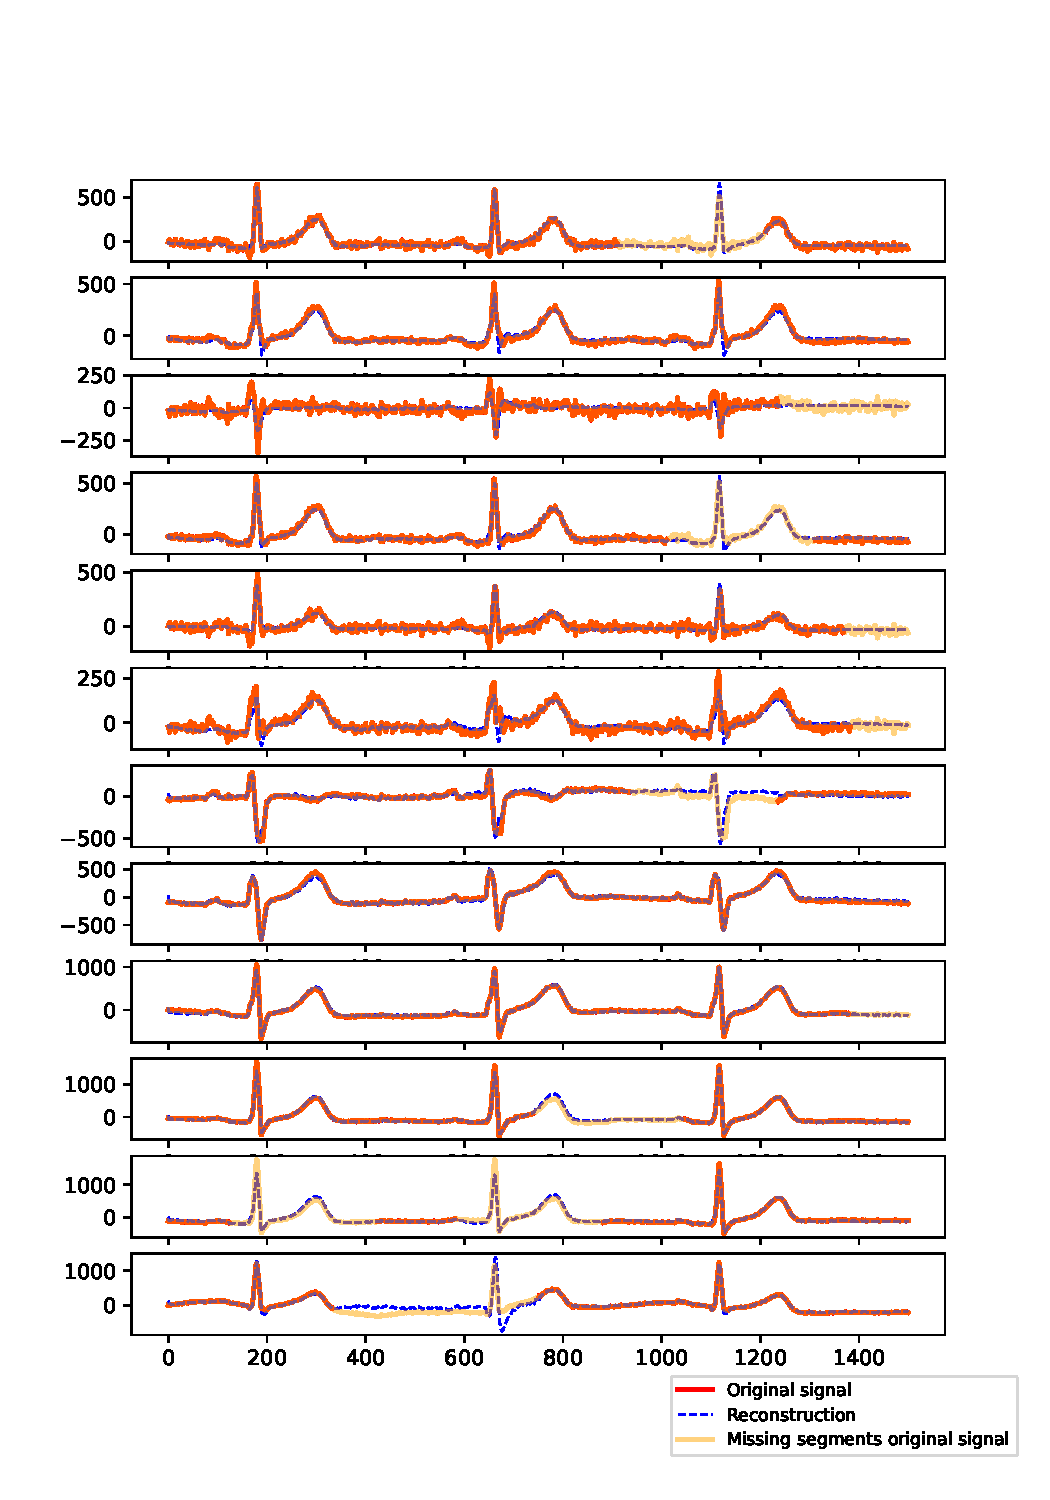
\includegraphics[width=\linewidth]{images/missing/psmf_output_20_3_half.pdf}
\end{minipage}%
\hspace{0.05\linewidth}
\begin{minipage}{0.4\linewidth}
    \centering
    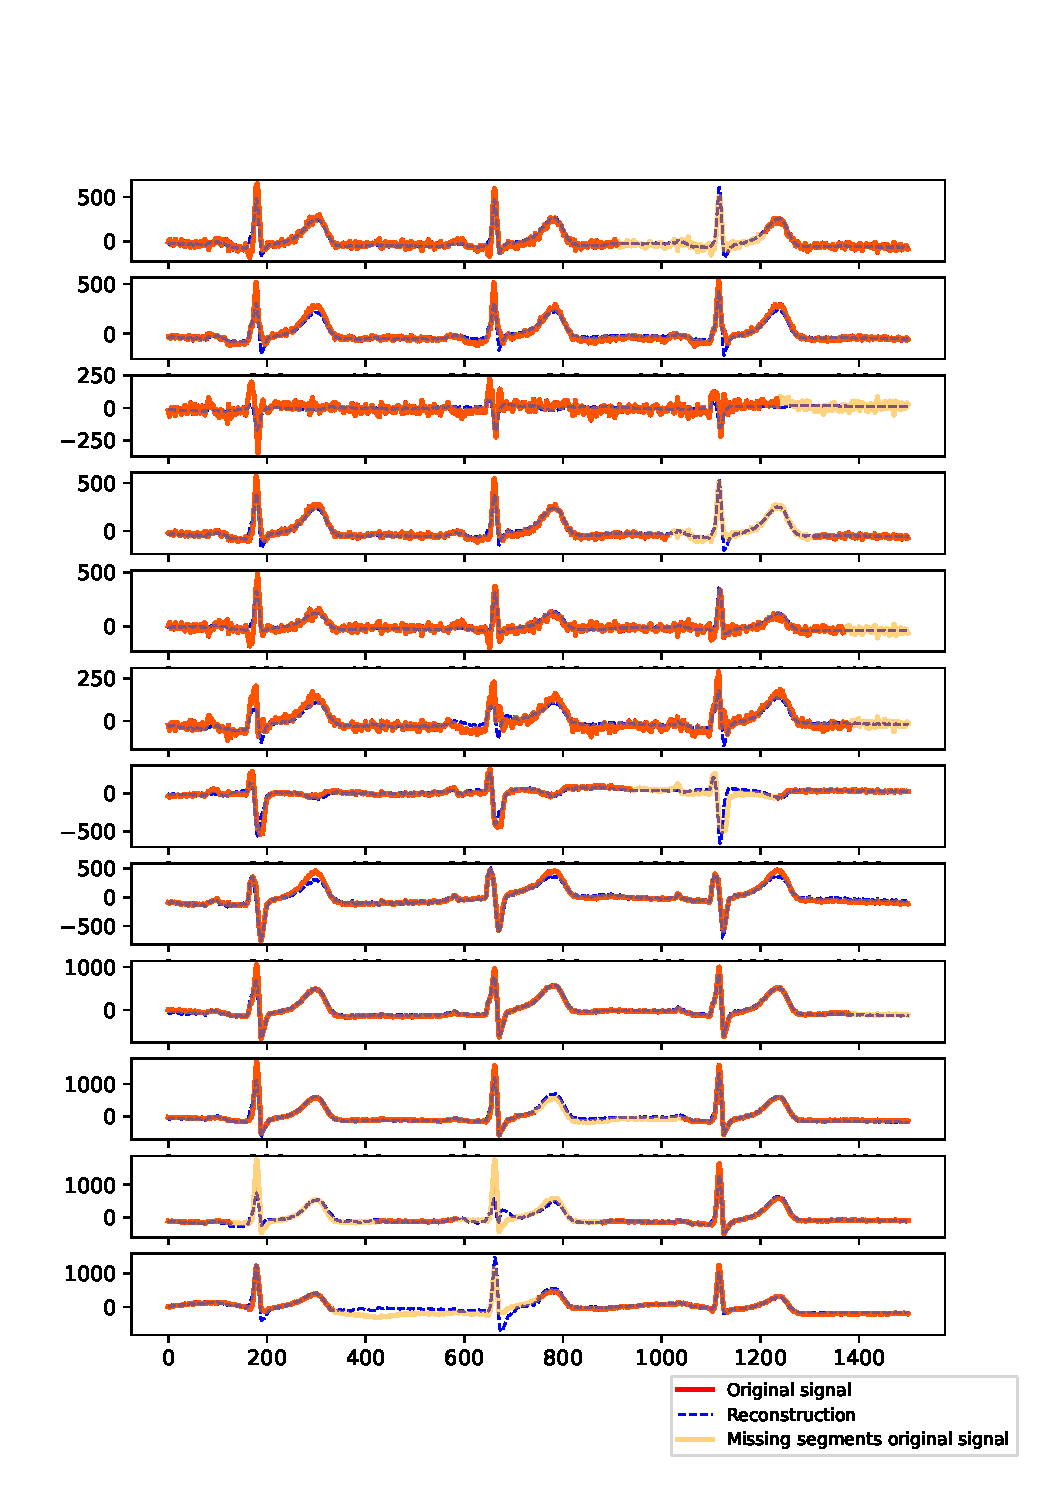
\includegraphics[width=\linewidth]{images/missing/rpsmf_output_20_3_half.pdf}
\end{minipage}
\caption{Reconstruction of the first $1500$ data points with rank 3 of 20\% missing data. Left: PSMF; Right: rPSMF.}
\label{fig:mrec3}
\end{figure}

\begin{figure}[h!]
\centering
\begin{minipage}{0.4\linewidth}
    \centering
    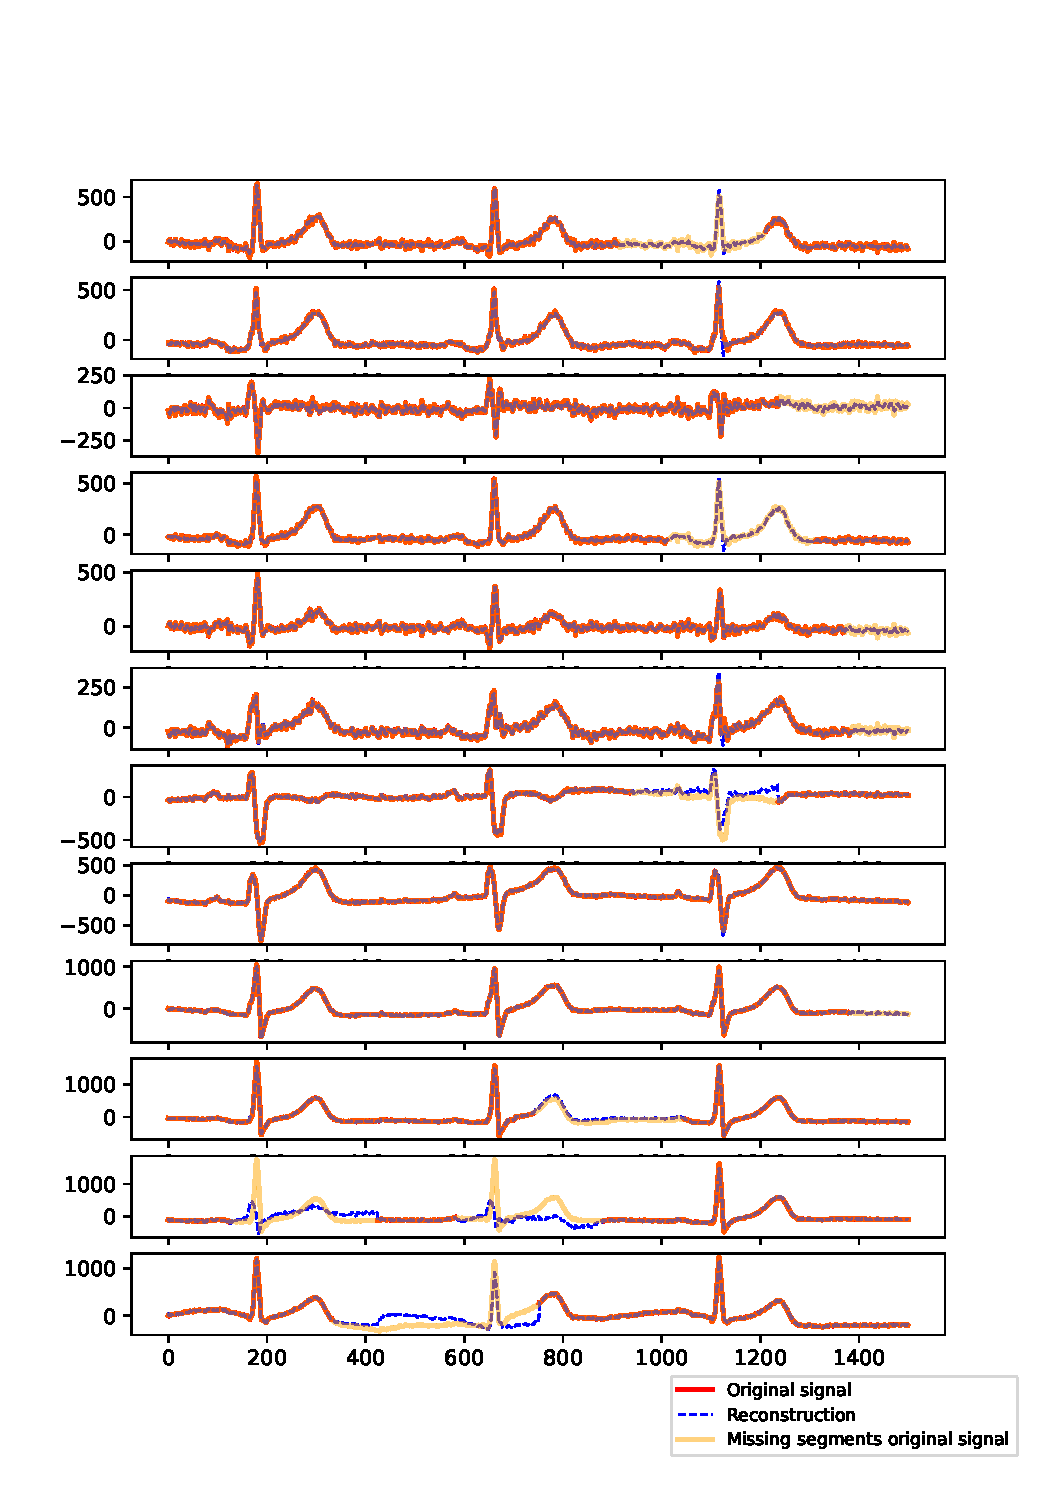
\includegraphics[width=\linewidth]{images/missing/psmf_output_20_10_half.pdf}
    \label{fig:limp}
\end{minipage}%
\hspace{0.05\linewidth}
\begin{minipage}{0.4\linewidth}
    \centering
    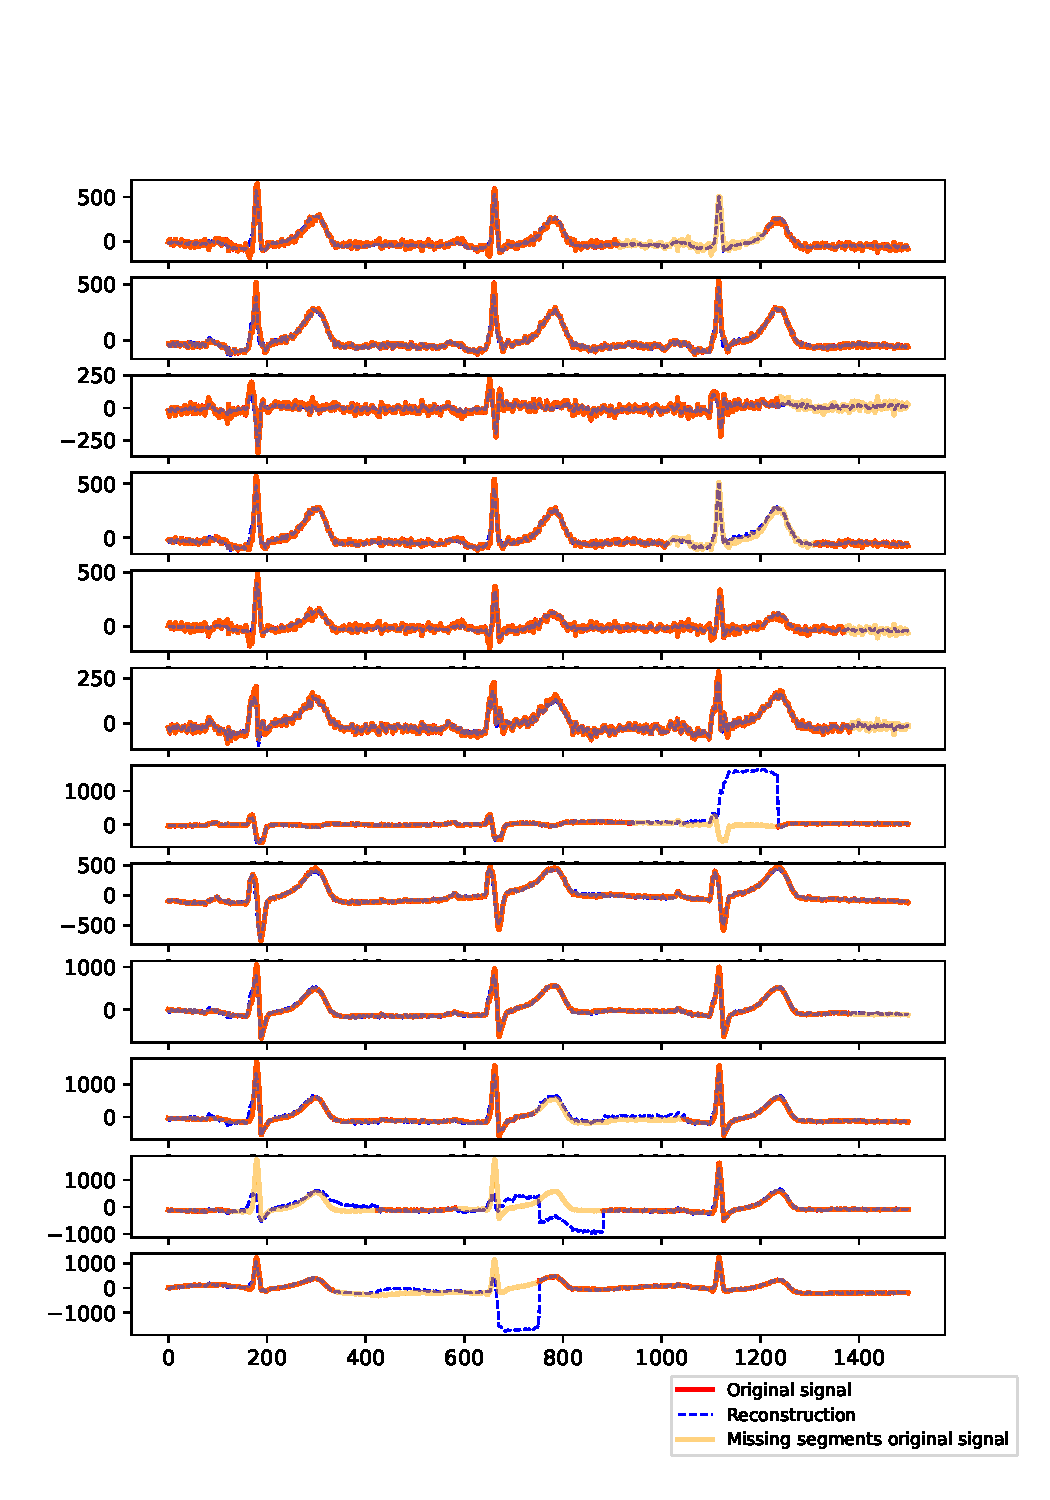
\includegraphics[width=\linewidth]{images/missing/rpsmf_output_20_10_half.pdf}
    \label{fig:augmented}
\end{minipage}
\caption{Reconstruction of the first $1500$ data points with rank 10, 20\% coverage. Left: PSMF; Right: rPSMF.}
\label{fig:mrec10}
\end{figure}

\noindent In Figure \ref{fig:mrec3} we can see reconstructions of the first $1500$ data points of the 12-lead ECG signal with rank $r = 3$ and $20\%$ missing data achieved by applying PSMF (left) and rPSMF (right). The parts in orange correspond to the segments of length $300$ we have randomly removed, the red parts are the non-missing ones from the original signal, and the reconstruction is shown with a blue dashed line. There are missing parts containing a whole heart beat, parts of the heart beat, or parts between two heart beats. We can observe that both PSMF and rPSMF manage to capture the dynamics of the signal, with PSMF visually doing a better job with the high amplitude of the R wave in missing heart beats, especially in the beginning of the signal. In Figure \ref{fig:mrec10} we can see reconstructions of the same 12-lead ECG signal but with rank $r = 10$ and $20\%$ missing data achieved by applying PSMF (left) and rPSMF (right). It is noticeable that PSMF has generally worse reconstruction than for rank $r = 3$, with some of the R wave amplitudes being too low or too high. For rPSMF in some of the leads we can see very big discrepancies between the reconstruction and the original signal. All of the visualisations for all $5000$ data points for PSMF, rPSMF, MLE-SMF, and TMF for both ranks $3$ and $10$ and the three scenarios with $20\%$, $30\%$, and $40\%$ missing data can be found in Appendix \ref{app:mdi}. \newline

\subsection{Conclusion}

\noindent In this section, we evaluated the performance of PSMF and rPSMF on the task of imputing missing values in 12-lead ECG time-series data, comparing them against MLE-SMF and TMF as baselines. Our experiments, conducted across various missing data scenarios and matrix ranks, reveal that PSMF and rPSMF generally outperform the baseline methods in terms of lower imputation RMSE, particularly at a lower rank of $r = 3$. Notably, rPSMF consistently achieved the best performance for rank $3$ across all levels of missing data, though its efficacy diminished significantly at the higher rank of $r = 10$, especially as the proportion of missing data increased. Additionally, our uncertainty quantification analysis indicated that rPSMF provided the highest coverage of the missing data within a $2\sigma$ interval, although this coverage decreased with increasing rank. Visual inspection of the reconstructions further corroborated the quantitative findings, with PSMF showing superior performance, particularly in retaining the high amplitude of the R wave. Overall, these results highlight the strengths and limitations of both PSMF and rPSMF in handling missing data in ECG signals and suggest that rank selection plays a crucial role in their effectiveness.

\section{R-peaks Detection}\label{sec:rpeaksdet}

As discussed in Section \ref{sec:rpeaks}, precise R-peak detection is crucial for accurate ECG data interpretation and cardiac condition diagnosis. Our numerous unsuccessful attempts to forecast the high-amplitude, sharp R waves with PSMF resulted in predictions with lower amplitudes and smoother peaks. This consistent forecasting challenge inspired us to explore a novel approach: leveraging this prediction discrepancy as a method for R-peak detection.

\subsection{R-peaks Detection Method}

\noindent Here, we outline the main approach steps for R-peak detection:
\begin{itemize}
    \item Apply PSMF to achieve smoother lower amplitude R wave forecast
    \item Remove the reconstruction from the original data
    \item Define a threshold as a percentile of the differences between the reconstruction and the original data
    \item Determine the points above this threshold as R-peaks
\end{itemize}

\subsection{Data}

\noindent For this experiment we are going to work with the same sinus rhythm signal as in Section \ref{sec:exp1}. For demonstrating the approach steps we are going to show only the results for the Lead II signal. \newline

\noindent To ease the computational resources needed we are going to work with a resampled version of the signal. The resampling would make the original signal (Figure \ref{fig:orig-ecg}) from containing $5000$ points to containing only $1500$ points (Figure \ref{fig:resampled-ecg}). This is achieved by first applying Fast Fourier Transform (FFT) to transform the original signal into the frequency domain, then removing coefficients from the higher frequency components, effectively performing a low-pass filter, and finally applying an Inverse Fast Fourier Transform (IFFT) to convert the modified frequency domain signal back to the time domain. For clarity, this is done by using the \texttt{resample} function from the Python library \texttt{scipy.signal}. Observing Figure \ref{fig:orig-ecg} and Figure \ref{fig:resampled-ecg} confirms that the original structure and important characteristics of the data are preserved. \newline

\begin{figure}[h]
\centering
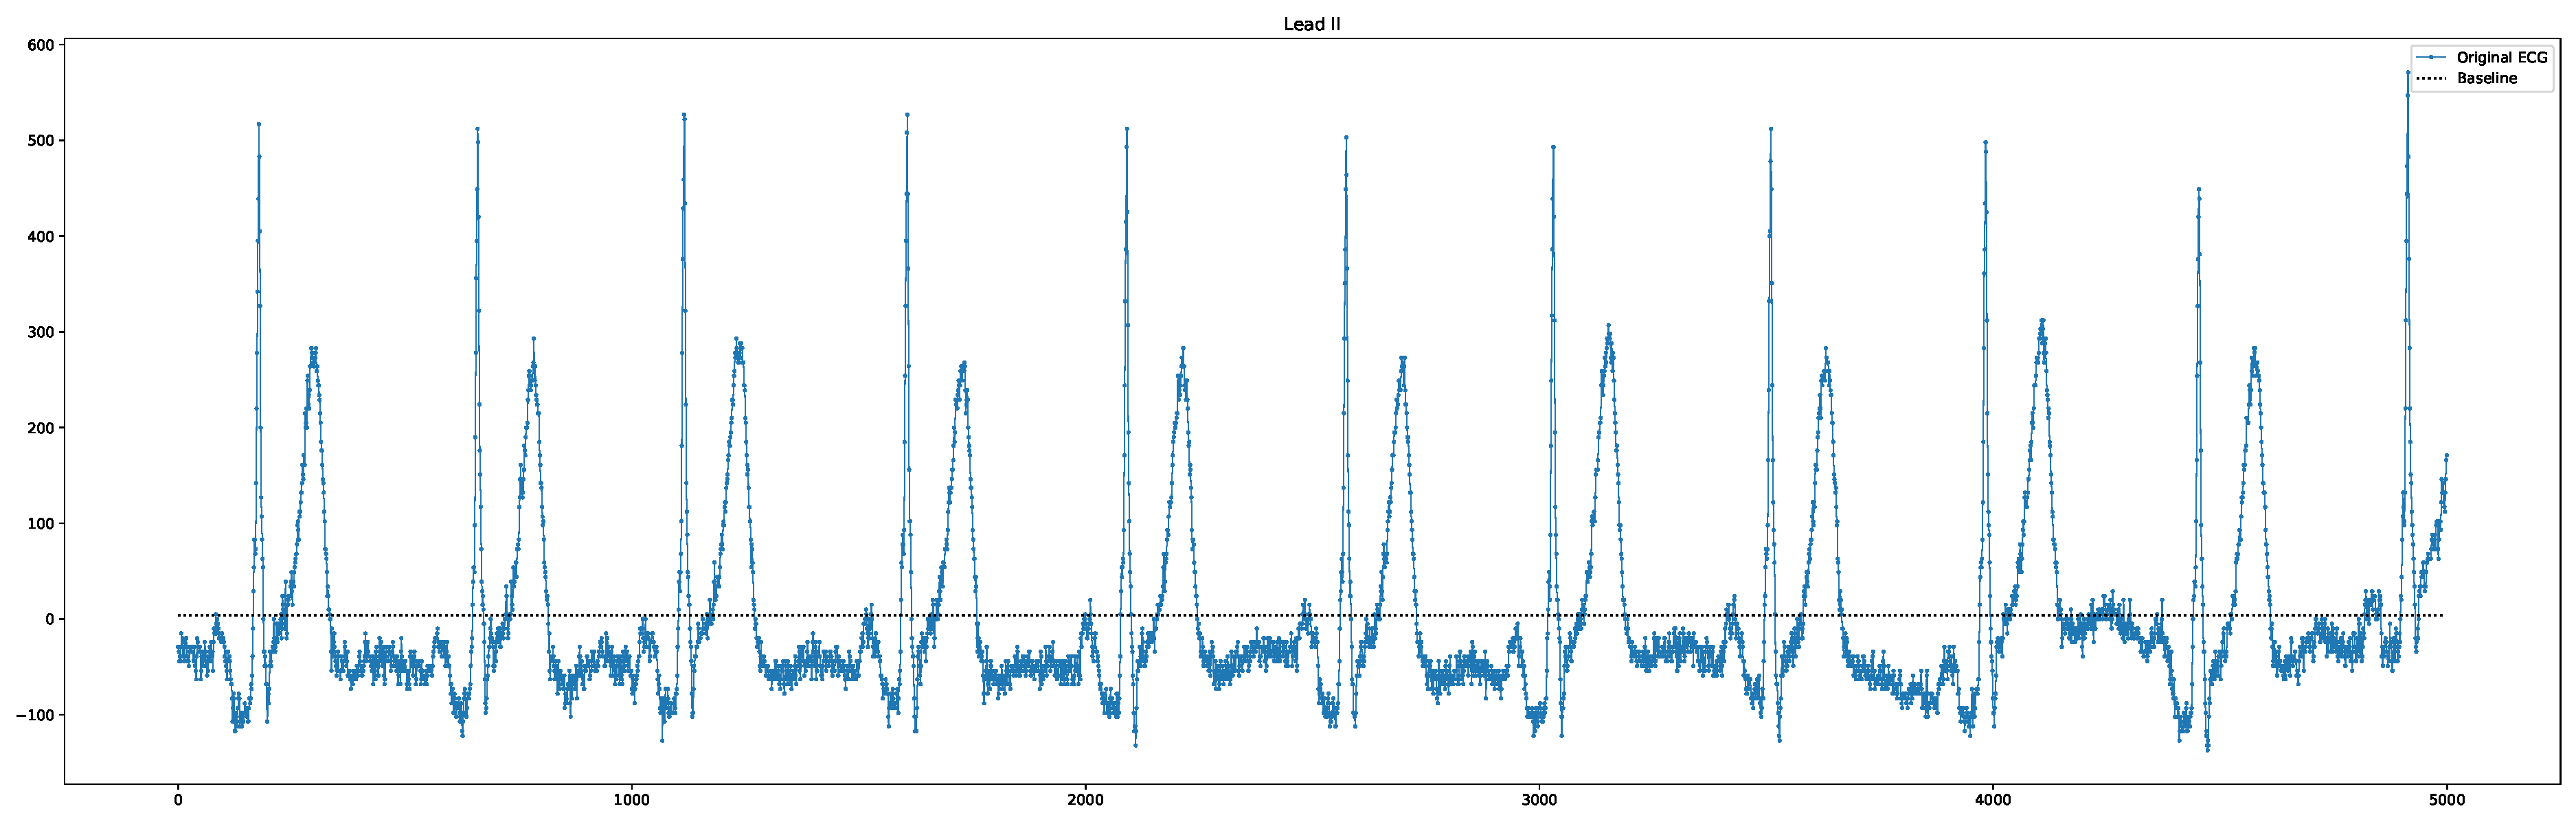
\includegraphics[width=1\linewidth]{images/r_peaks/original_ecg_m.pdf}
\caption{Original Lead II signal, 5000 points.}
\label{fig:orig-ecg}
\end{figure}

\begin{figure}[h]
\centering
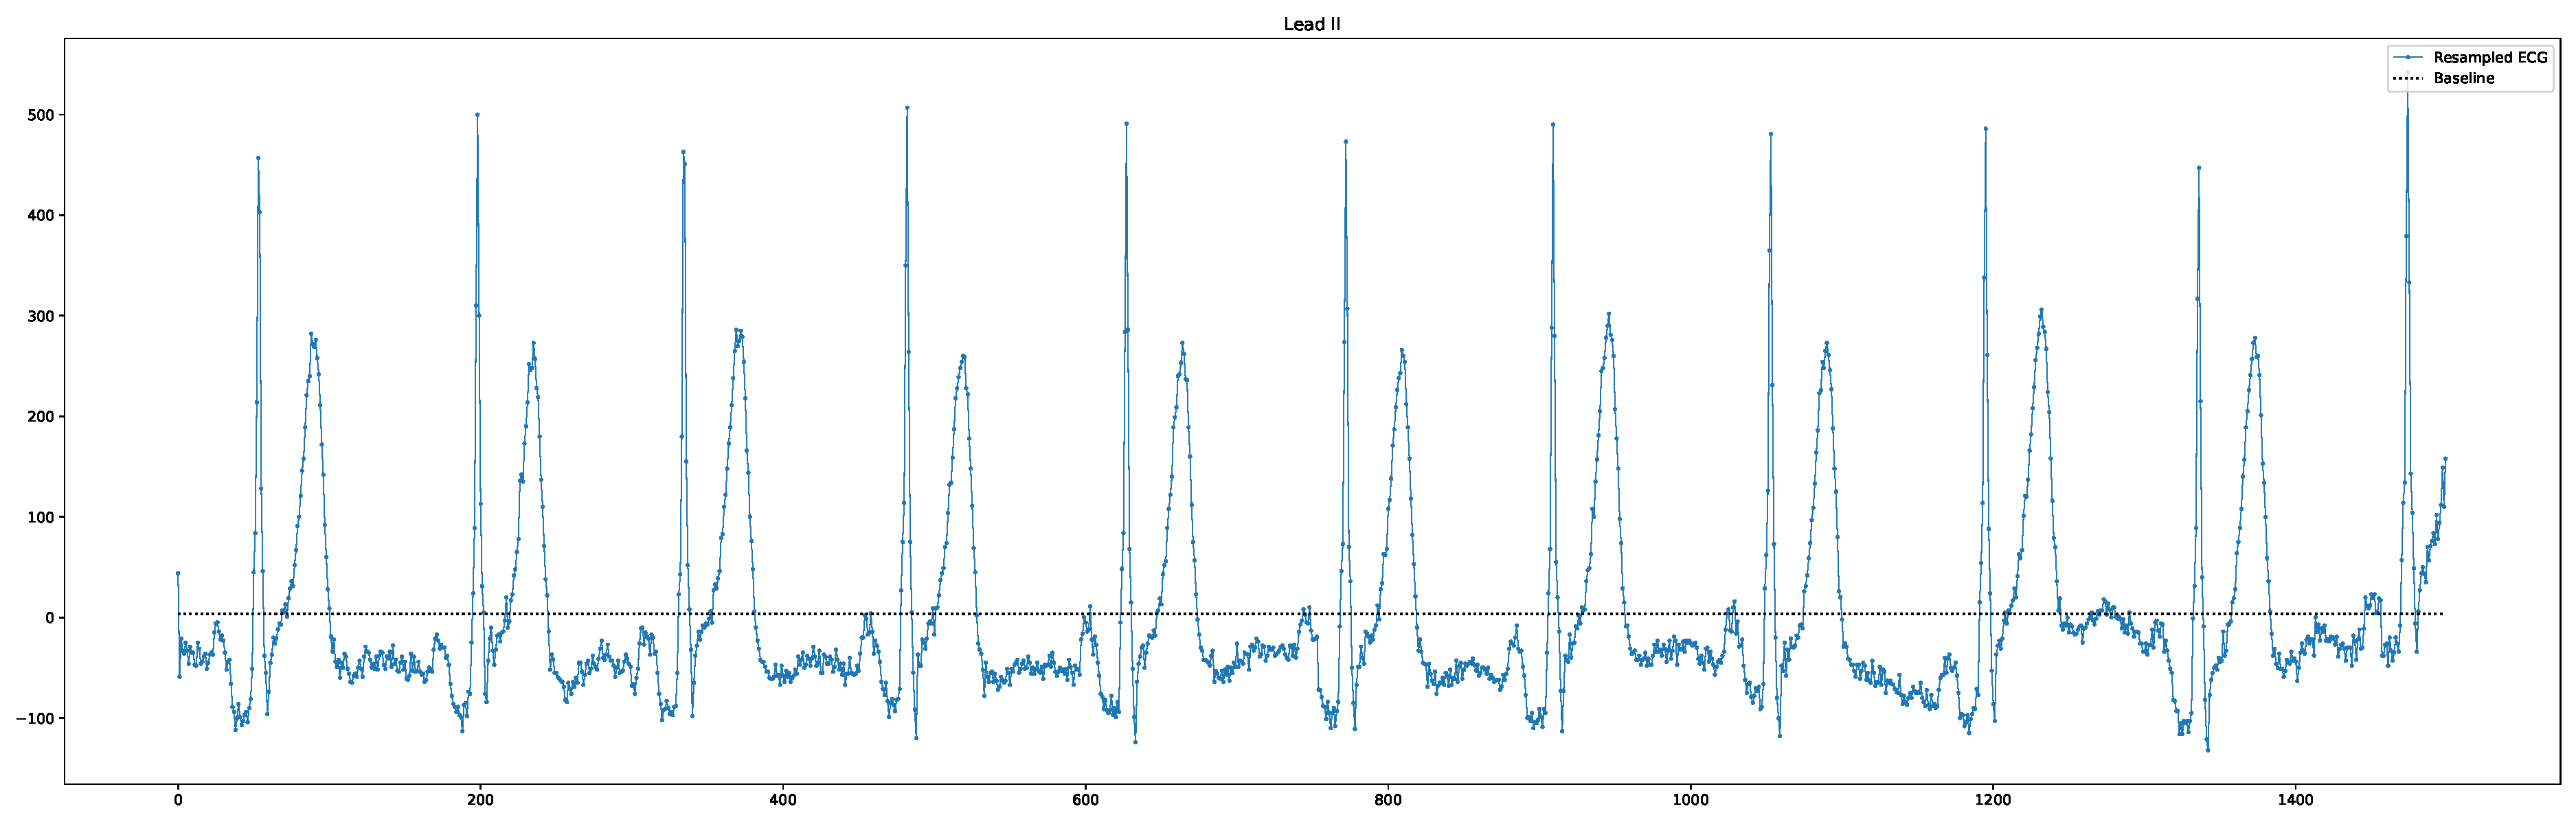
\includegraphics[width=1\linewidth]{images/r_peaks/resampled_ecg_m.pdf}
\caption{Resampled Lead II signal, 1500 points.}
\label{fig:resampled-ecg}
\end{figure}

\noindent After that, the data is denoised via applying wavelet transform. First, the signal is decomposed into wavelet coefficients at different scales using Daubechies wavelet, known for its efficacy in processing signals with sharp peaks and smooth variations, typical of ECG data. The decomposition level is set to the maximum useful level of decomposition, indicating that the signal is decomposed multiple times to extract various frequency components. This step is done using the function \texttt{wavedec} from the Python library \texttt{PyWavelets}. Next, a threshold to differentiate significant signal components from noise is calculated based on the noise level estimated from the smallest scale coefficients, using median absolute deviation to approximate the standard deviation. The coefficients are subjected to soft thresholding, where values below the threshold are set to zero, and values above the threshold are shrunk towards zero. Finally, the denoised signal is reconstructed from the thresholded wavelet coefficients using the inverse wavelet transform. This process effectively removes high-frequency noise components from the ECG signal while preserving the important signal features, resulting in a cleaner and more interpretable signal. After the data is resampled and denoised we also standardise the data. In Figure \ref{fig:res-st-den-ecg} we can see the resampled, denoised, standardised Lead II signal compared to the resampled and standardised Lead II signal. \newline

\begin{figure}[h]
\centering
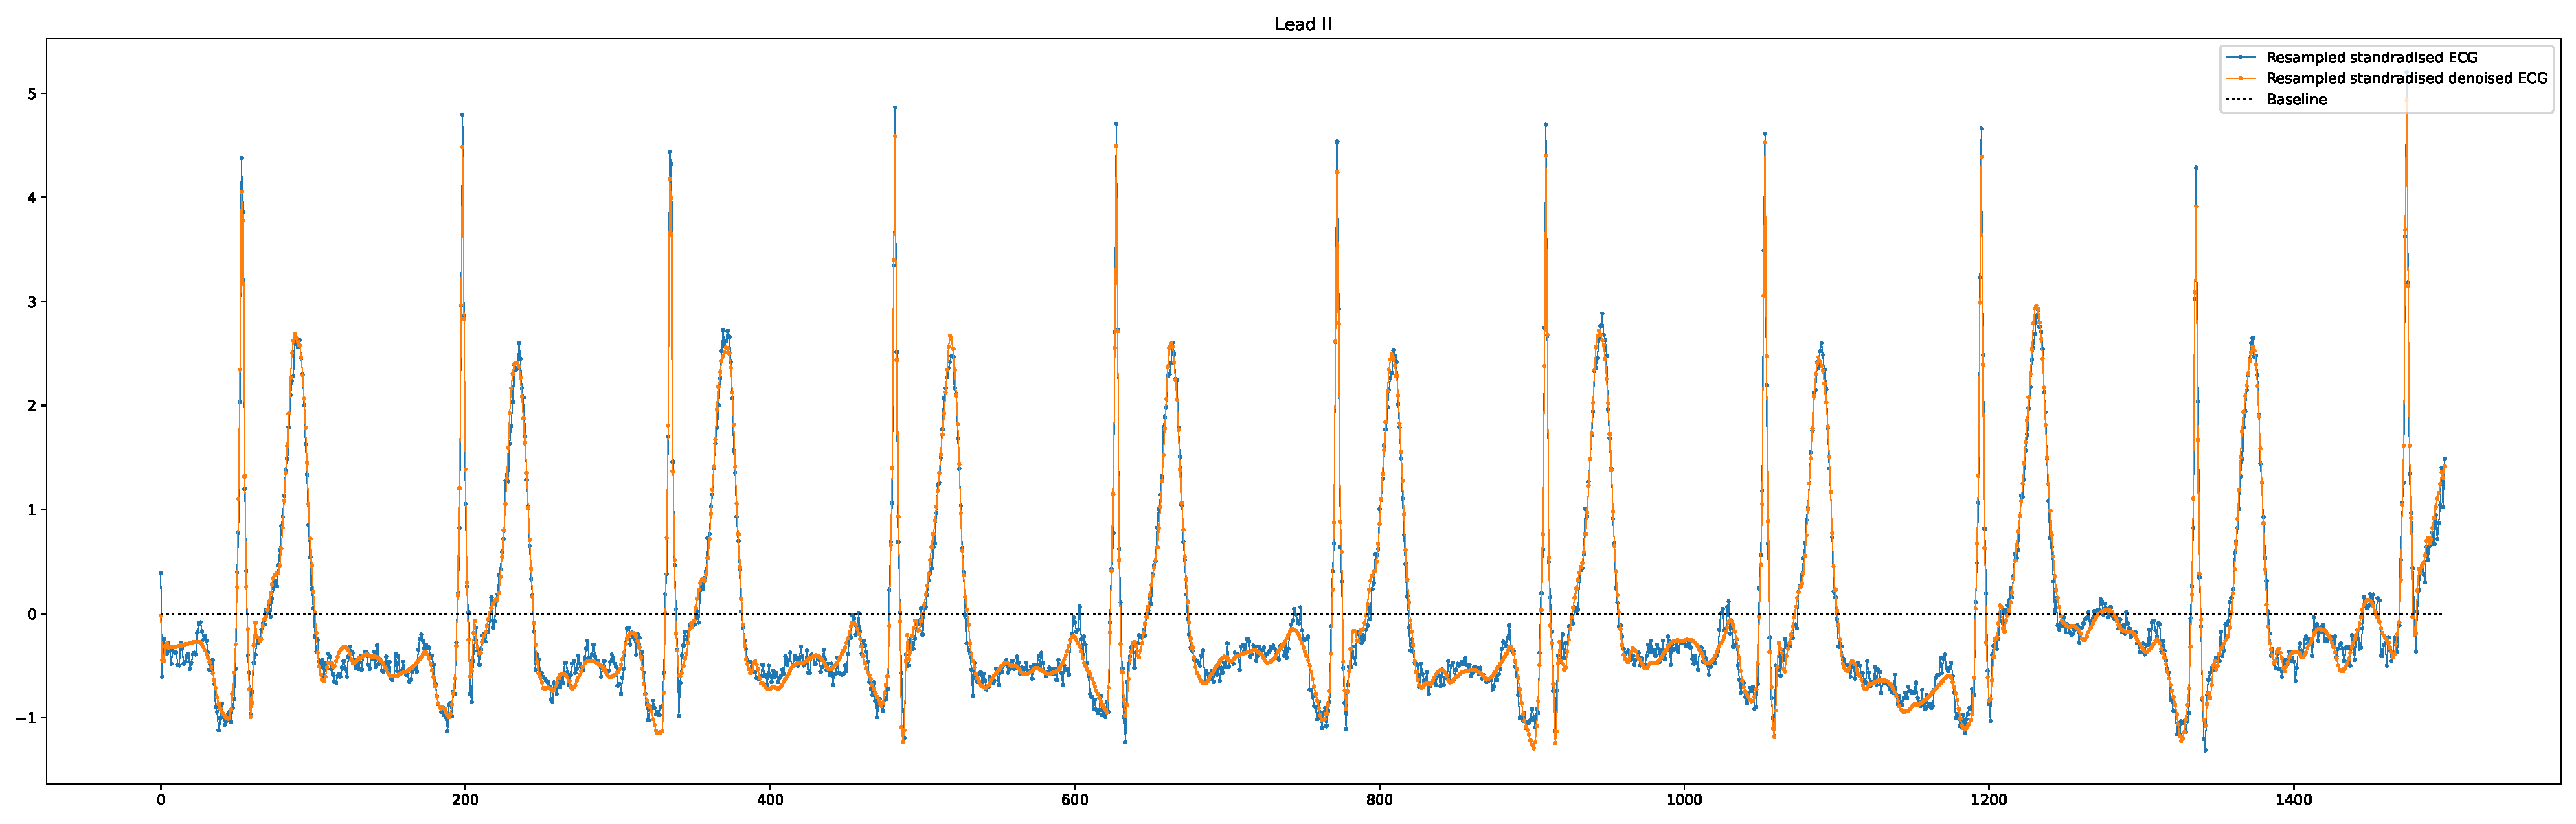
\includegraphics[width=1\linewidth]{images/r_peaks/resampled_standardised_denoised_ecg_m.pdf}
\caption{Resampled and standardised Lead II signal (blue), and the denoised version (orange) of the same signal after applying wavelet transform and standardisation.}
\label{fig:res-st-den-ecg}
\end{figure}

\subsection{PSMF Model}

To summarise, the ECG signal we want to apply PSMF to has $n = 1500$ observations, containing $11$ heart beats, and $m = 12$ variables (corresponding to the $12$ leads introduced in Section \ref{sec:12leads}). To model the subspace with PSMF we choose a periodic subspace model (Fourier basis)
\begin{equation}
    x_k = f_{\theta}(x_{k-1}) = \sum_{i=1}^3 \theta_{1,i} \sin(2\pi \theta_{2,i} k + \theta_{3,i} x_{k-1}) + \theta_{4,i} \cos(2\pi \theta_{5,i} k + \theta_{6,i} x_{k-1}),
\end{equation}
where $\theta_{1,i}, \theta_{4,i} \in \mathbb{R}^{r \times r}$ and $\theta_{2,i}, \theta_{3,i}, \theta_{5,i}, \theta_{6,i} \in \mathbb{R}^{r \times 1}$ for $i = 1, 2, 3$. We also set $r = 3$, $R_k = I_m$, $P_0 = I_r$, $Q_0 = I_r$, $V_0 = v_0 \otimes I_r$ with $v_0 = 5$, and run iterative PSMF with $100$ iterations, and withhold $10\%$ of the data for testing purposes. In Figure \ref{fig:reconstr-ecg} we can see the reconstruction on the training data. It is noticeable that the fit can model the smaller amplitudes, but when it comes to the R wave the amplitude is very low, close to the baseline. Another observation is that the fit is very periodic around the smoother parts which were initially very noisy. Next, we remove the reconstruction from the original data, and choose a threshold as the $99.2$-th percentile of the differences between the reconstruction and the original data. Figure \ref{fig:diff-ecg} visualises the differences (blue) and the chosen threshold line (red). \newline

\begin{figure}[h]
\centering
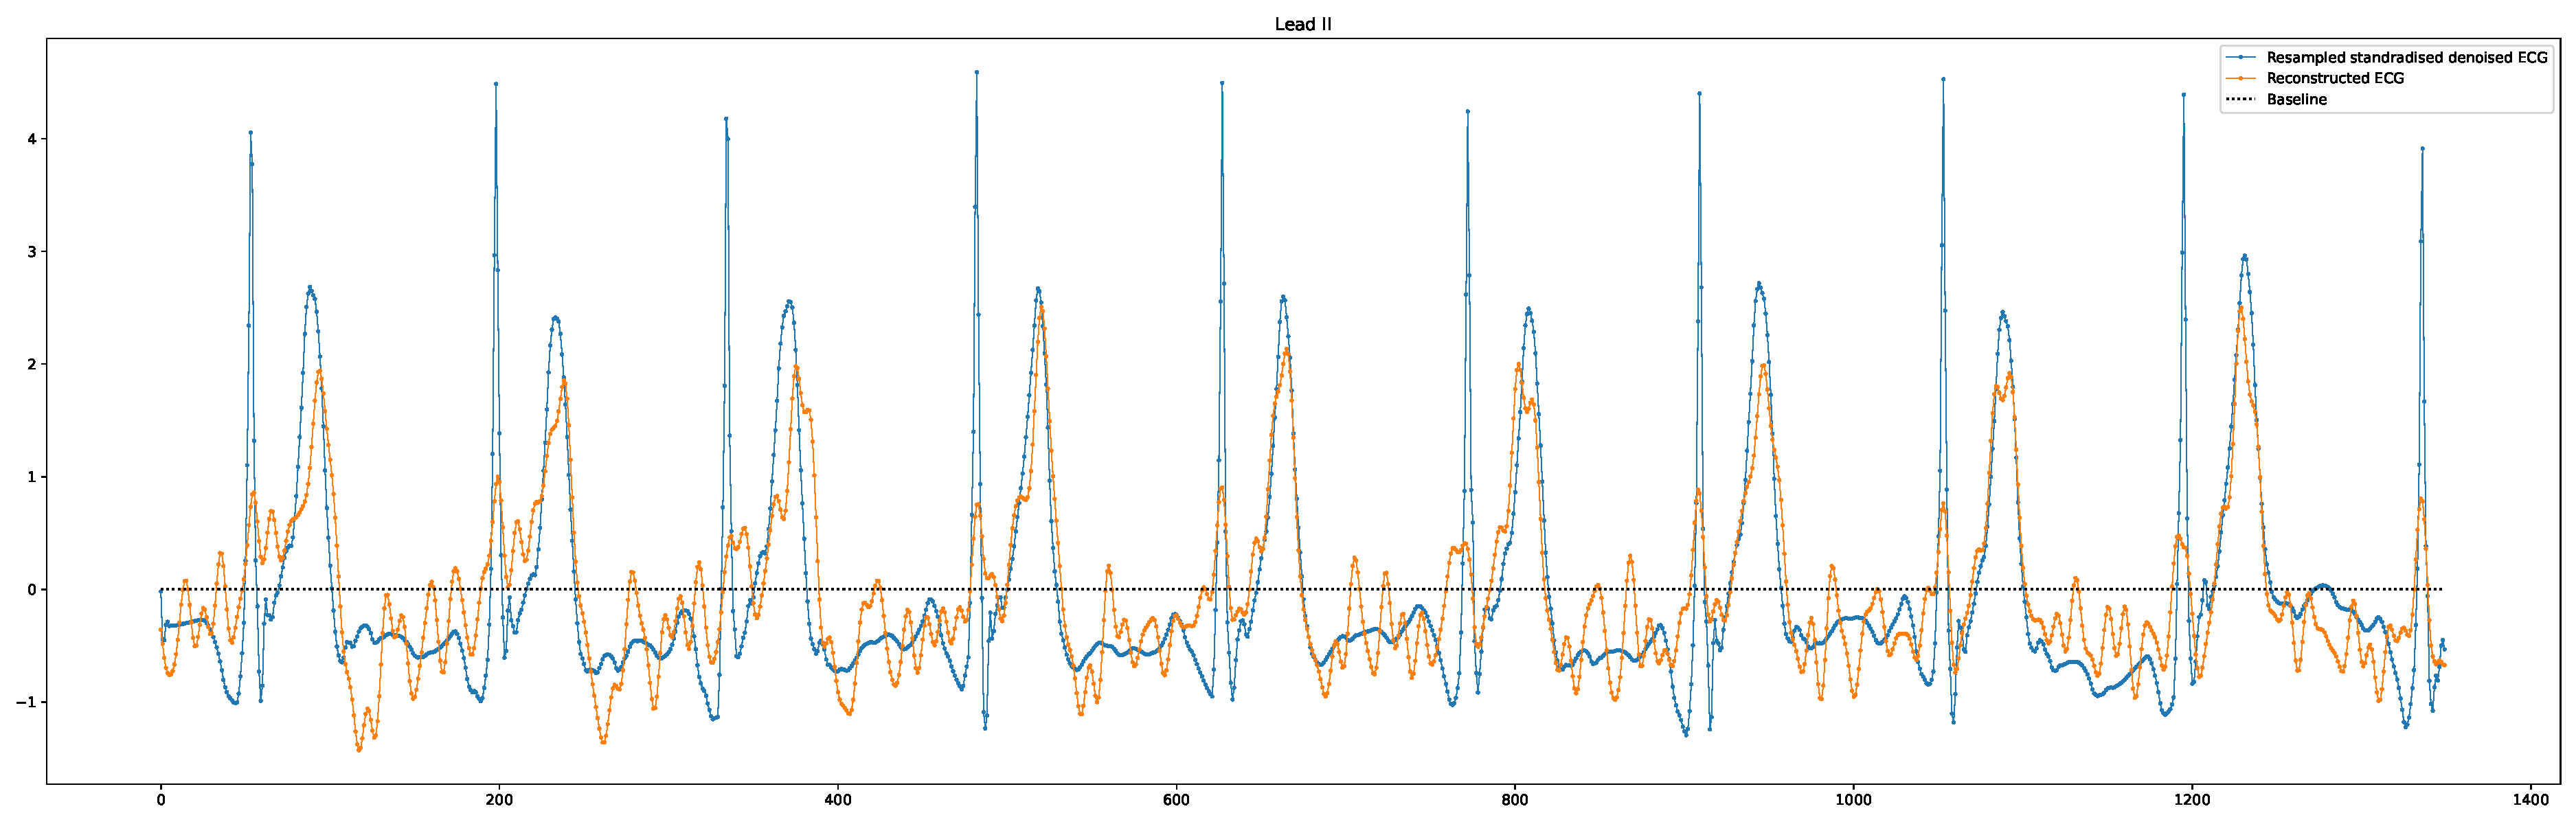
\includegraphics[width=1\linewidth]{images/r_peaks/resampled_standardised_denoised_ecg_reconstruction_m.pdf}
\caption{Lead II signal (blue), and the reconstruction (orange) of the same signal after applying PSMF to the 12 leads with rank $r = 3$, Fourier basis with $n = 3$ terms, and $100$ iterations.}
\label{fig:reconstr-ecg}
\end{figure}

\begin{figure}[h]
\centering
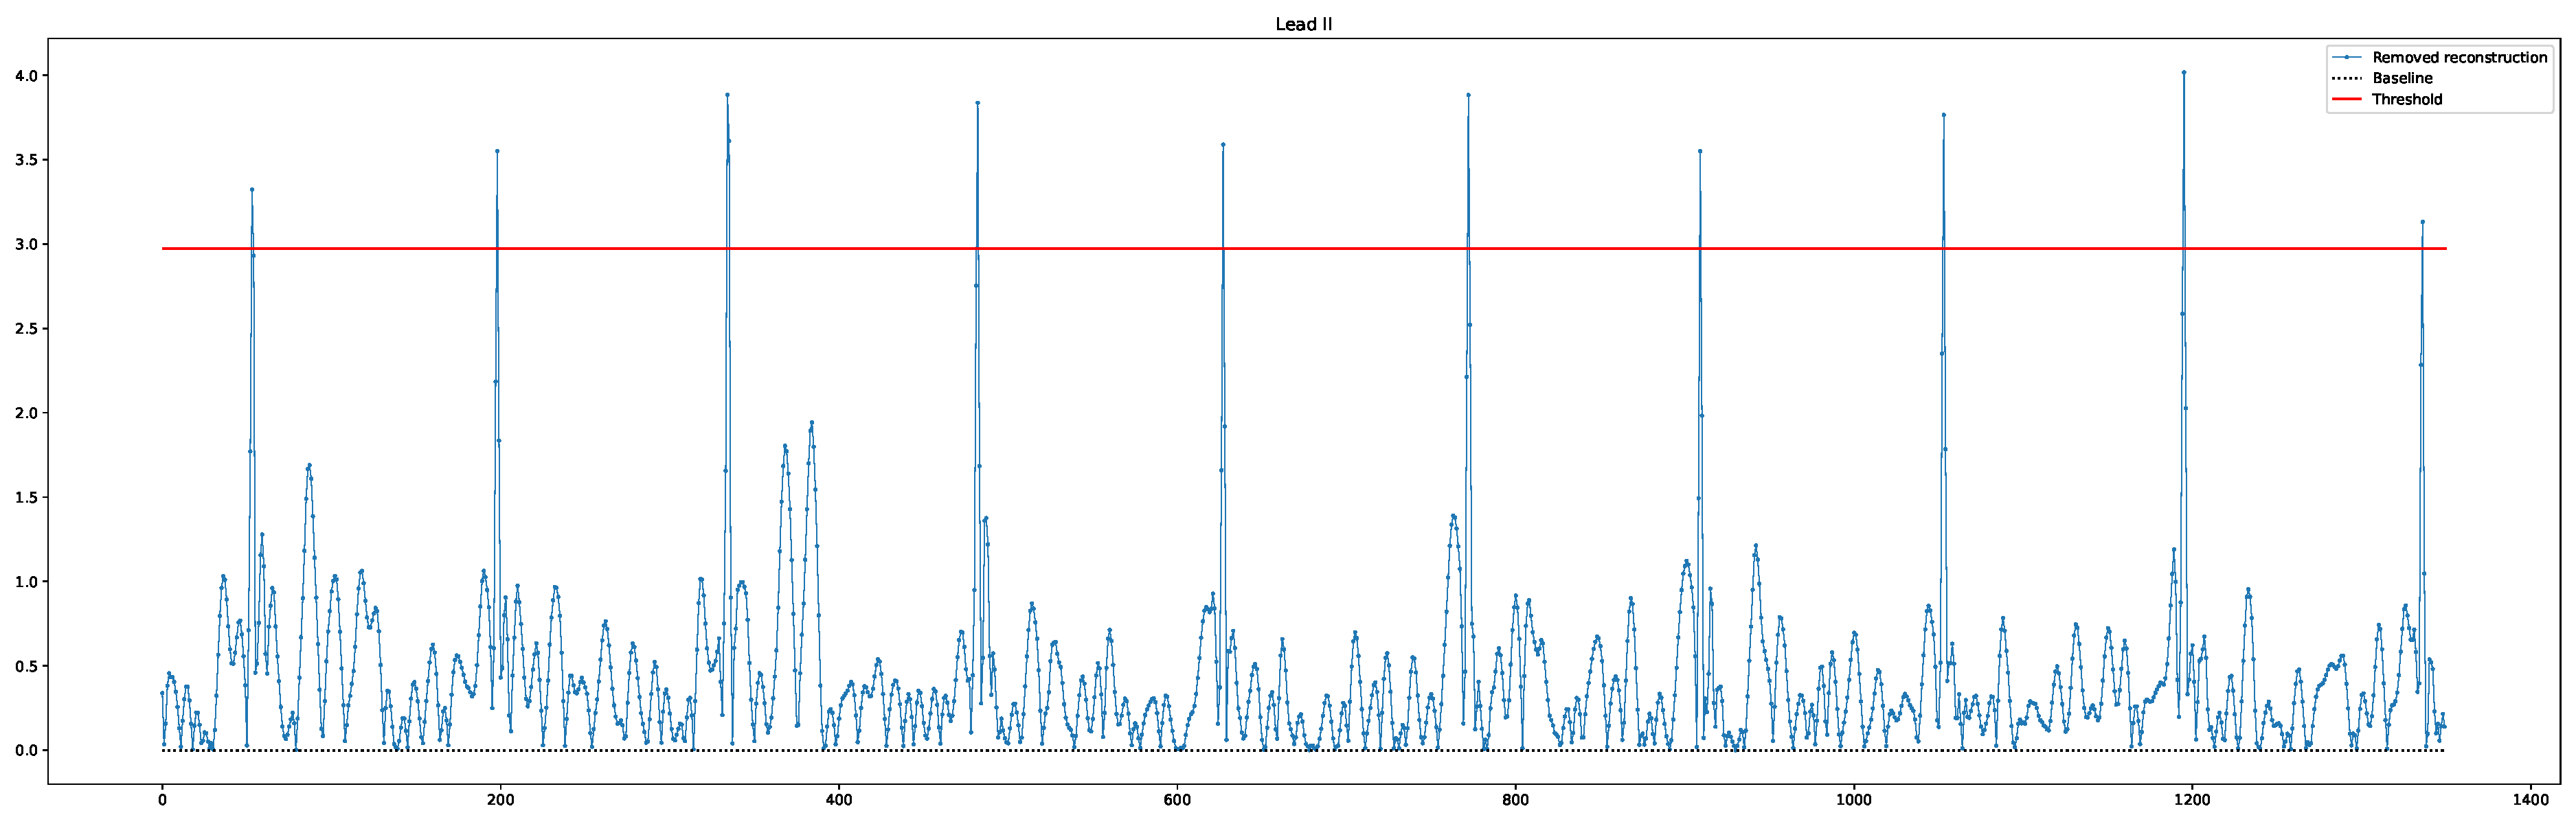
\includegraphics[width=1\linewidth]{images/r_peaks/resampled_standardised_denoised_ecg_rpeaks_algo_m.pdf}
\caption{Removed reconstruction from the modelled ECG signal (blue), and threshold (red) for isolating the R-peaks.}
\label{fig:diff-ecg}
\end{figure}

\noindent Finally, in Figure \ref{fig:rpeaks-ecg} we can see the detected R-peaks (red x) which were chosen as the points above the defined threshold, and the true R-peaks (circle). We can see that the method manages to determine the R-peaks, but in the third heart beat we can see that there is a second point detected as a peak. This is due to the last peak having a noticeably lower amplitude than all of the other peaks, which enforced choosing a lower threshold. This is an example where variable amplitudes might contribute to difficult detection of R-peaks and possibly indicate an issue with the signal such as artifacts, poor electrode contact, etc. This highlights the potential impact of variable amplitudes on R-peak detection and the need for robust methods to handle such variations. \newline

\begin{figure}[h]
\centering
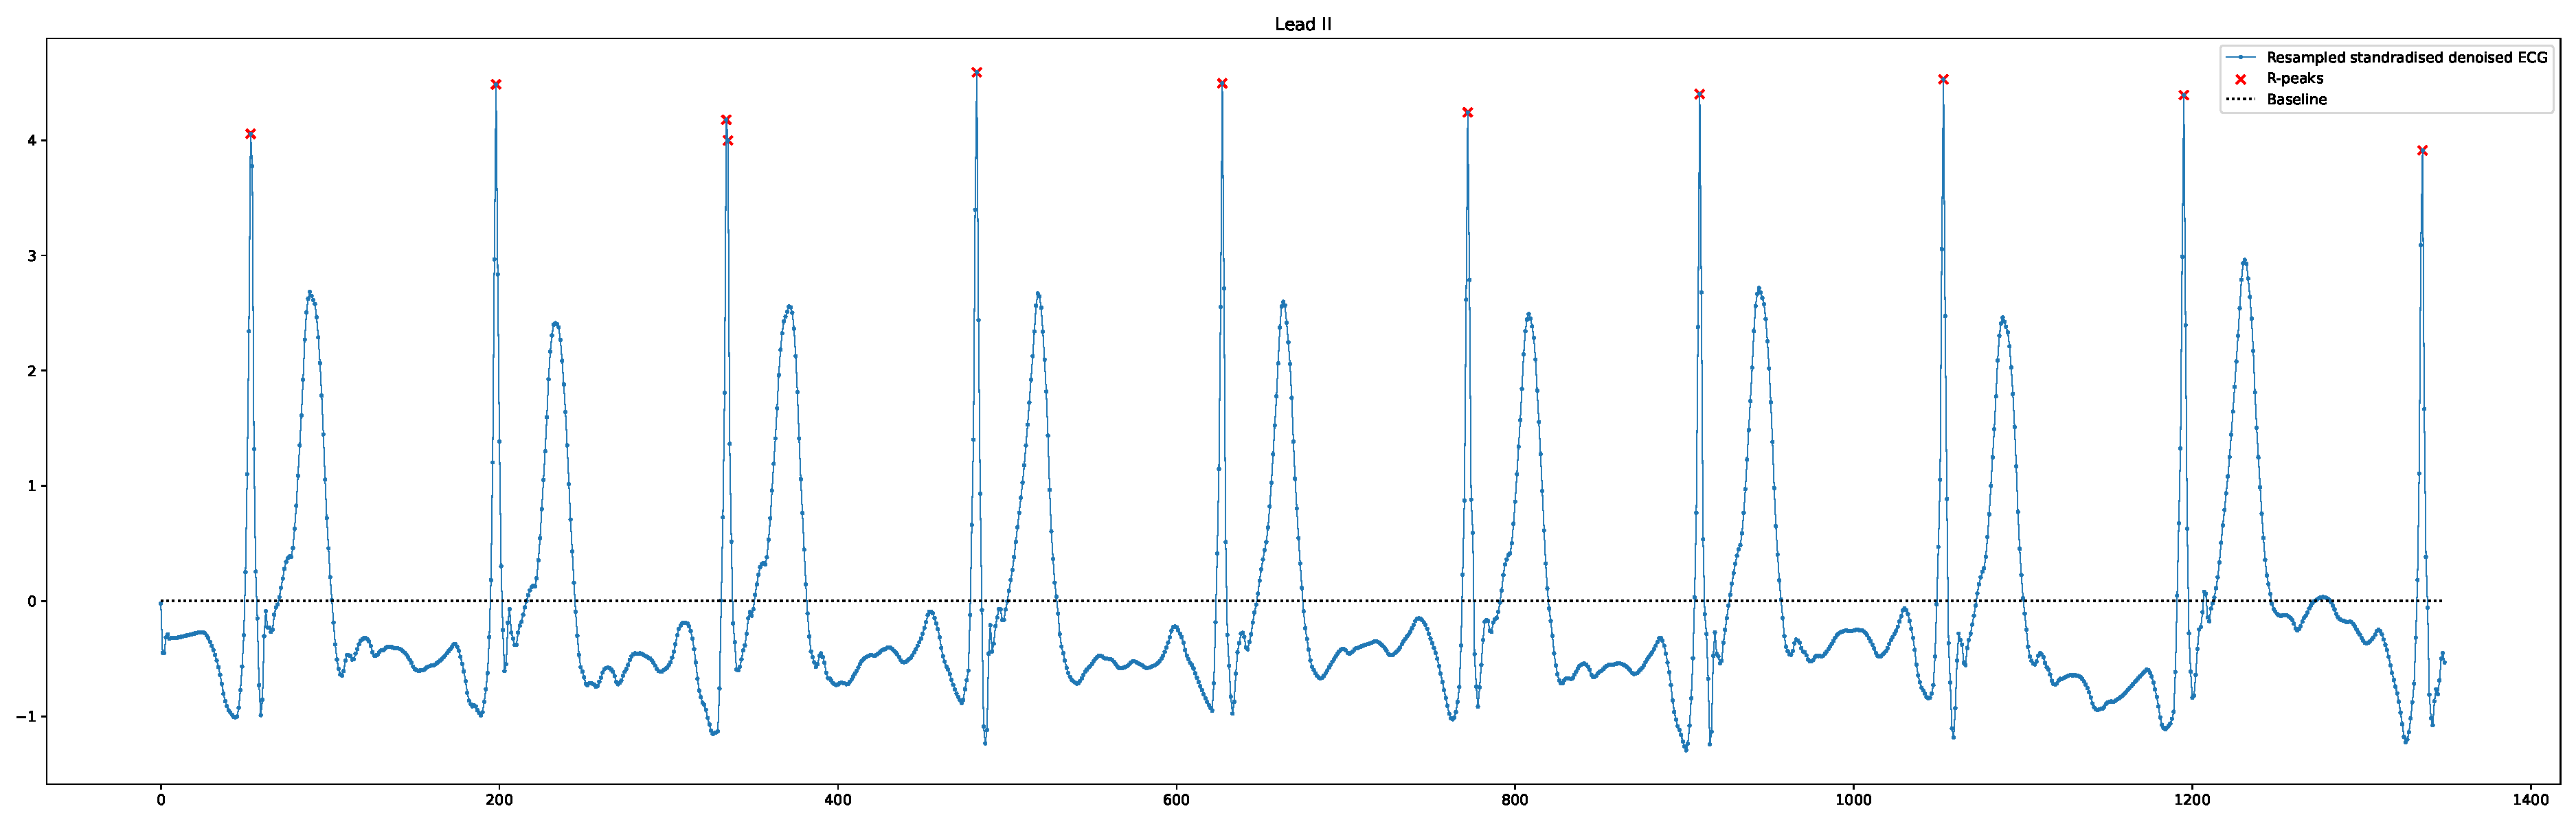
\includegraphics[width=1\linewidth]{images/r_peaks/resampled_standardised_denoised_ecg_rpeaks_m.pdf}
\caption{Detected R-peaks (red x) and the true R-peaks (circle) in the resampled, standardised, denoised Lead II signal (blue).}
\label{fig:rpeaks-ecg}
\end{figure}

\subsection{Conclusion}

\noindent In conclusion, the novel R-peak detection method presented in this section effectively harnesses the predictive discrepancies inherent to the PSMF model as a feature rather than a drawback. By deliberately using a model that underestimates the amplitude of R-peaks, we create a predictable deviation from the original ECG signal, which can then be quantitatively identified using a threshold-based approach. Our empirical results demonstrate that this method can reliably detect R-peaks within a resampled, standardized, and denoised ECG signal, Lead II in particular. The method maintains the integrity of critical signal features after substantial data manipulation including resampling and noise reduction. Further refinements may be necessary to address outliers and ensure universal applicability across different types of ECG signals and conditions.

\section{Forecasting}

In this section we are going to show our attempt at forecasting 12-lead ECG data with PSMF. We apply the algorithm to 12-lead ECG data containing $2$ whole heart beats, and attempt to make a forecast for the future ECG behaviour.

\subsection{Data}

The data used and the preprocessing is the same as the one described in Section \ref{sec:rpeaksdet}, with the only difference that this time we are going to use only $400$ data points, corresponding to $3$ heart beats from the ECG.

\subsection{PSMF Model}\label{exp3:psmfmodel}

The ECG signal we want to apply PSMF to has $n = 400$ observations, containing $3$ heart beats, and $m = 12$ variables (corresponding to the $12$ leads introduced in Section \ref{sec:12leads}). To model the subspace with PSMF we choose a Fourier basis with $n = 3$ terms
\begin{equation}
    x_k = f_{\theta}(x_{k-1}) = \sum_{i=1}^3 \theta_{1,i} \sin(2\pi \theta_{2,i} k + \theta_{3,i} x_{k-1}) + \theta_{4,i} \cos(2\pi \theta_{5,i} k + \theta_{6,i} x_{k-1}),
\end{equation}
where $\theta_{1,i}, \theta_{4,i} \in \mathbb{R}^{r \times r}$ and $\theta_{2,i}, \theta_{3,i}, \theta_{5,i}, \theta_{6,i} \in \mathbb{R}^{r \times 1}$ for $i = 1, 2, 3$. We also set $r = 6$, $R_k = I_m$, $P_0 = I_r$, $Q_0 = I_r$, $V_0 = v_0 \otimes I_r$ with $v_0 = 5$, and run iterative PSMF with $400$ iterations, and withhold $20\%$ of the data for prediction. In other words, we use an observed time series of length $320$ (corresponding to $2$ heart beats) and a series of unobserved future data of length $80$ (corresponding to approximately $1$ heart beat). \newline

\subsection{Results}

\noindent In Figure \ref{forecast} we can see the PSMF fitting on 12-lead ECG data with rank $r = 6$, $n = 3$ Fourier terms, over $400$ iterations. The observed time series is shown in blue, the unobserved future data is shown in yellow, and the reconstruction from the model is shown in red. We can see, as mentioned in Section \ref{sec:rpeaksdet}, that the model has a hard time with modelling the high amplitudes. This also affects the forecast, although we can see that the prediction stays in reasonable bounds and manages to follow the dynamics of the signal. If we refer to Figure \ref{problem} we can notice that the high amplitudes with sharp peaks corresponding mainly to the R waves are described by significantly less points compared to the other waves from the PQRST complex. This is due to the R wave representing the rapid depolarization of the ventricles, particularly the left ventricle. This quick process creates a sharp, narrow spike on the ECG with high amplitude but short duration, requiring fewer points to capture it compared to slower waves like the P or T waves. These fewer points in the part towards the peak might be considered by the PSMF as outliers, or it might just be the case that the ECG data is too complex for the PSMF model. \newline

\begin{figure}[h]
\begin{center}
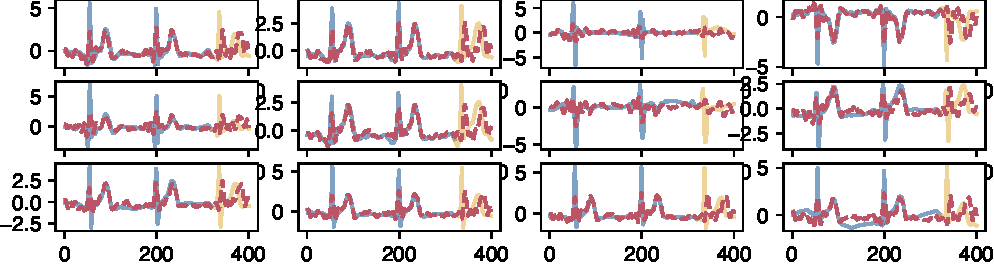
\includegraphics[scale=1]{images/forecast/periodic_fit.pdf}
\caption{Fitting PSMF on 12-lead ECG data with rank $r = 6$, $n = 3$ Fourier terms, $400$ iterations. Observed time series (blue) with unobserved future data (yellow) and the reconstruction from the model (red).}
\label{forecast}
\end{center}
\end{figure}

\begin{figure}[h]
\begin{center}
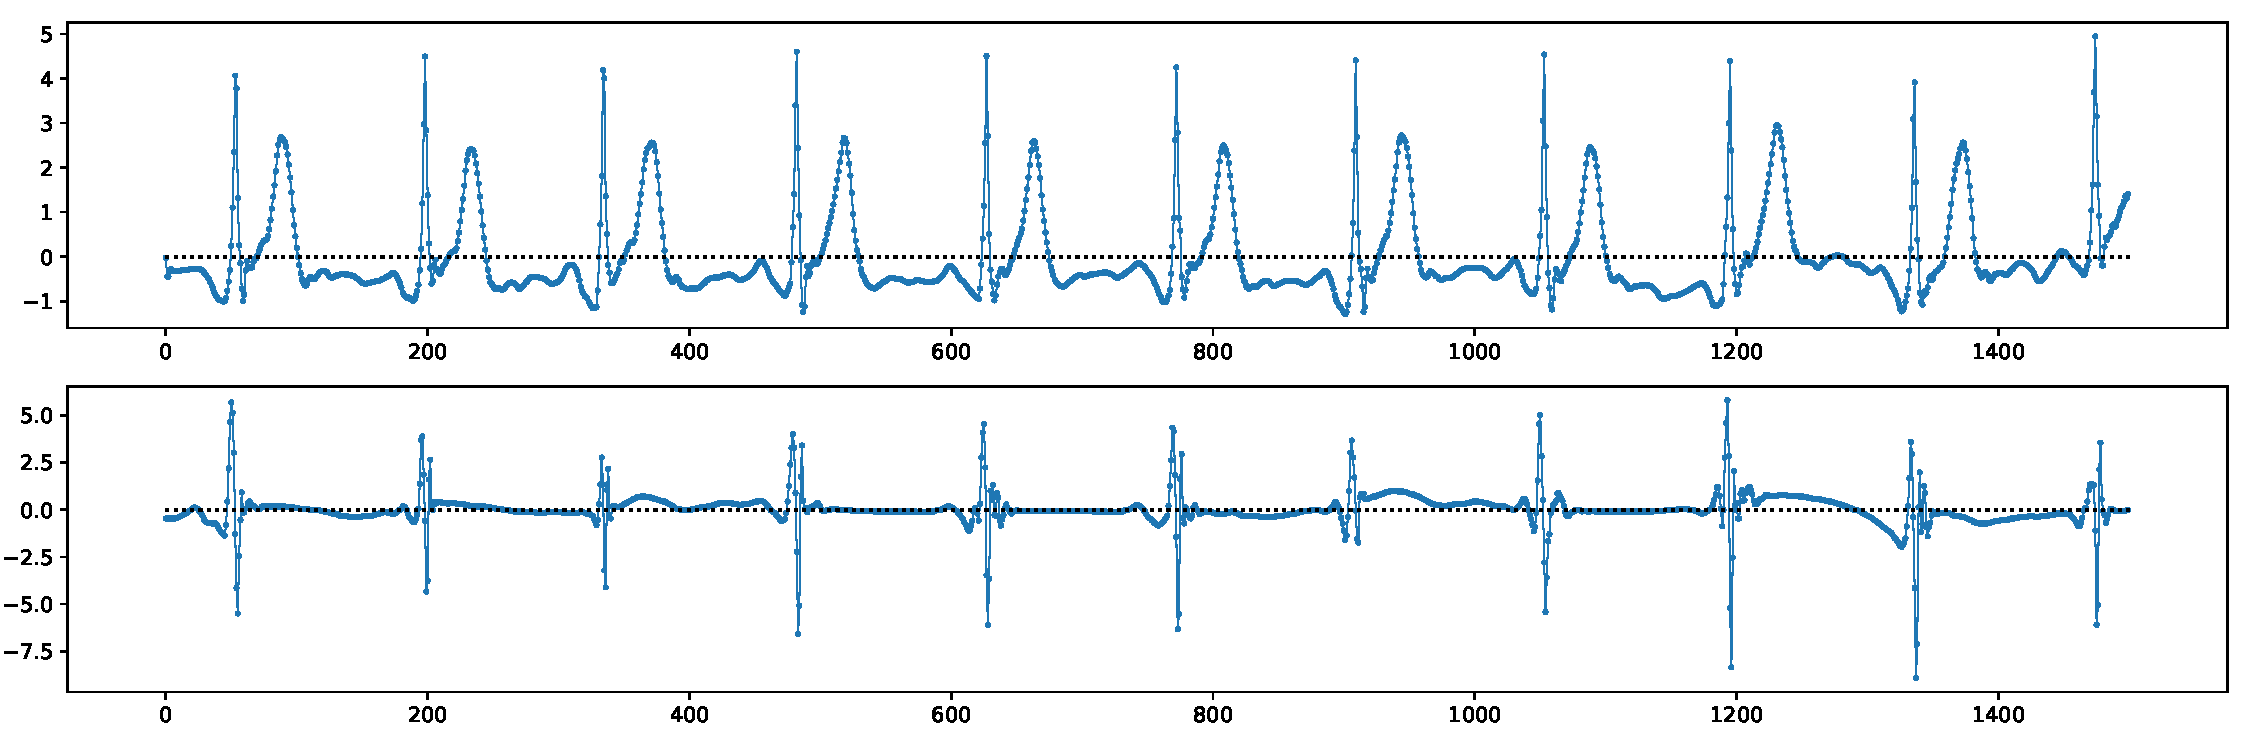
\includegraphics[scale=0.4]{images/example.pdf}
\caption{A visualisation of the high sharp-peak amplitudes being described by fewer data points compared to the other waves.}
\label{problem}
\end{center}
\end{figure}

\begin{figure}[h]
\begin{center}
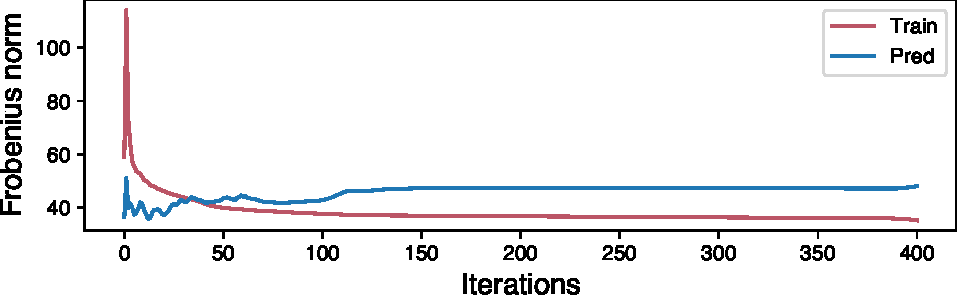
\includegraphics[scale=1]{images/forecast/periodic_cost.pdf}
\caption{Reconstruction error $\Vert Y - CX \Vert^2_F$ for the observed data (red) and the unobserved future data (blue).}
\label{loss}
\end{center}
\end{figure}

\noindent Figure \ref{loss} shows how the Frobenius norm $\Vert Y - CX \Vert^2_F$ between the reconstructed data and the true data behaves with the number of iterations. The training loss starts very high but rapidly decreases in the first few iterations, stabilizing around a lower value by approximately $50$ iterations. This indicates that the model is quickly learning to fit the training data. After the initial drop, the training loss continues to decrease gradually but remains relatively stable, indicating that the model has reached a point where additional iterations yield only marginal improvements. The prediction loss is initially lower than the training loss but shows more fluctuation. After about $50$ iterations, it starts to stabilize as well, though it remains consistently higher than the training loss. This gap between the training and prediction loss suggests that the model may be overfitting the training data, as it performs better on the training set than on the prediction task. Experimenting with stopping the training earlier resulted in predictions which had worse wave amplitudes and were shifted compared to the original data. Finally, Figure \ref{bases} shows how the underlying subspace is recovered. \newline

\begin{figure}[h]
\begin{center}
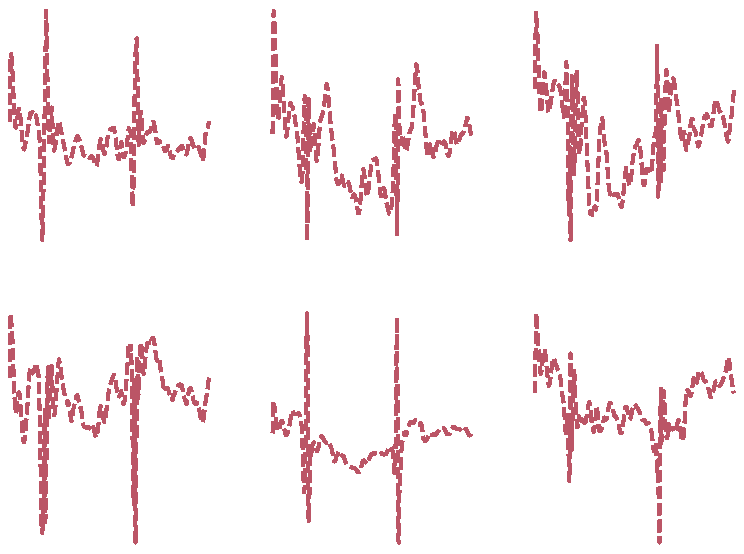
\includegraphics[scale=0.6]{images/forecast/periodic_bases.pdf}
\caption{Recovered subspace.}
\label{bases}
\end{center}
\end{figure}

\subsection{Conclusion}

\noindent In this section, we applied PSMF trained on two heartbeats to forecast a 12-lead ECG signal. The results showed that while the model could reasonably follow the dynamics of the ECG signal, it struggled with accurately capturing high-amplitude sharp peaks, particularly the R waves. The training and prediction loss analysis indicated that the model might be overfitting, as it performed better on the training data than on the unobserved future data. Despite these challenges, the PSMF model maintained predictions within reasonable bounds, though with some limitations in amplitude accuracy and timing.

\chapter{Conclusion}

In this thesis, we presented novel applications of the probabilistic sequential matrix factorization (PSMF) algorithm to 12-lead ECG data. Our goal was to explore the potential of PSMF in addressing tasks related to this complex, high-dimensional time-series data with nonlinear subspace. \newline

\noindent We began by introducing the PSMF model and its robust variant, rPSMF, along with the relevant mathematical framework. We also outlined the inference process, parameter estimation techniques, and the algorithms for both PSMF and rPSMF. Additionally, we discussed the adaptation of PSMF for handling missing data in ECG signals. \newline

\noindent In Chapter 3, we demonstrated three applications of PSMF to 12-lead ECG data:
\begin{itemize}
    \item \textbf{Missing data imputation:} We applied both PSMF and rPSMF to impute missing data in ECG signals and compared their performance with other probabilistic sequential matrix factorization algorithms. Our results showed that PSMF and rPSMF generally outperformed the baseline methods, particularly at lower matrix ranks. We also concluded that PSMF and rPSMF perform better when the rank is lower.
    \item \textbf{R-peak detection:} We introduced a novel approach for R-peak detection by leveraging the discrepancy between the original ECG signal and the PSMF reconstruction. By removing the smoother reconstructed signal from the original data and applying a suitable threshold, we successfully identified R-peaks in the ECG signal.
    \item \textbf{Forecasting:} We attempted to forecast an ECG component based on previous normal heartbeats by incorporating a Fourier basis with multiple terms and rank higher than one. While the PSMF model captured the general dynamics of the ECG signal, it faced challenges in accurately modeling the high-amplitude, sharp peaks associated with R waves.
\end{itemize}
Our experiments, conducted on a comprehensive, high-quality 12-lead ECG dataset, demonstrated the potential of PSMF in handling complex ECG data. However, we also identified limitations and challenges, particularly in forecasting tasks involving rapid depolarization events like R waves. \newline

\noindent In conclusion, this thesis highlights the applicability of PSMF to real-world ECG data and its effectiveness in tasks such as missing data imputation and R-peak detection. However, further research is needed to refine the model and improve its performance in forecasting complex ECG features. Future work could focus on model enhancements, probabilistic extensions, alternative inference techniques, and real-time applications to fully harness the potential of PSMF in ECG analysis and monitoring.

\section{Future work}

Given the findings of this thesis, one promising direction is to refine the PSMF model to better handle the sharp, high-amplitude peaks in ECG signals, particularly the R waves. This could involve modifying the periodic subspace model to account for rapid depolarization events more effectively. If this cannot be achieved, the PSMF model can be further extended by adopting different likelihoods and different dynamics which can better capture such complex signal dynamics. Another possibility is to work on enhancing the computational efficiency, and provide new computational tools for inference. In summary, future research efforts should focus on refining the PSMF model to better capture the complexities of ECG signals, exploring probabilistic extensions and alternative inference techniques, and transitioning the model to real-time applications. By addressing these challenges and expanding the scope of PSMF's application, we can unlock its full potential in ECG analysis and beyond, ultimately contributing to improved cardiac monitoring and patient care.

\clearpage
 %% reset page counter and start appendix pages with A
\pagenumbering{arabic}
\renewcommand*{\thepage}{A\arabic{page}}

%%References part of appendices
% References: modify the file refs.bib
\bibliographystyle{plainnat}
\bibliography{refs}

%% Appendix goes here
\appendix

\chapter{Missing Data Imputation Results}\label{app:mdi}

Full results of testing on the $20\%$, $30\%$, and $40\%$ missing data with both $r = 3$ and $r = 10$.

\section{PSMF}

\subsection{$r = 3$}

\begin{figure}[H]
\centering
% First row
\begin{minipage}{0.3\linewidth}
    \centering
    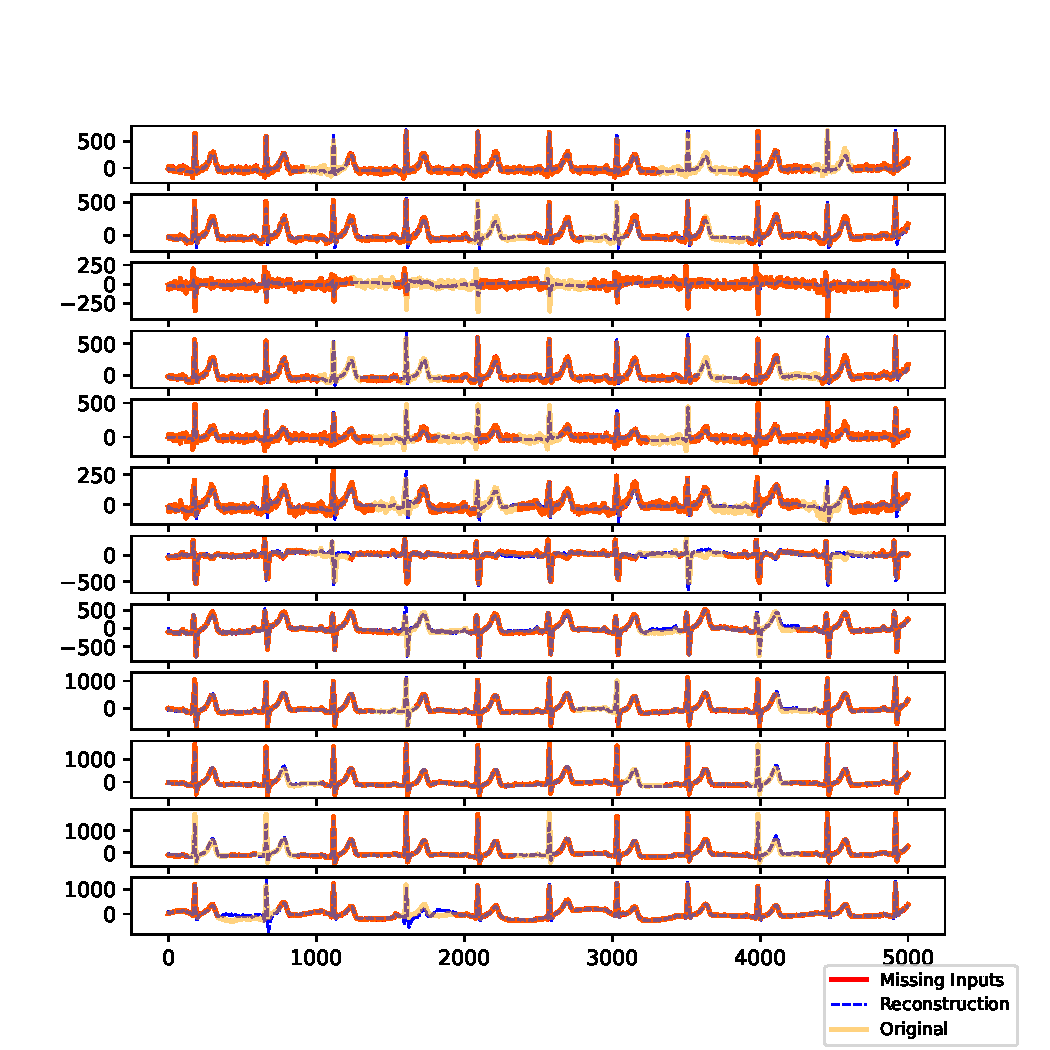
\includegraphics[width=\linewidth]{images/missing/psmf_output_20_3.pdf}
    \caption{$20\%$ missing data.}
\end{minipage}%
\hspace{0.05\linewidth}
\begin{minipage}{0.3\linewidth}
    \centering
    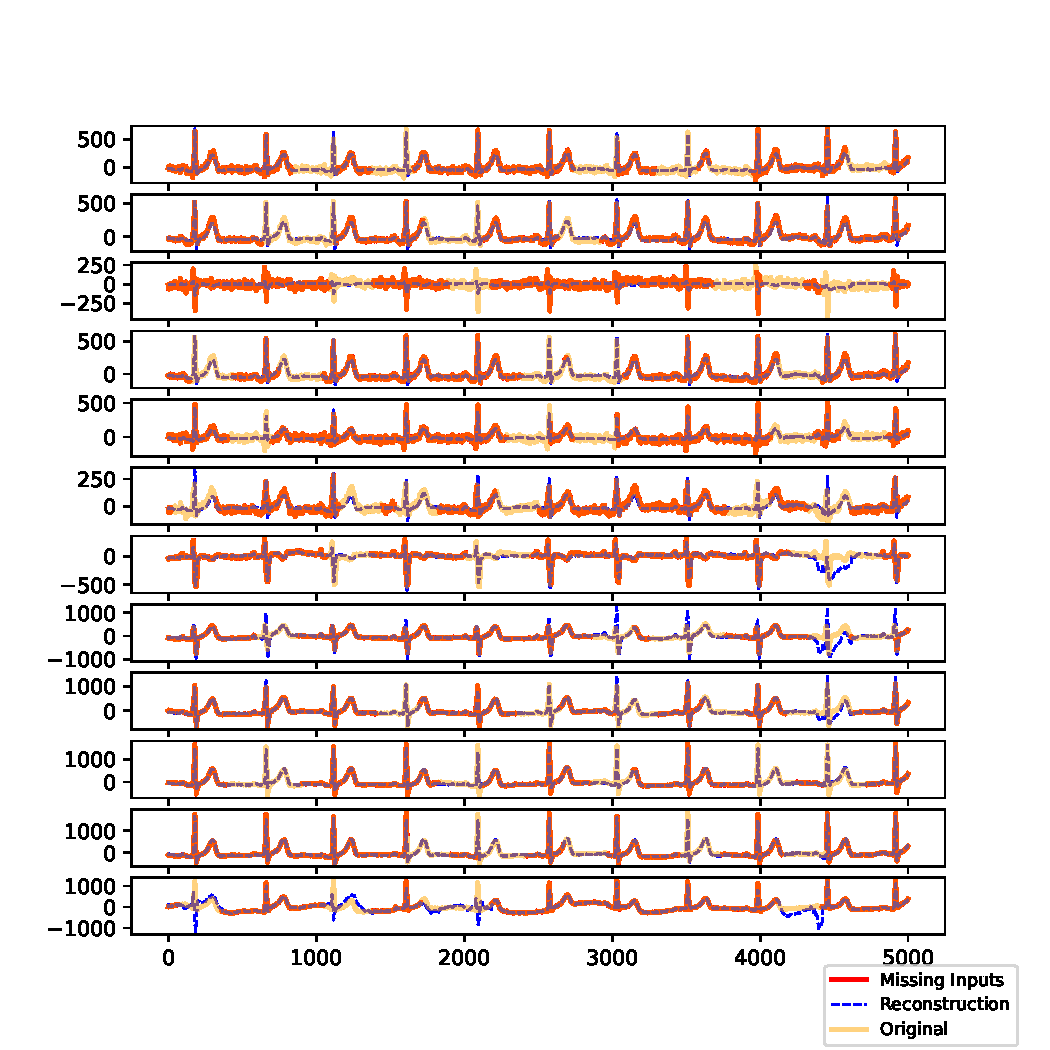
\includegraphics[width=\linewidth]{images/missing/psmf_output_30_3.pdf}
    \caption{$30\%$ missing data.}
\end{minipage}

\vspace{1em} % Adjust vertical space between the rows if necessary

% Second row
\begin{minipage}{0.3\linewidth}
    \centering
    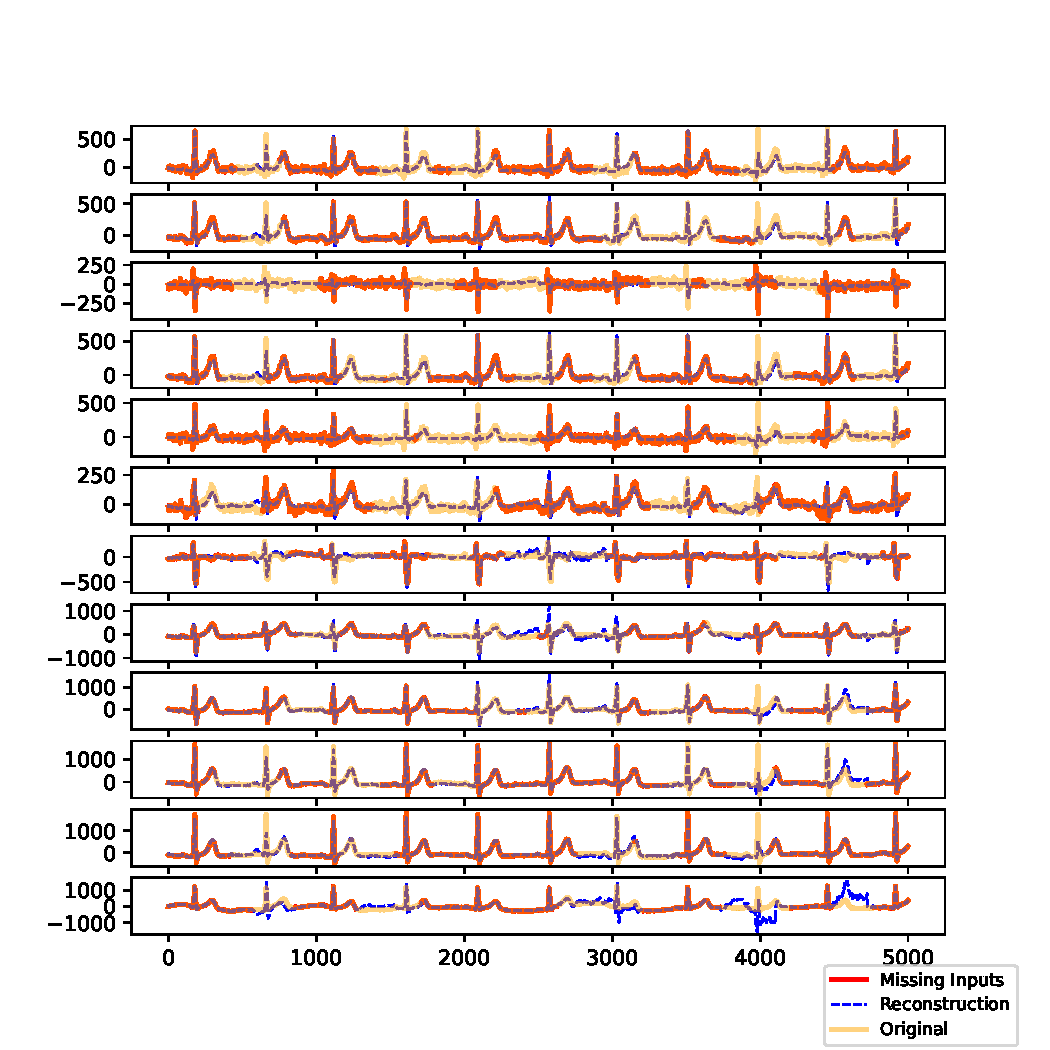
\includegraphics[width=\linewidth]{images/missing/psmf_output_40_3.pdf}
    \caption{$40\%$ missing data.}
\end{minipage}
\end{figure}

\subsection{$r = 10$}

\begin{figure}[H]
\centering
% First row
\begin{minipage}{0.4\linewidth}
    \centering
    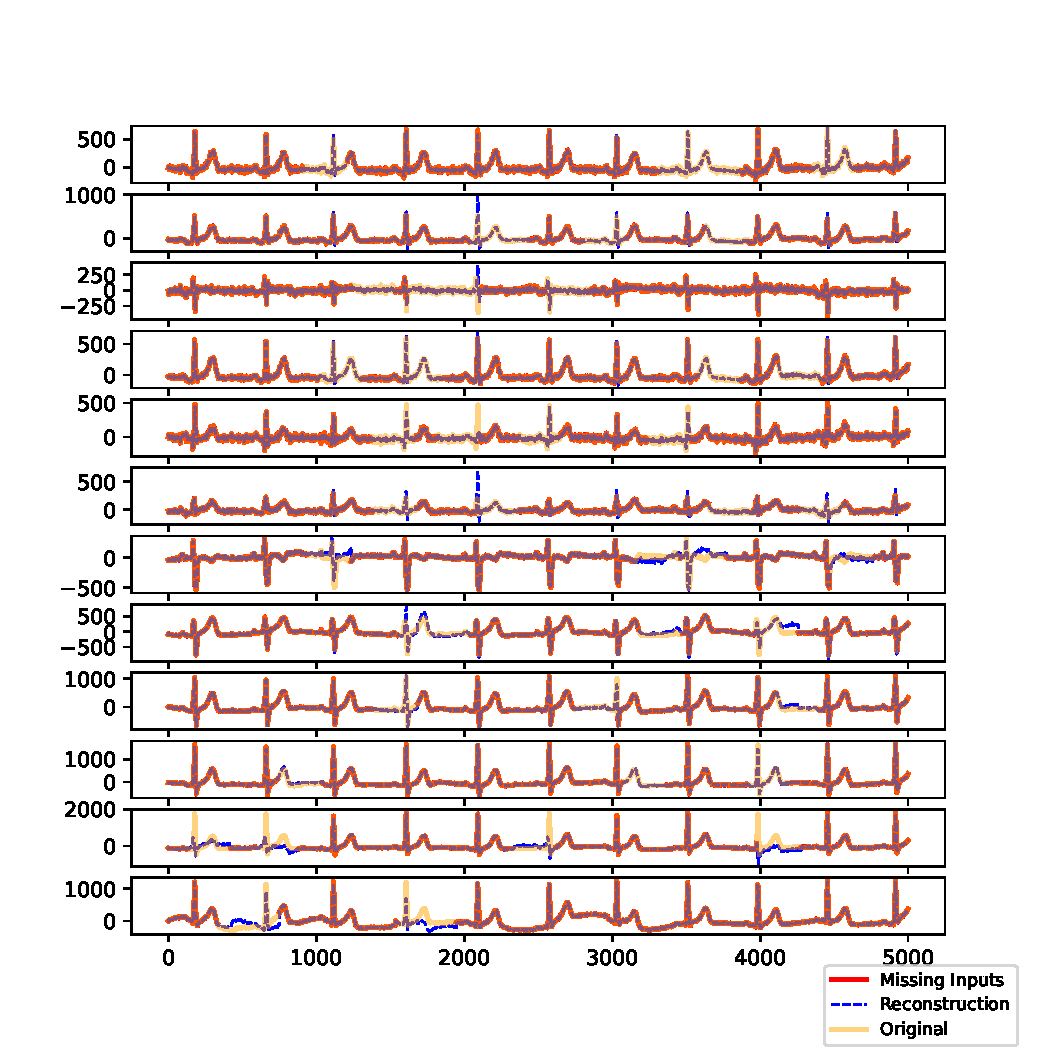
\includegraphics[width=\linewidth]{images/missing/psmf_output_20_10.pdf}
    \caption{$20\%$ missing data.}
\end{minipage}%
\hspace{0.05\linewidth}
\begin{minipage}{0.4\linewidth}
    \centering
    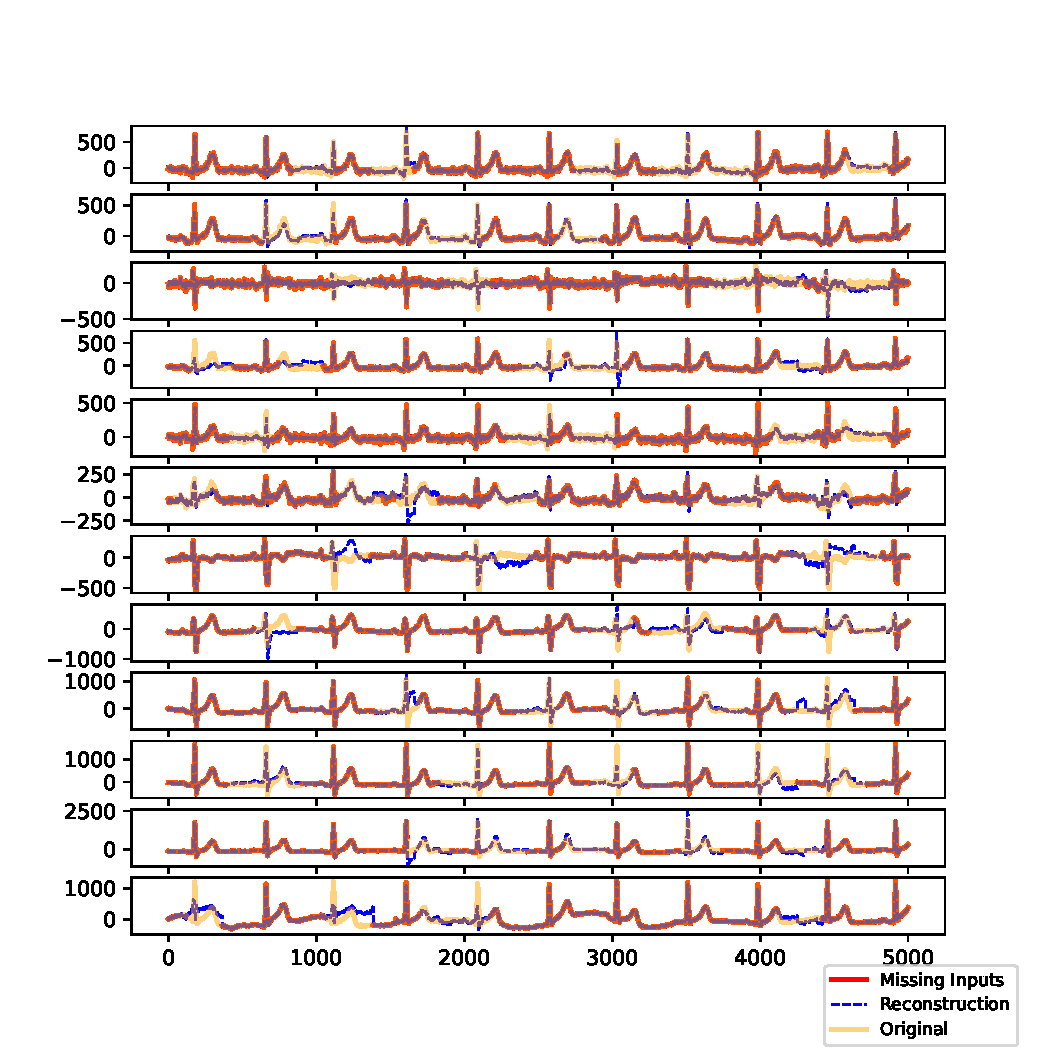
\includegraphics[width=\linewidth]{images/missing/psmf_output_30_10.pdf}
    \caption{$30\%$ missing data.}
\end{minipage}

\vspace{1em} % Adjust vertical space between the rows if necessary

% Second row
\begin{minipage}{0.4\linewidth}
    \centering
    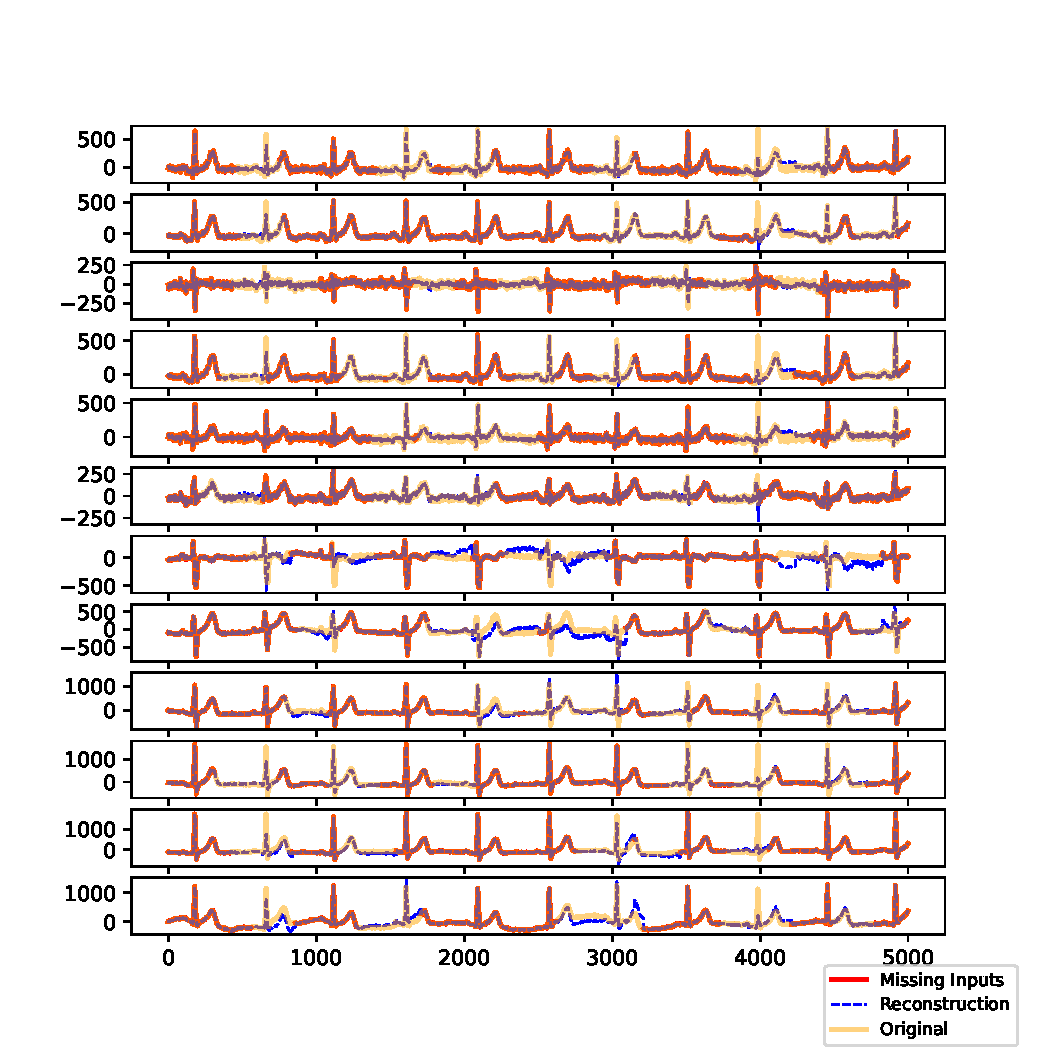
\includegraphics[width=\linewidth]{images/missing/psmf_output_40_10.pdf}
    \caption{$40\%$ missing data.}
\end{minipage}
\end{figure}

\section{rPSMF}

\subsection{$r = 3$}

\begin{figure}[H]
\centering
% First row
\begin{minipage}{0.4\linewidth}
    \centering
    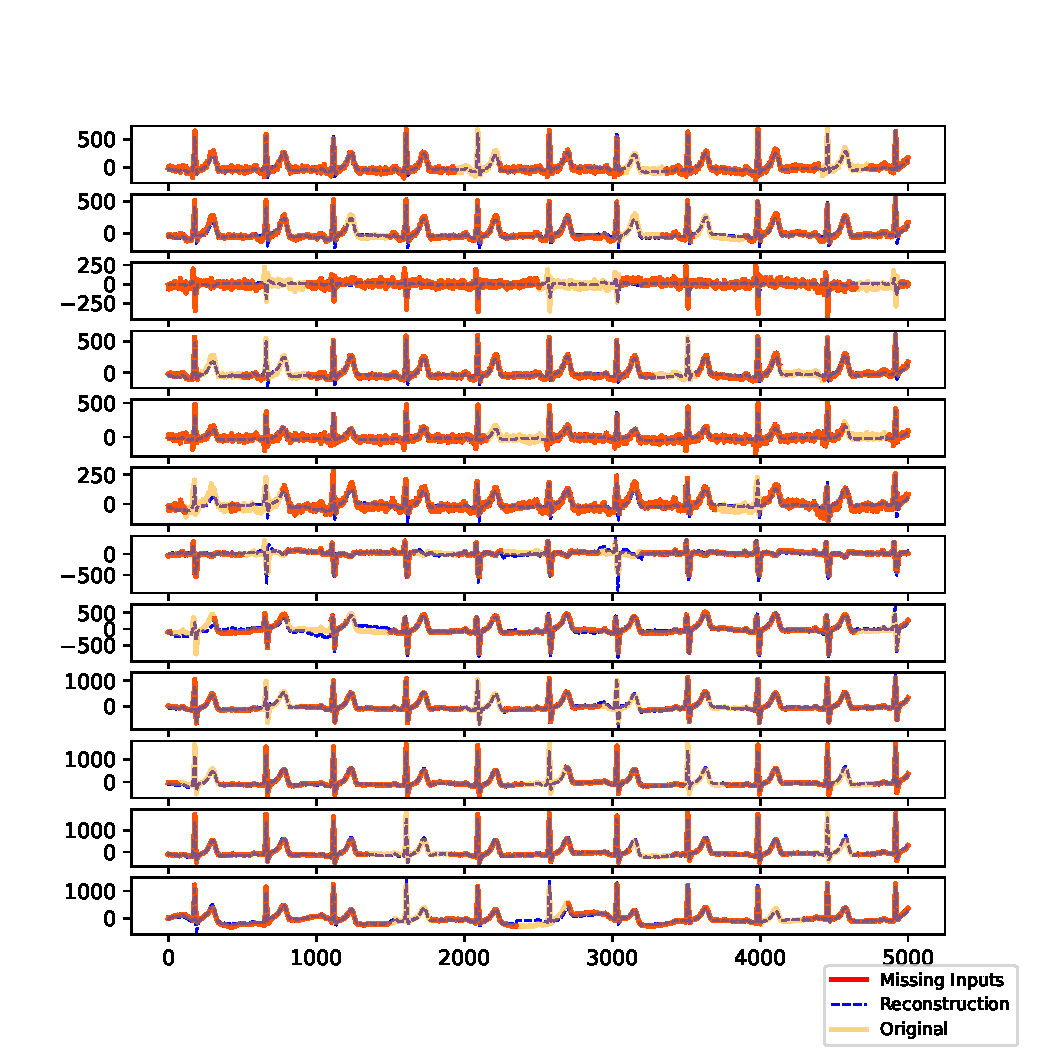
\includegraphics[width=\linewidth]{images/missing/rpsmf_output_20_3.pdf}
    \caption{$20\%$ missing data.}
\end{minipage}%
\hspace{0.05\linewidth}
\begin{minipage}{0.4\linewidth}
    \centering
    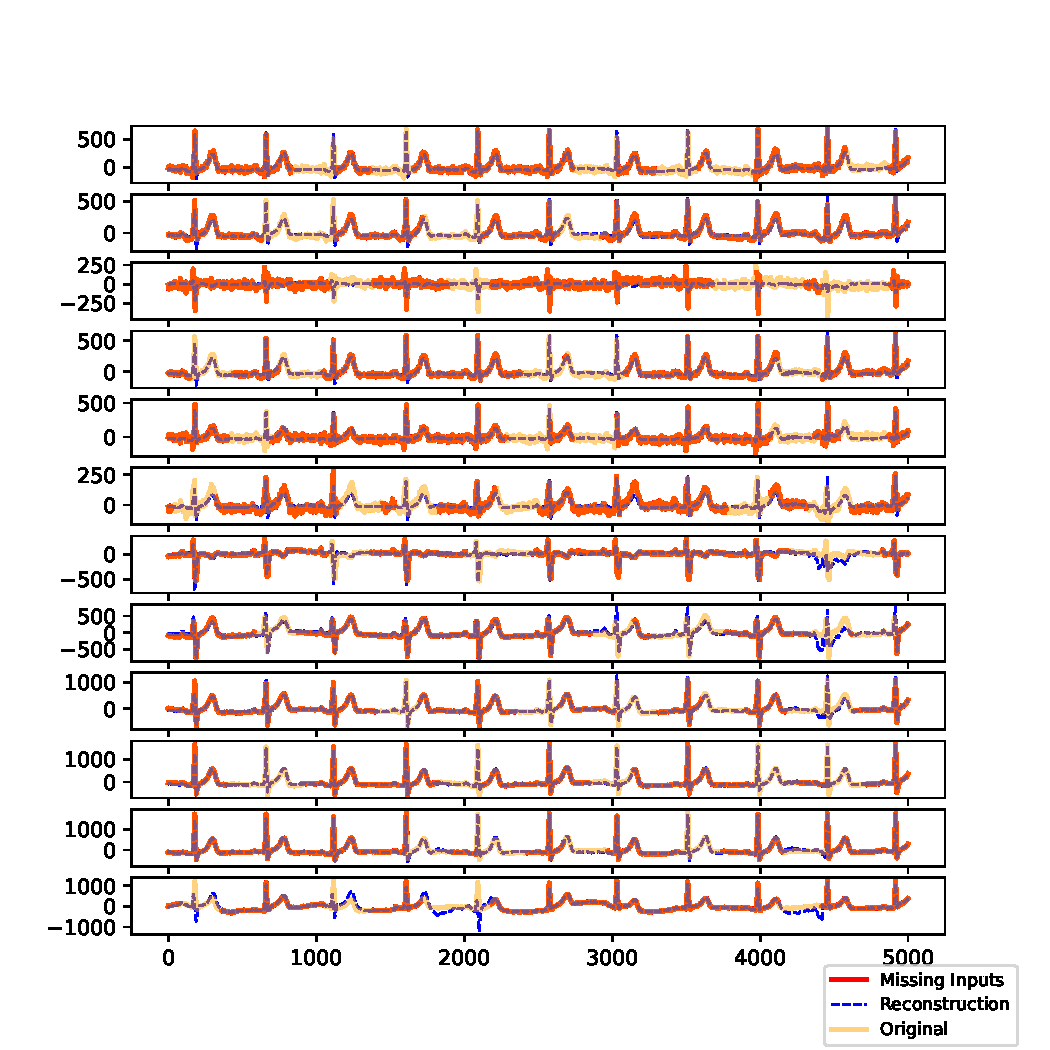
\includegraphics[width=\linewidth]{images/missing/rpsmf_output_30_3.pdf}
    \caption{$30\%$ missing data.}
\end{minipage}

\vspace{1em} % Adjust vertical space between the rows if necessary

% Second row
\begin{minipage}{0.4\linewidth}
    \centering
    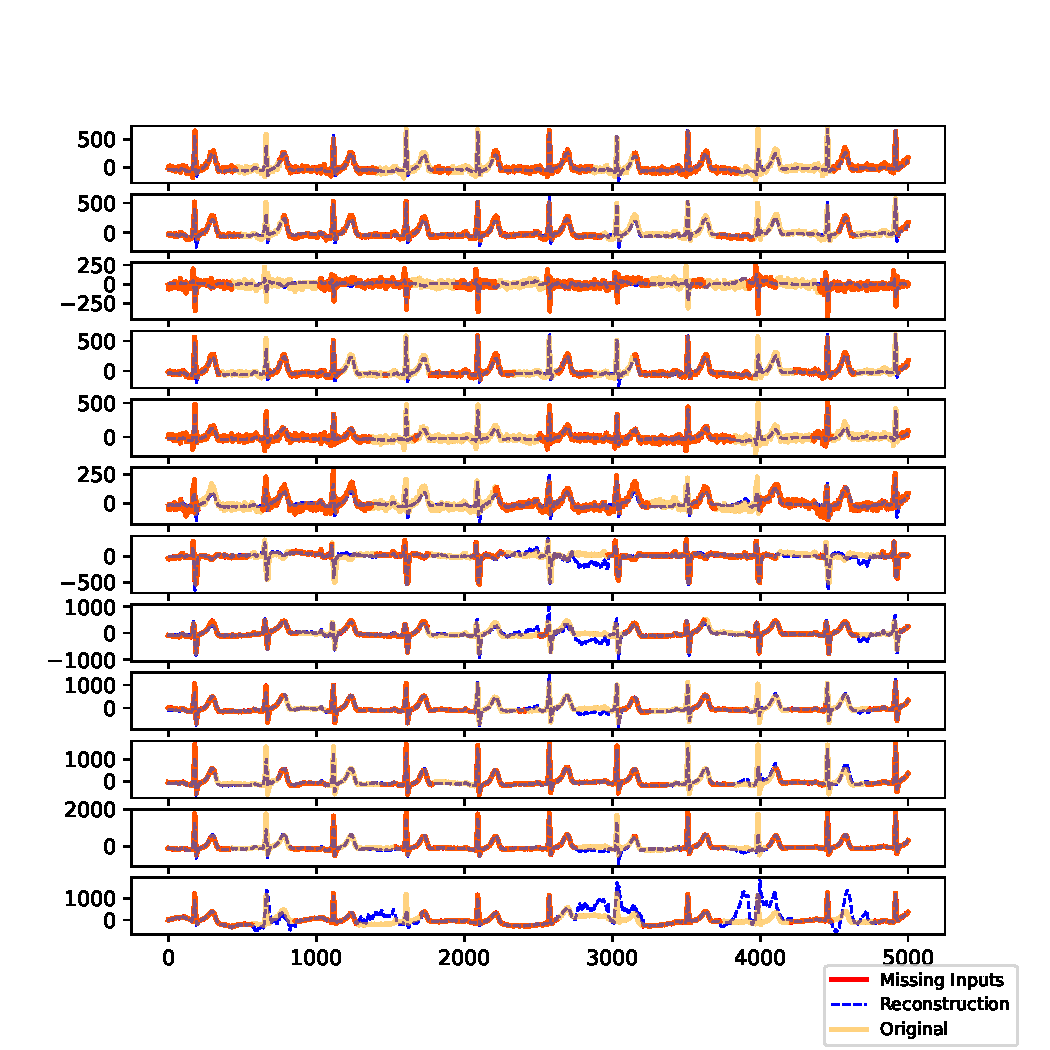
\includegraphics[width=\linewidth]{images/missing/rpsmf_output_40_3.pdf}
    \caption{$40\%$ missing data.}
\end{minipage}
\end{figure}

\subsection{$r = 10$}

\begin{figure}[H]
\centering
% First row
\begin{minipage}{0.4\linewidth}
    \centering
    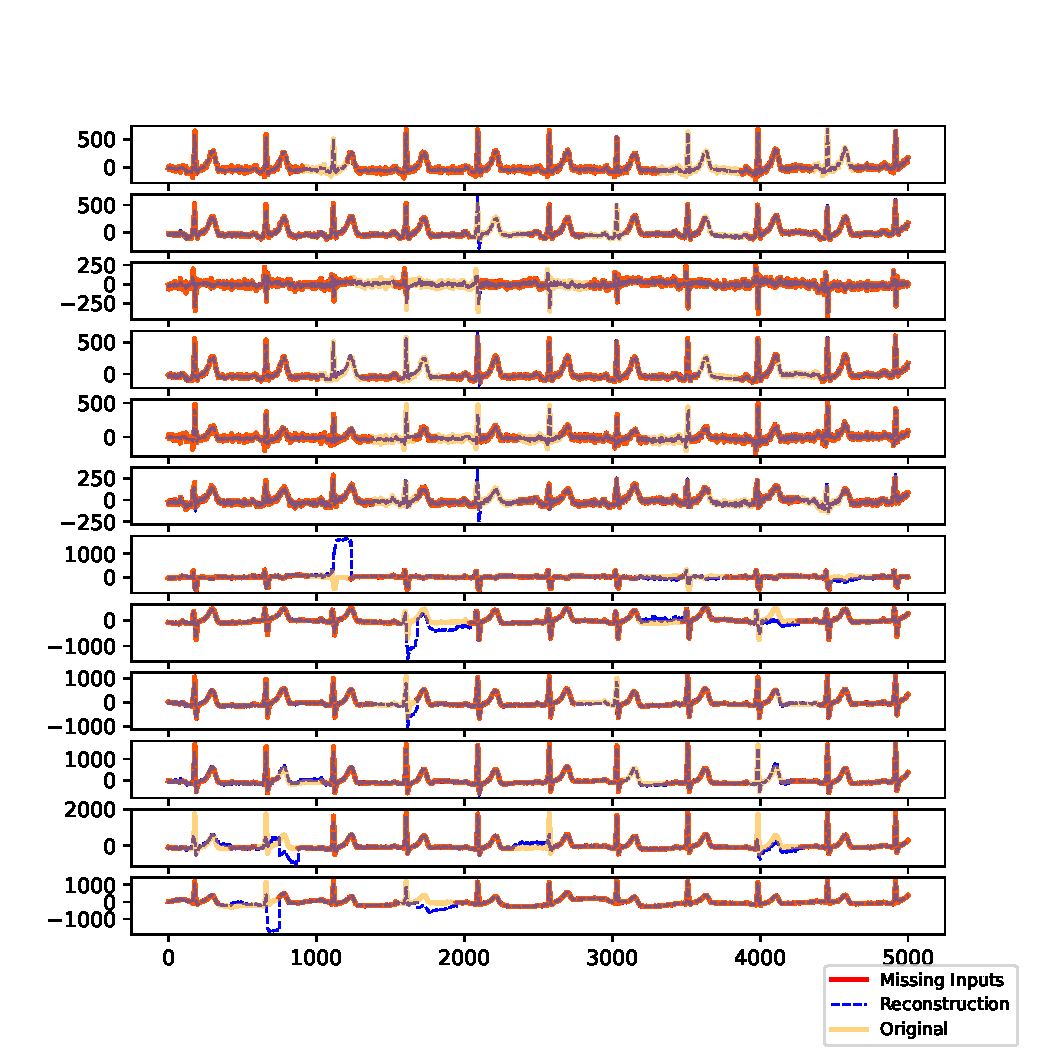
\includegraphics[width=\linewidth]{images/missing/rpsmf_output_20_10.pdf}
    \caption{$20\%$ missing data.}
\end{minipage}%
\hspace{0.05\linewidth}
\begin{minipage}{0.4\linewidth}
    \centering
    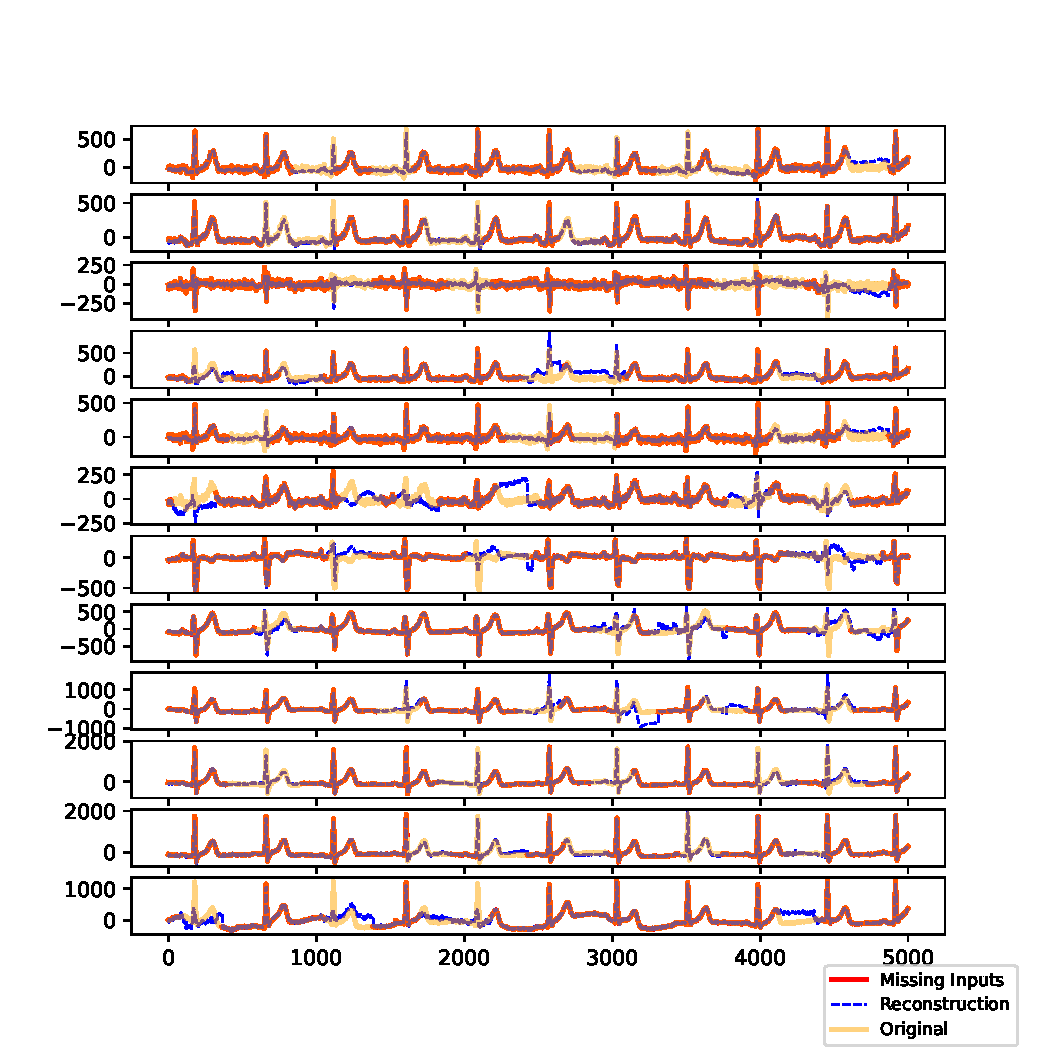
\includegraphics[width=\linewidth]{images/missing/rpsmf_output_30_10.pdf}
    \caption{$30\%$ missing data.}
\end{minipage}

\vspace{1em} % Adjust vertical space between the rows if necessary

% Second row
\begin{minipage}{0.4\linewidth}
    \centering
    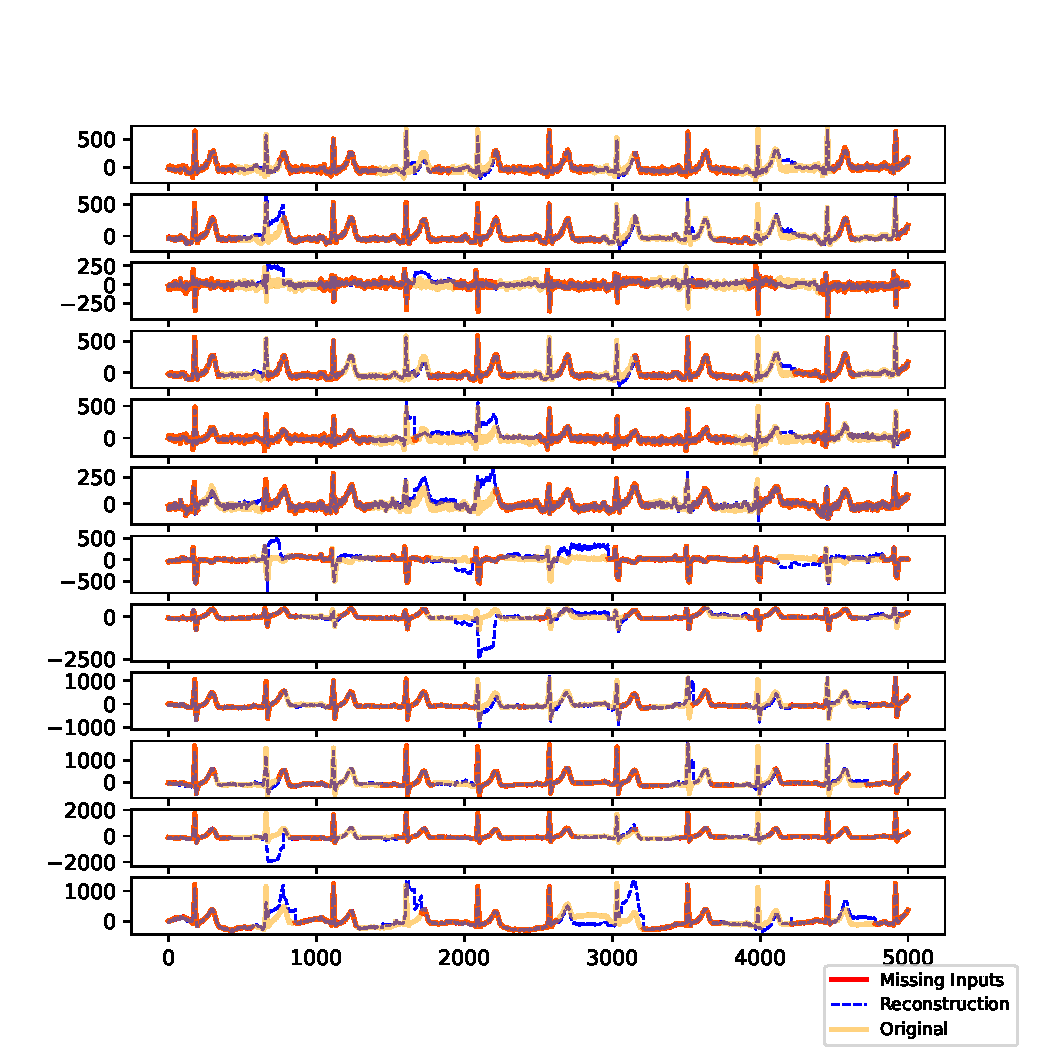
\includegraphics[width=\linewidth]{images/missing/rpsmf_output_40_10.pdf}
    \caption{$40\%$ missing data.}
\end{minipage}
\end{figure}

\section{MLE-SMF}\label{app:mle-smf}

\subsection{$r = 3$}

\begin{figure}[H]
\centering
% First row
\begin{minipage}{0.4\linewidth}
    \centering
    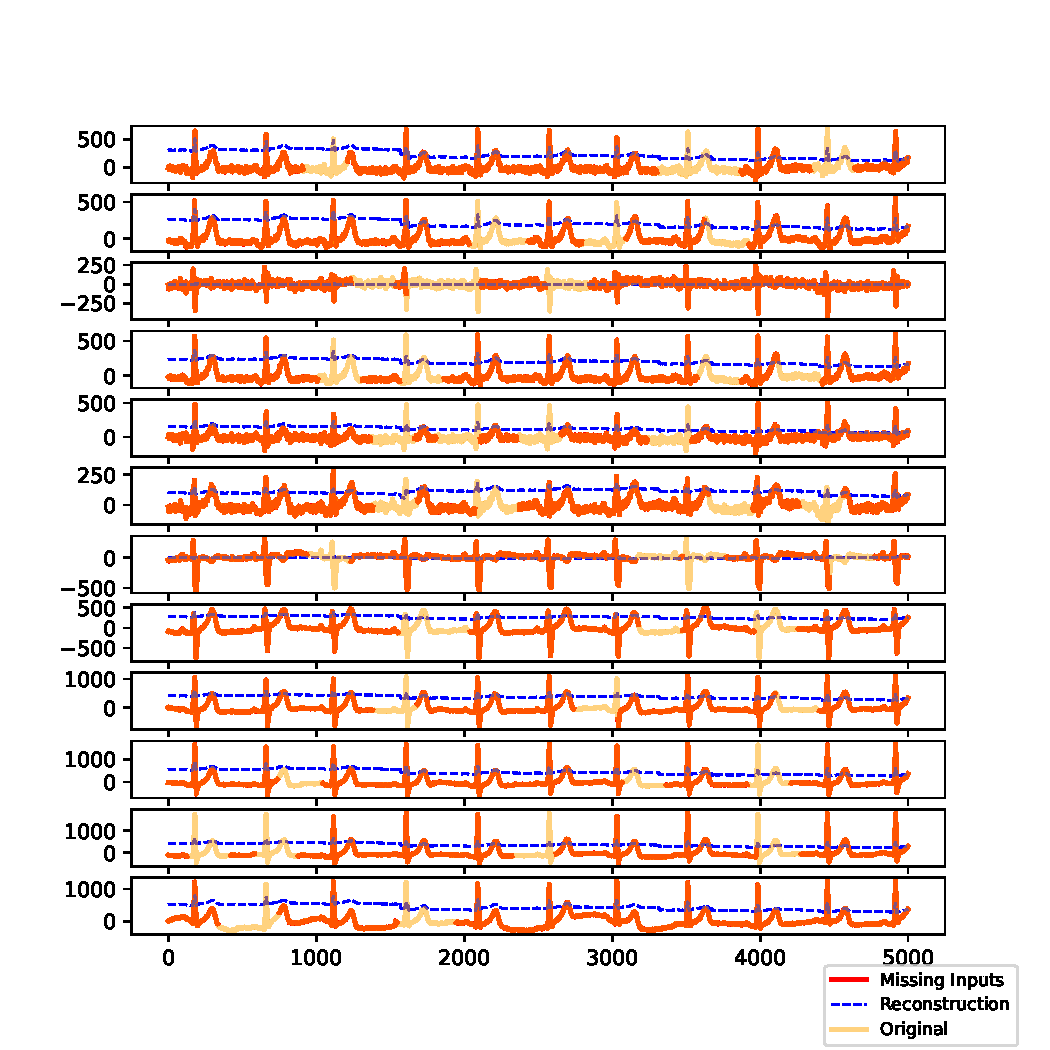
\includegraphics[width=\linewidth]{images/missing/mlesmf_output_20_3.pdf}
    \caption{$20\%$ missing data.}
\end{minipage}%
\hspace{0.05\linewidth}
\begin{minipage}{0.4\linewidth}
    \centering
    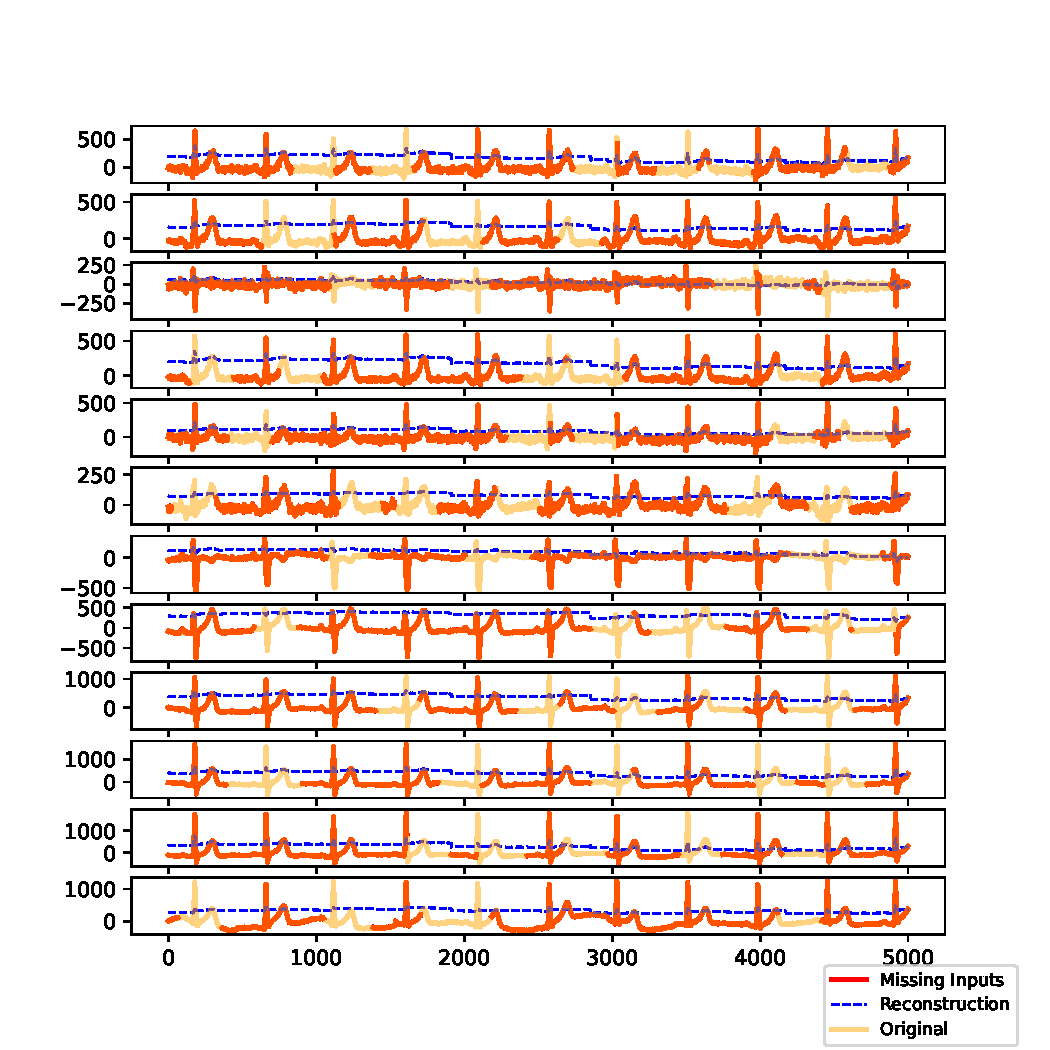
\includegraphics[width=\linewidth]{images/missing/mlesmf_output_30_3.pdf}
    \caption{$30\%$ missing data.}
\end{minipage}

\vspace{1em} % Adjust vertical space between the rows if necessary

% Second row
\begin{minipage}{0.4\linewidth}
    \centering
    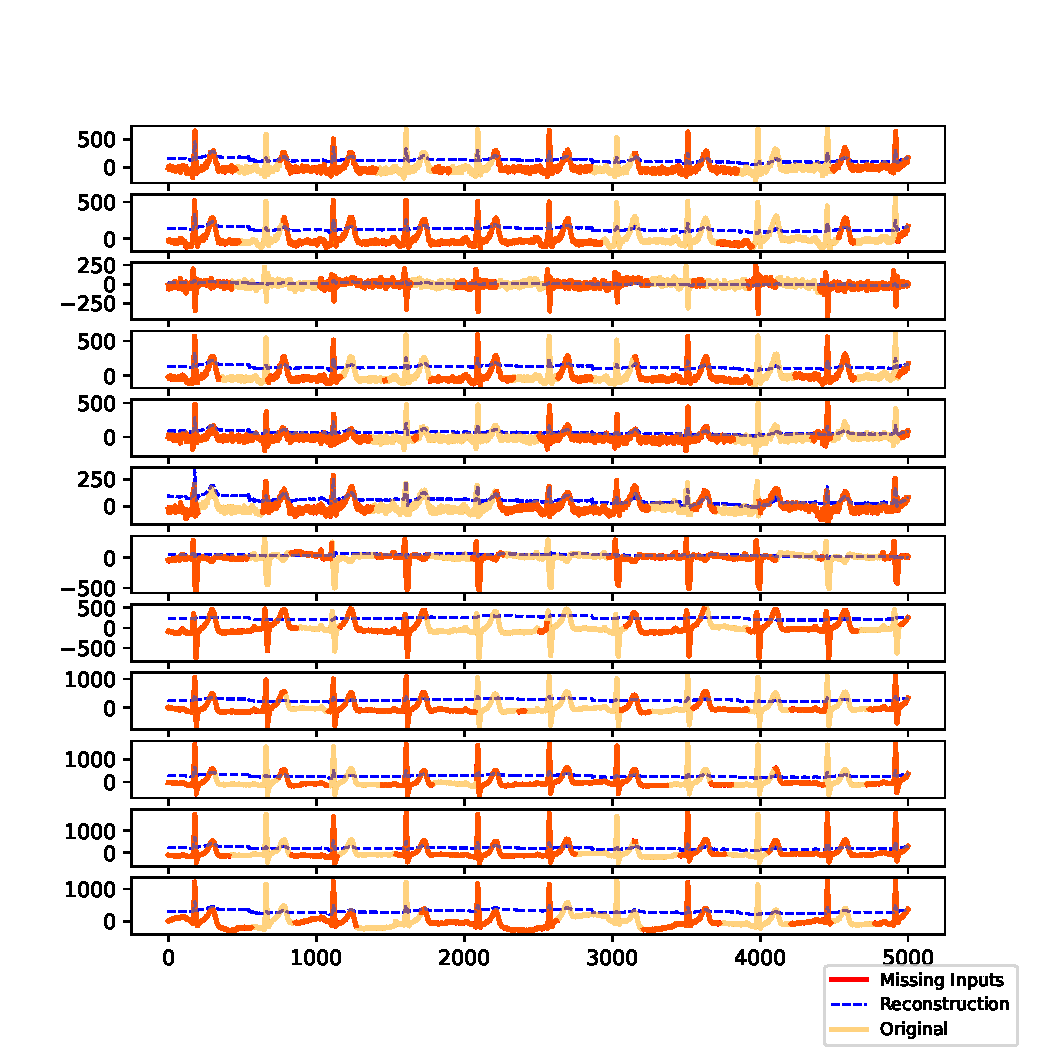
\includegraphics[width=\linewidth]{images/missing/mlesmf_output_40_3.pdf}
    \caption{$40\%$ missing data.}
\end{minipage}
\end{figure}

\subsection{$r = 10$}

\begin{figure}[H]
\centering
% First row
\begin{minipage}{0.4\linewidth}
    \centering
    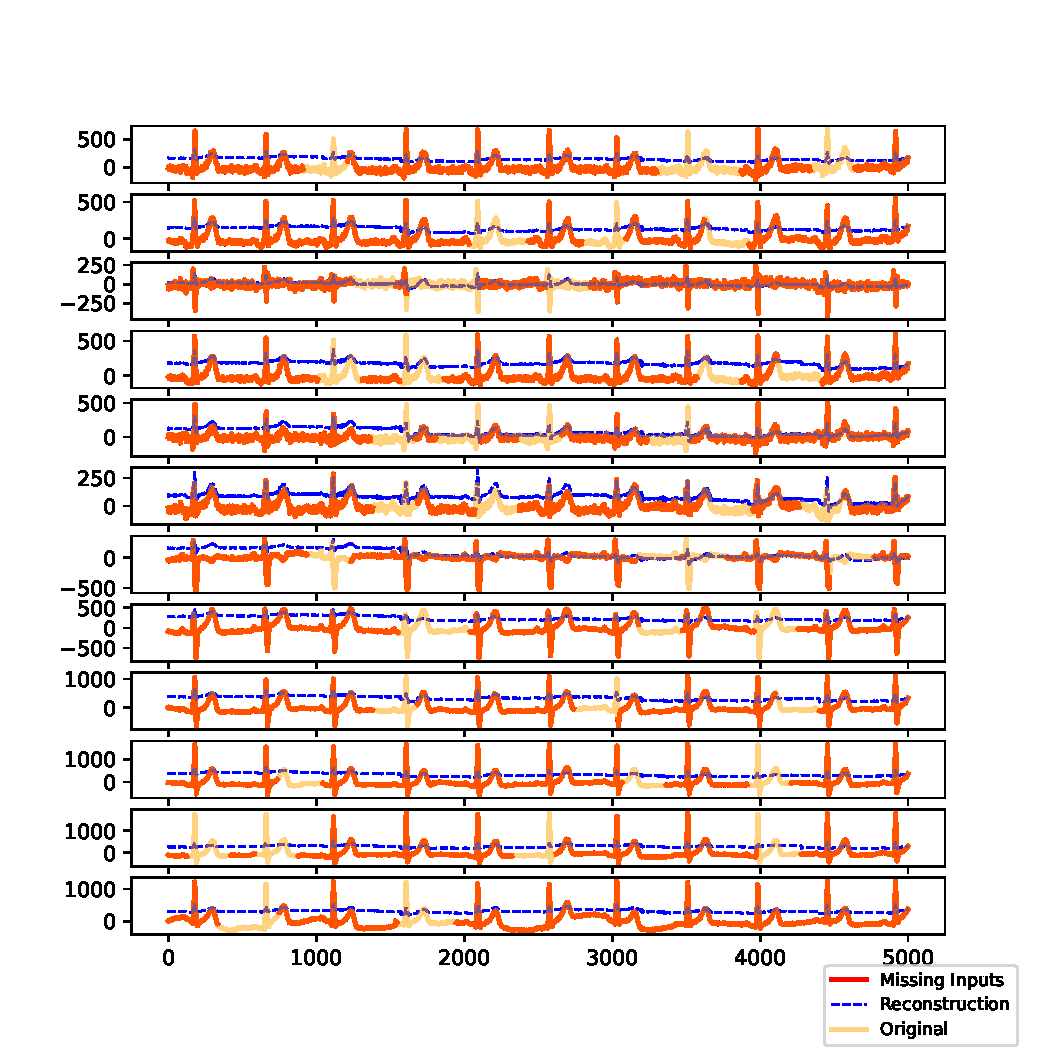
\includegraphics[width=\linewidth]{images/missing/mlesmf_output_20_10.pdf}
    \caption{$20\%$ missing data.}
\end{minipage}%
\hspace{0.05\linewidth}
\begin{minipage}{0.4\linewidth}
    \centering
    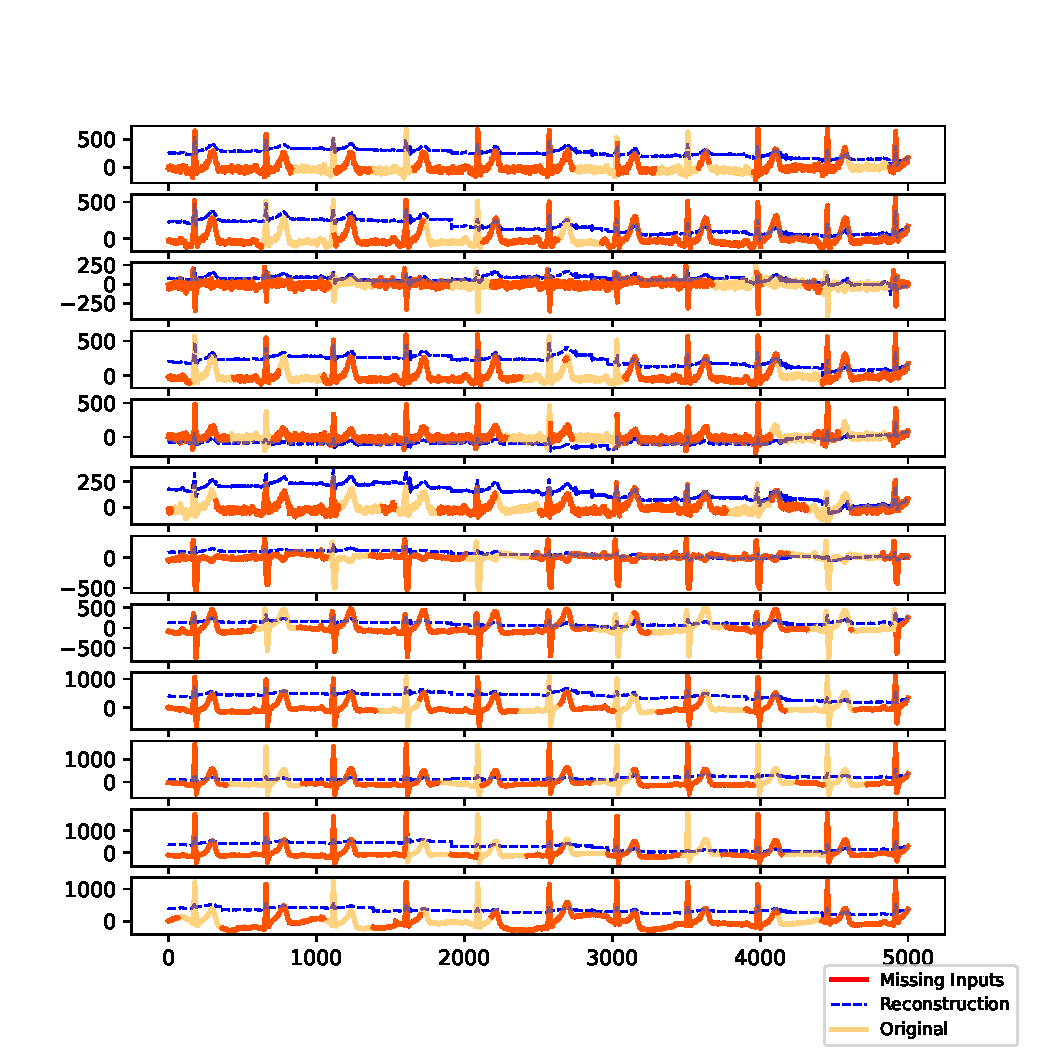
\includegraphics[width=\linewidth]{images/missing/mlesmf_output_30_10.pdf}
    \caption{$30\%$ missing data.}
\end{minipage}

\vspace{1em} % Adjust vertical space between the rows if necessary

% Second row
\begin{minipage}{0.4\linewidth}
    \centering
    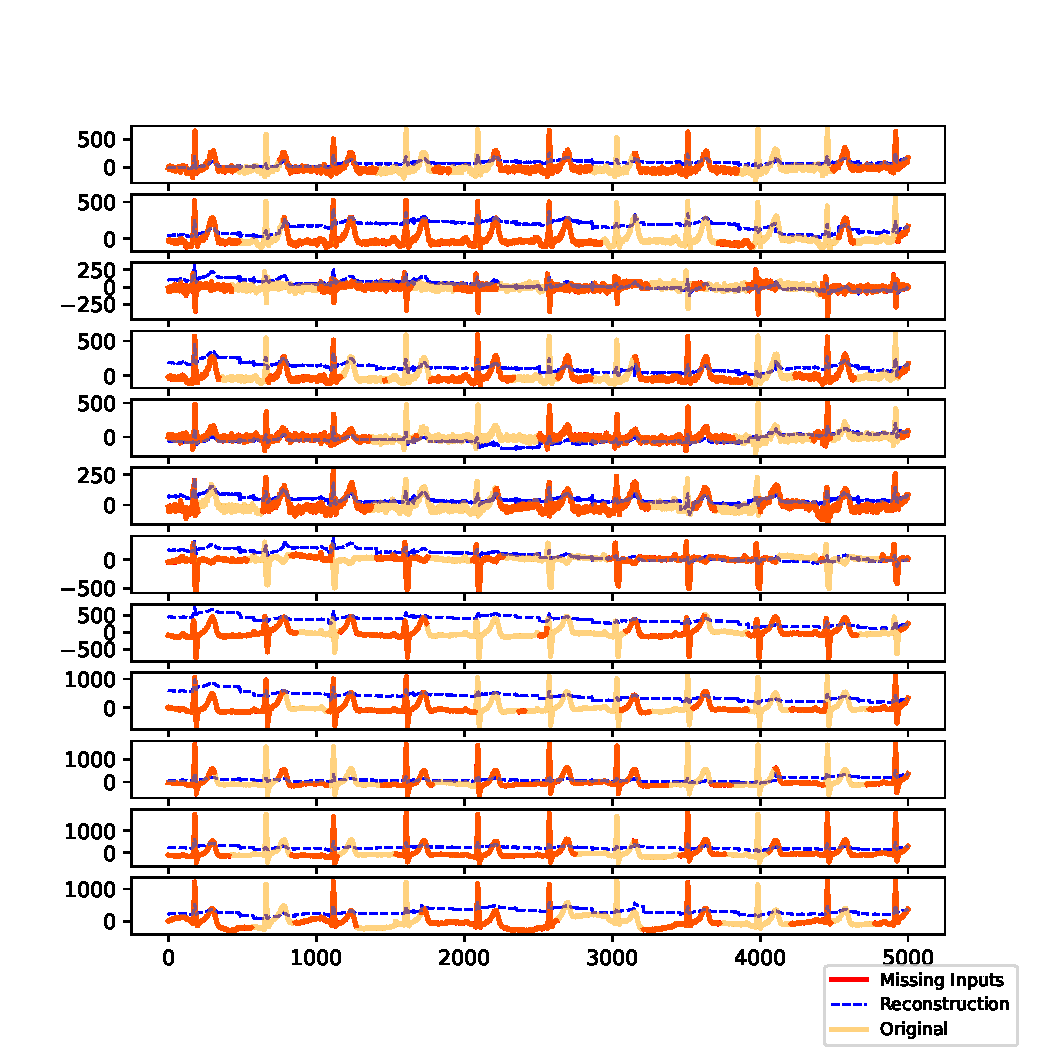
\includegraphics[width=\linewidth]{images/missing/mlesmf_output_40_10.pdf}
    \caption{$40\%$ missing data.}
\end{minipage}
\end{figure}

\section{TMF}\label{app:tmf}

\subsection{$r = 3$}

\begin{figure}[H]
\centering
% First row
\begin{minipage}{0.4\linewidth}
    \centering
    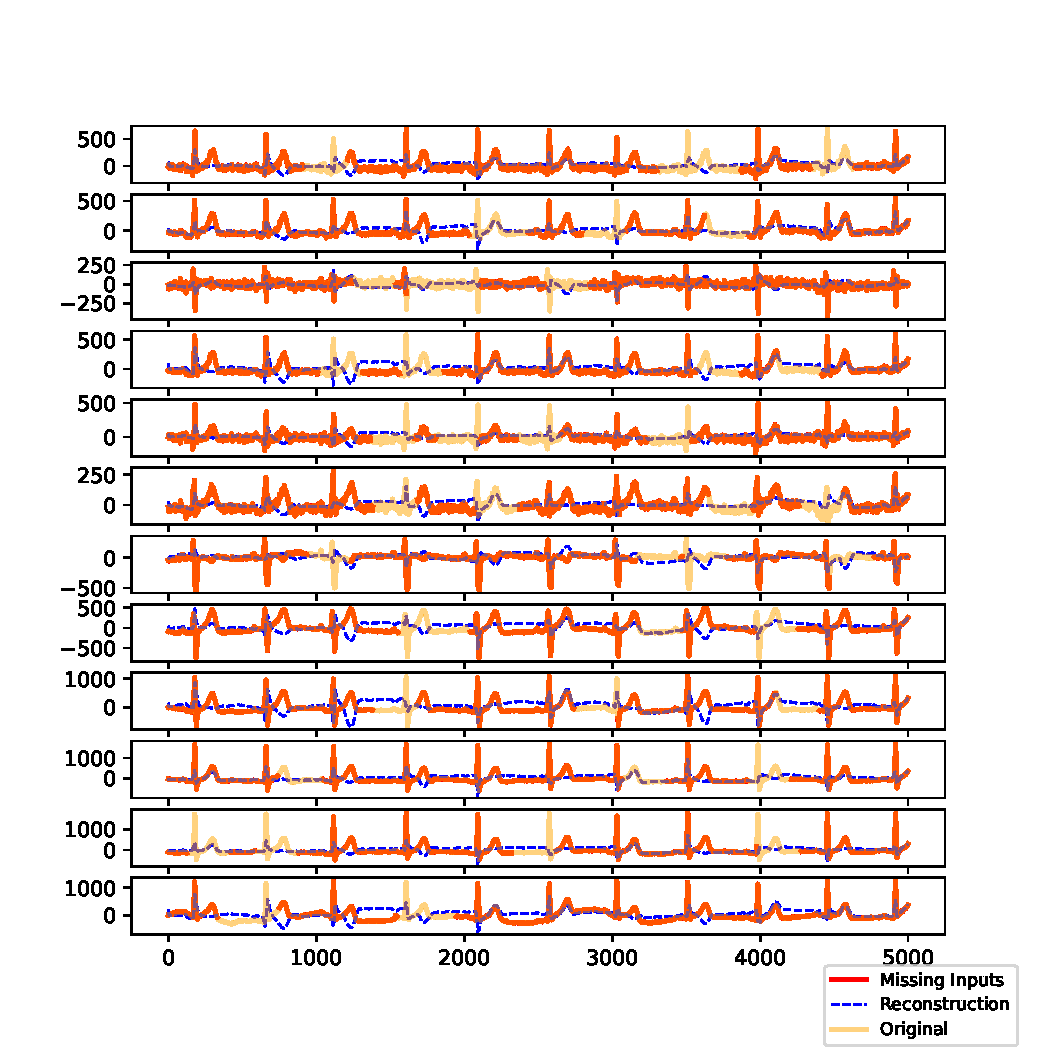
\includegraphics[width=\linewidth]{images/missing/tmf_output_20_3.pdf}
    \caption{$20\%$ missing data.}
\end{minipage}%
\hspace{0.05\linewidth}
\begin{minipage}{0.4\linewidth}
    \centering
    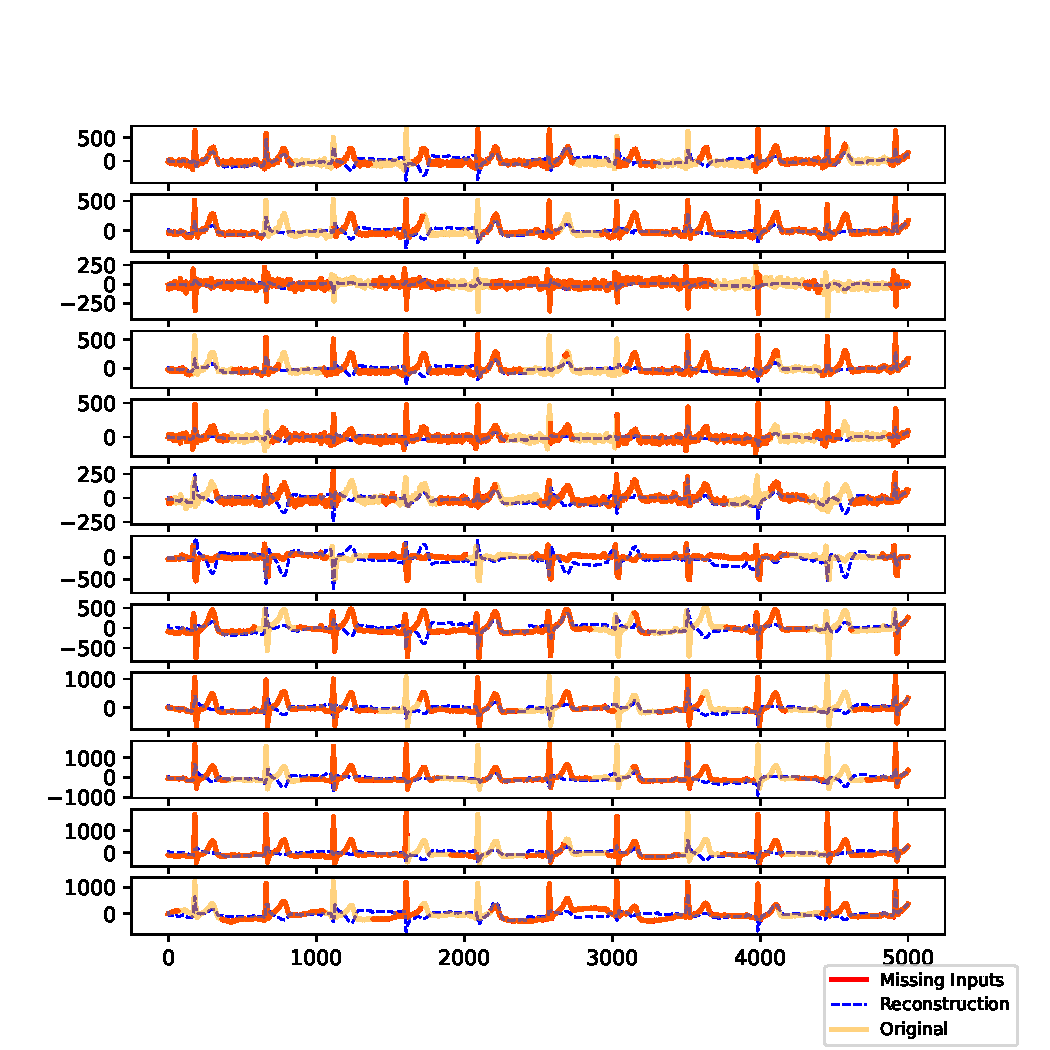
\includegraphics[width=\linewidth]{images/missing/tmf_output_30_3.pdf}
    \caption{$30\%$ missing data.}
\end{minipage}

\vspace{1em} % Adjust vertical space between the rows if necessary

% Second row
\begin{minipage}{0.4\linewidth}
    \centering
    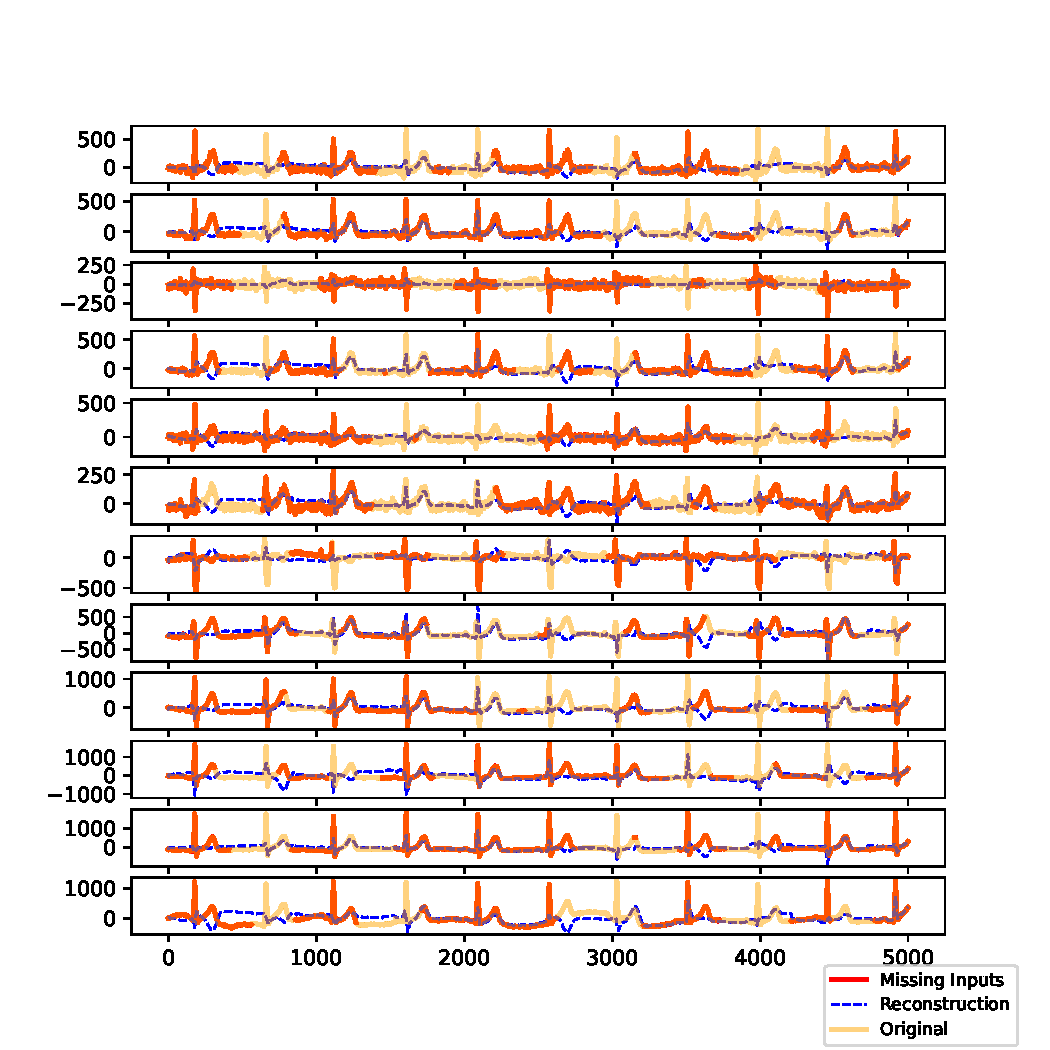
\includegraphics[width=\linewidth]{images/missing/tmf_output_40_3.pdf}
    \caption{$40\%$ missing data.}
\end{minipage}
\end{figure}

\subsection{$r = 10$}

\begin{figure}[H]
\centering
% First row
\begin{minipage}{0.4\linewidth}
    \centering
    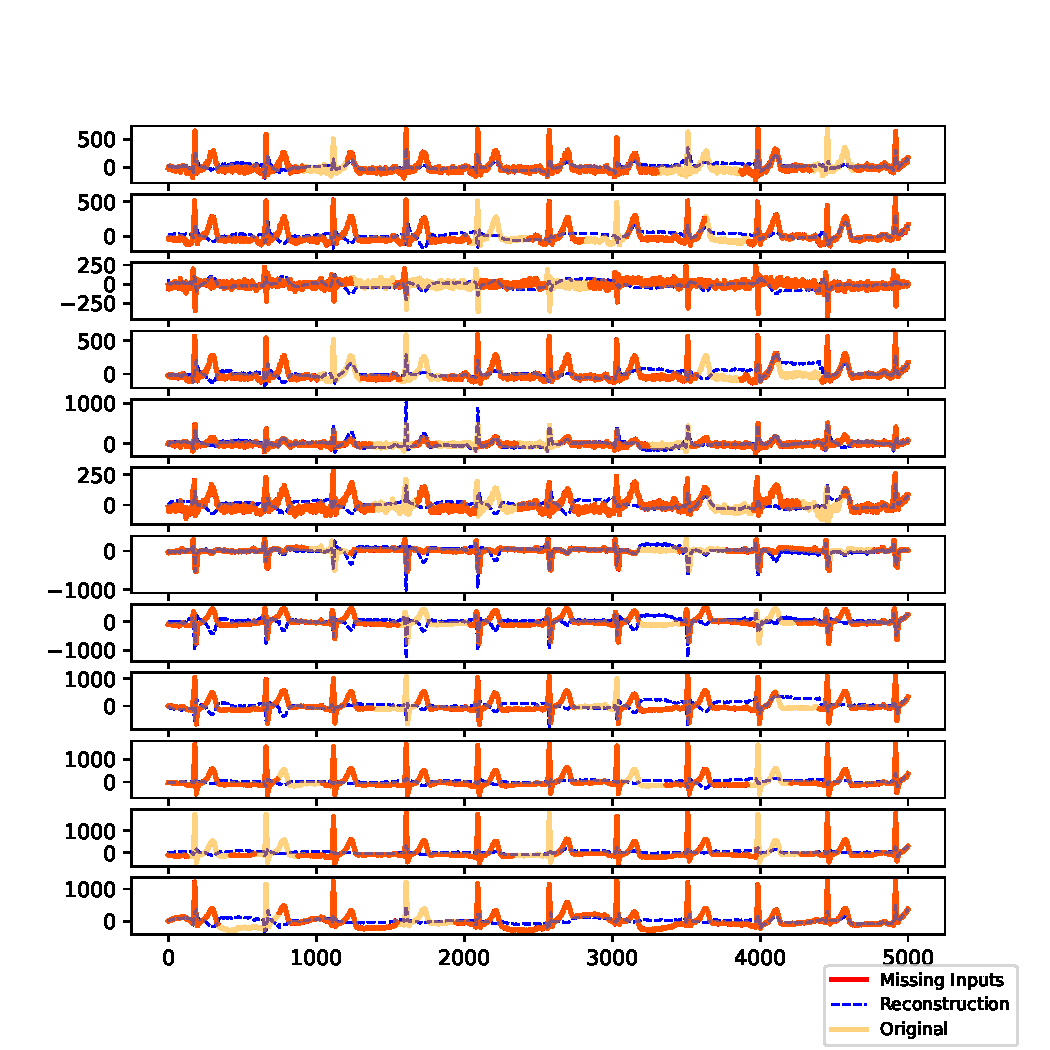
\includegraphics[width=\linewidth]{images/missing/tmf_output_20_10.pdf}
    \caption{$20\%$ missing data.}
\end{minipage}%
\hspace{0.05\linewidth}
\begin{minipage}{0.4\linewidth}
    \centering
    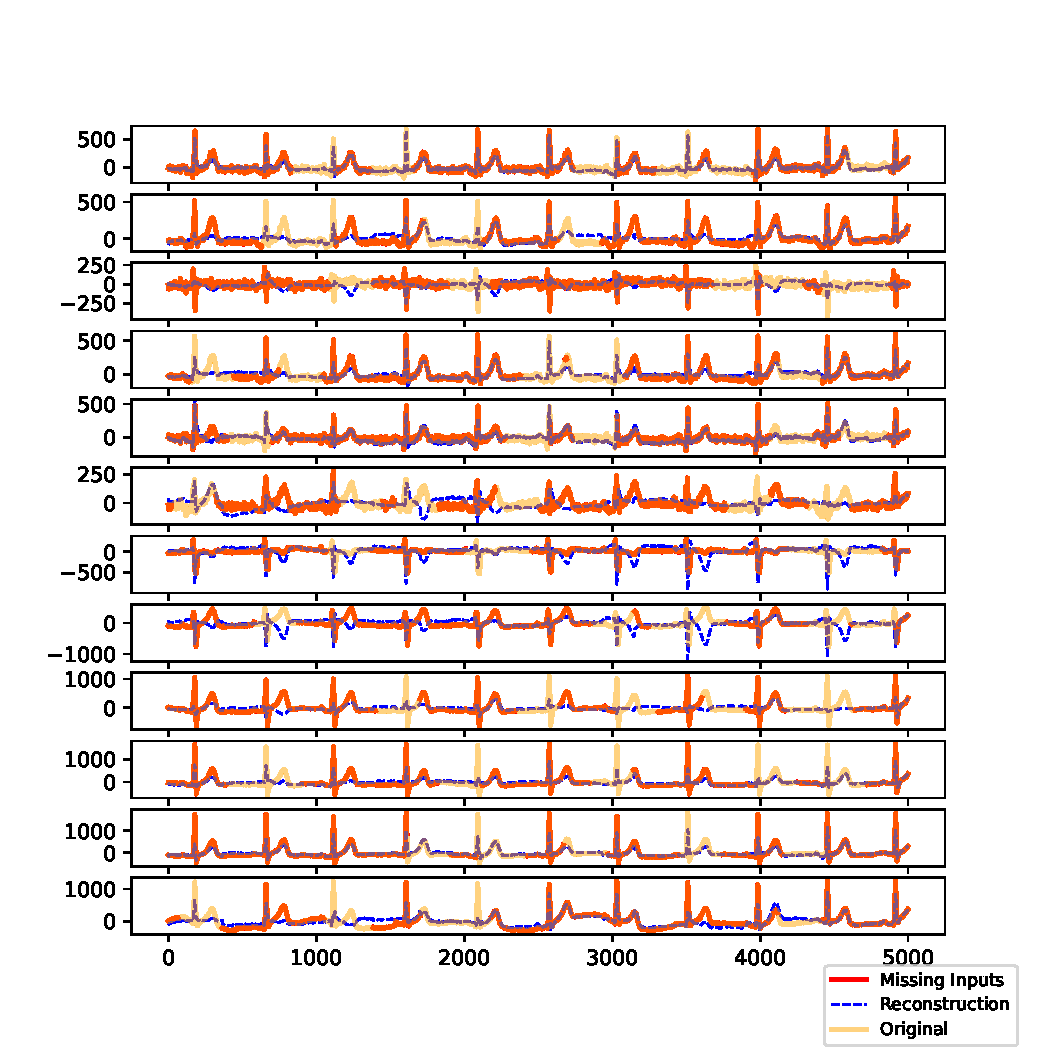
\includegraphics[width=\linewidth]{images/missing/tmf_output_30_10.pdf}
    \caption{$30\%$ missing data.}
\end{minipage}

\vspace{1em} % Adjust vertical space between the rows if necessary

% Second row
\begin{minipage}{0.4\linewidth}
    \centering
    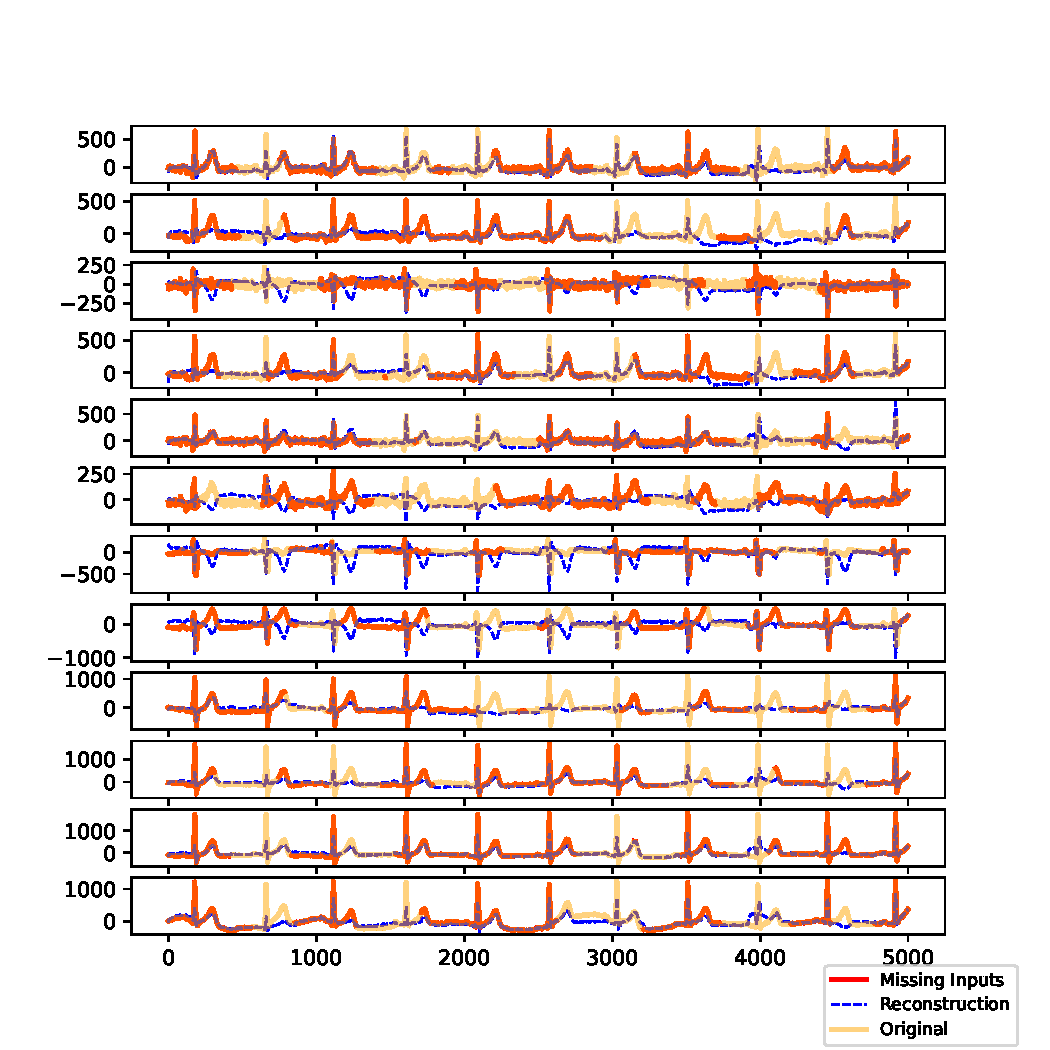
\includegraphics[width=\linewidth]{images/missing/tmf_output_40_10.pdf}
    \caption{$40\%$ missing data.}
\end{minipage}
\end{figure}

\end{document}
